\documentclass[11pt]{article}
\usepackage[T1]{fontenc}
\usepackage[utf8]{inputenc}
\usepackage{lmodern}
\usepackage[letterpaper,margin=1in]{geometry}
\usepackage{amsmath,amssymb,amsthm,mathtools}
\usepackage{microtype}
\usepackage{enumitem}
\usepackage{booktabs,array}
\usepackage{graphicx}
\usepackage{placeins}
\usepackage{tikz}
\usetikzlibrary{arrows.meta,calc,positioning,fit}
\usepackage[numbers,sort&compress]{natbib}
\usepackage{xcolor}
\definecolor{linkblue}{RGB}{28,65,115}
\definecolor{proofblue}{RGB}{44,93,130}
\definecolor{proofgray}{RGB}{245,247,249}
\usepackage{xurl}
\usepackage[colorlinks=true,linkcolor=linkblue,citecolor=linkblue,
  urlcolor=linkblue,bookmarksnumbered=true,bookmarksdepth=2]{hyperref}
\newcommand{\doi}[1]{\begingroup\urlstyle{rm}doi:
  \href{https://doi.org/#1}{\nolinkurl{#1}}\endgroup}
\hypersetup{pdftitle={Failure of finite assembly for a chromatic overlap at the prime three},
 pdfauthor={OpenAI},pdfkeywords={Failure-of-finite-assembly-for-a-chromatic-overlap-at-the-prime-three-September-25-2026},pdfsubject={Chromatic overlaps, continuous cohomology, and ordinary thick subcategories}}
\IfFileExists{glyphtounicode.tex}{\input{glyphtounicode}}{}
\IfFileExists{glyphtounicode-cmex.tex}{\input{glyphtounicode-cmex}}{}
\ifdefined\pdfgentounicode\pdfgentounicode=1\fi
\ifdefined\pdfinfoomitdate\pdfinfoomitdate=1\fi
\ifdefined\pdftrailerid\pdftrailerid{}\fi
\ifdefined\pdfsuppressptexinfo\pdfsuppressptexinfo=15\fi

\newtheorem{theorem}{Theorem}[section]
\newtheorem{lemma}[theorem]{Lemma}
\newtheorem{proposition}[theorem]{Proposition}
\newtheorem{corollary}[theorem]{Corollary}
\theoremstyle{definition}
\newtheorem{definition}[theorem]{Definition}
\newtheorem{conjecture}[theorem]{Conjecture}
\newtheorem{remark}[theorem]{Remark}
\newtheorem{example}[theorem]{Example}
\numberwithin{equation}{section}
\newcommand{\Qp}{\mathbb Q_p}
\newcommand{\Zp}{\mathbb Z_p}
\newcommand{\Fp}{\mathbb F_p}
\DeclareMathOperator{\Nrd}{Nrd}
\DeclareMathOperator{\Spa}{Spa}
\DeclareMathOperator{\Spf}{Spf}
\DeclareMathOperator{\Hom}{Hom}
\DeclareMathOperator{\End}{End}
\DeclareMathOperator{\Aut}{Aut}
\DeclareMathOperator{\Lie}{Lie}
\DeclareMathOperator{\Spec}{Spec}
\DeclareMathOperator{\Thick}{Thick}
\DeclareMathOperator*{\colim}{colim}
\DeclareMathOperator{\coker}{coker}
\DeclareMathOperator{\im}{im}
\DeclareMathOperator{\id}{id}
\DeclareMathOperator{\Tot}{Tot}
\DeclareMathOperator{\Perf}{Perf}
\newcommand{\Ccts}{C^\bullet_{\mathrm{cts}}}


\setlist[enumerate]{label=\textup{(\roman*)},leftmargin=*,itemsep=3pt}
\setlist[itemize]{leftmargin=*,itemsep=3pt}
\setlength{\emergencystretch}{2em}
\title{Failure of finite assembly for a chromatic overlap\\
at the prime three}
\author{OpenAI}
\date{September 25, 2026}

\begin{document}
\maketitle
\begin{abstract}
At the prime three and height three, the chromatic overlap cannot be
constructed from the rational, height-one, and height-two local spheres by
finitely many sums, shifts, cofibers, and retracts in the category of
\(E(2)\)-local modules over the derived 3-complete sphere. This gives a
negative answer to the ordinary finite-assembly question for chromatic
overlaps.
\end{abstract}

\begingroup
\setcounter{tocdepth}{1}
\small\tableofcontents
\endgroup

\section{Introduction}\label{sec:introduction}

Chromatic fracture reconstructs a spectrum from its local pieces and the
maps relating adjacent heights. For the sphere, one of the objects that
carries this gluing information is the overlap
\[
                         L_{n-1}L_{K(n)}S.
\]
Here \(S=S_p^\wedge\) is the derived \(p\)-complete sphere,
\(L_i\) denotes localization with respect to Johnson--Wilson theory
\(E(i)\), \(L_0\) is rationalization, and \(L_{K(n)}\) denotes Morava
\(K(n)\)-localization. Classical chromatic splitting asks for a precise
description of this overlap by lower local spheres
\citep{Hovey93,BB19}. We study the less restrictive question of whether
those spheres can produce the overlap by any finite construction.

For objects \(X_1,\ldots,X_r\) in the category of \(E(n-1)\)-local
\(S\)-modules, let
\(\Thick\{X_1,\ldots,X_r\}\) be the smallest full subcategory containing
them and closed under equivalences, finite sums, integer suspensions and
desuspensions, homotopy cofibers, and retracts
\citep[Definitions~1.2, 1.3(c), and 1.5(c)]{HS99}. Every map is \(S\)-linear.
This is the \emph{ordinary} thick subcategory: tensoring with an arbitrary
module, taking an infinite coproduct, or taking an unrestricted homotopy
limit is not an additional closure operation. The finite-assembly question
asks whether
\begin{equation}\label{eq:finite-assembly-question}
 L_{n-1}L_{K(n)}S\in
       \Thick\{L_0S,L_1S,\ldots,L_{n-1}S\}
\end{equation}
for every prime \(p\) and every \(n\geq1\). The number of cofibers and their
attaching maps may depend on \(p\) and \(n\). In particular, this question
allows nonsplit extensions and Moore corrections: a cofiber of multiplication
by a power of \(p\) is one of the permitted constructions.

\begin{theorem}\label{thm:main}
At \(p=n=3\), with \(S=S_3^\wedge\),
\[
             L_2L_{K(3)}S
                  \notin\Thick\{L_0S,L_1S,L_2S\}
\]
in the category of \(E(2)\)-local \(S\)-modules.
\end{theorem}

This disproves the ordinary finite-assembly statement
\eqref{eq:finite-assembly-question}. Its scope is the specified prime and
height. The obstruction does not depend on a proposed list of summands or
on a bound for the number of allowed cofibers.

\subsection{Splittings, finite constructions, and the prime three}

The historical splitting assertions contain more data than ordinary thick
membership. In Hovey's account of Hopkins' conjecture, the proposed exterior
classes, factorizations, and summands are distinguished from the splitting
of the canonical cofiber sequence
\citep[Conjecture~4.2]{Hovey93}. The detection result there is conditional
on chromatic splitting \citep[Theorem~4.3]{Hovey93}. For the sphere, the
weak splitting question asks only whether the canonical unit
\[
          L_{n-1}S\longrightarrow L_{n-1}L_{K(n)}S
\]
has a retraction; the finite-input formulation is stated in
\citet[Conjecture~1.1.11]{BGH2022}. Ordinary thick membership records no
distinguished map at all. A prescribed strong decomposition with its unit
would give both a finite construction and a weak splitting, but a finite
construction may have nonsplit attachments and need not split that unit.

At height two, the positive odd-prime results developed from
Shimomura--Yabe's calculation for \(p\geq5\)
\citep[Theorem~2.4]{ShimomuraYabe95}, revisited and corrected by
\citet[Theorem~7.7 and Remark~7.8]{Behrens12}.
At the prime three, Goerss--Henn--Mahowald established the prescribed
height-two splitting \citep[Theorem~5.11]{GHM14}.
Thus prime three admits a height-two splitting, while
Theorem~\ref{thm:main} obstructs even finite assembly at the next height.
The prime-two case explains why failure of a prescribed list need
not obstruct finite assembly. Beaudry disproved the original strong
wedge formula at \(n=p=2\)
\citep[Theorem~1.4]{Beaudry2017}. Beaudry--Goerss--Henn then described the
additional Moore-spectrum terms while retaining the canonical unit
retraction \citep[Theorem~1.1.6]{BGH2022}. Those extra terms are allowed by
the ordinary thick closure above. Thus the known failure of a prescribed
wedge is not by itself an obstruction to finite assembly. Conversely,
Theorem~\ref{thm:main} addresses the finite-construction question, not the
separate assertion that a particular canonical unit fails to retract.
The revised strong summand patterns and their known low-height cases are
discussed in \citet[Section~6.1]{BB19}.

The companion article \emph{Filtered chromatic splitting at generic primes}
constructs an actual filtration by lower local spheres for \(n\geq1\) and
\(p>n+1\) \citep[Theorem~1.1]{CompanionFiltered}. Its prime range excludes
the example studied here. The companion rational obstruction at height three
concerns a prescribed strong wedge for \(p\geq5\)
\citep[Corollary~1.2]{CompanionRational}; such an obstruction is compatible
with a finite construction by nonsplit cofibers. Neither companion result
supplies a step in the prime-three proof below.

The connected-marking method has earlier coheight-one precedents.
Torii's Laurent-field coefficient tower builds on Gross's monodromy
calculation and carries commuting stabilizer actions from the two heights
\citep[Theorem~3.5(1a)]{Gross79}
\citep[Theorems~2.7 and 2.9 and Corollary~2.8]{Torii03}.
Torii later constructed a localized Adams spectral sequence and detected
the degree-minus-one reduced-norm class in actual iterated localization
\citep[Theorems~4.7 and 8.1]{Torii11}. The present obstruction requires
further comparisons that retain the exceptional norm character through
ordinary finite-stage coefficients and the full lower-height deformation.

The geometric starting point is the coheight-one work of
\citet{BMR26}. For odd \(p\) and \(h\geq2\), their theorem has an
exceptional branch when \(p-1\) divides \(h-1\)
\citep[Theorem~A]{BMR26}. The calculation of the completed orientation line
assumes \(k\supseteq\mathbb F_{p^{h(h-1)}}\). At \(p=h=3\), with our choice
\(k\supseteq\mathbb F_{3^6}\), the tame determinant invariants retain a second
cohomology line with a nontrivial lower-height
norm character \citep[Theorem~D, Theorems~3.6.10 and~5.2.10, and Lemma~5.2.5]{BMR26}.
Their completed proxy does not by itself identify the
ordinary overlap used here; in particular, an invertible cofiber for the
proxy does not decide whether its attachment splits
\citep[Theorem~A and Remark~5.2.12]{BMR26}.
The shifted orientation line has a representation-theoretic antecedent in
Heyer's derived Steinberg coinvariant calculation
\citep[Corollary~5.3.4]{Heyer23}
\citep[Lemma~4.1.6 and Corollary~4.3.10]{HeyerGeo24}, used geometrically in
\citet[Sections~3.5--3.6]{BMR26}. Section~\ref{sec:analytic} computes the
required distribution orientation with the coefficient topology used here.
The proof below must carry the character from finite marking coefficients
to ordinary homotopy and retain the whole height-two deformation along the
way. These are the two places where a closed-fiber geometric calculation
alone is insufficient.

\subsection{A detector that is stable under finite construction}

The final obstruction can be stated before its coefficient calculation.
Choose a finite field \(k\) containing \(\mathbb F_{3^6}\), enlarged by a
finite extension when needed to fix the constant identifications, and let
\(E_2=E_2(k)\) be height-two Morava \(E\)-theory. Its degree-zero ring is
\(W(k)[[x]]\); the variable \(x\) is the height-two deformation parameter.
Write \(\omega=\pi_2E_2\) for the periodicity line and
\[
       Q_x=k((x)),\qquad
       \overline\omega=(\omega/3)\otimes_{k[[x]]}Q_x.
\]
An unramified quadratic field \(F/\mathbb Q_3\) lies in the height-two
endomorphism algebra. Its unit group \(G_F=\mathcal O_F^\times\) acts on
\(Q_x\) and on \(\overline\omega\). The action is semilinear: it acts on
scalars as well as on vectors.

For a spectrum \(X\), apply the exact test
\[
 \mathcal T(X)=L_{K(2)}(E_2\wedge X)/3,
 \qquad
 \mathcal V_d(X)=\pi_d\mathcal T(X)\otimes_{k[[x]]}Q_x.
\]
The smash product here is the ordinary smash product of spectra.
After \(K(2)\)-localization the three proposed generators become
\(0,0,L_{K(2)}S\), and the test of the last one has one periodicity line
in each even degree. Exactness now gives a stringent necessary condition:
if \(X\) comes from the local unit by the permitted finite operations, then
every \(\mathcal V_d(X)\) is finite-dimensional and every simple
constituent is a power of \(\overline\omega\).
Proposition~\ref{prop:constituent-test} proves this by placing those
representations in a Serre subcategory. Finite dimensionality is a
consequence on the thick closure, not an assumption about the overlap.

The coefficient calculation produces a different line,
\begin{equation}\label{eq:intro-norm-line}
 Q_x(\delta),\qquad
 \delta(g)=\overline{N_{F/\mathbb Q_3}(g)}
       \in\mathbb F_3^\times,\quad g\in G_F.
\end{equation}
The notation means that \(Q_x\) has its usual semilinear action and a chosen
basis is multiplied by the constant \(\delta(g)\). The character is
nontrivial, since the residue norm
\(\mathbb F_9^\times\to\mathbb F_3^\times\) is surjective. What matters is
not merely this residue character but its action over the field \(Q_x\).
The full group \(G_F\), including its principal units, has infinite image
on \(Q_x\) and fixed field \(k\). Together with the first Hasse invariant,
this full action excludes the norm line from every periodicity power;
Lemma~\ref{lem:generic-character} gives the argument.

\subsection{From finite markings to actual homotopy}

The coefficient calculation and its passage to homotopy solve different
problems. The first produces the norm line in ordinary continuous
cohomology. The second retains that line through the entire height-two
deformation and the filtration of actual homotopy. We describe the
interfaces between these arguments before constructing their coefficients.

\paragraph{Integral markings.}
On the height-two stratum of the height-three deformation, the algebraic
\(p\)-divisible group has a connected part of height two and an
\'etale quotient of height one. Its finite torsion kernels are formed
before passing to the stratum, so both parts are retained. Over the
one-parameter field \(K=k((t))\), let \(L^U\) be the finite \'etale
algebra of connected markings modulo an open subgroup \(U\) of the
height-two stabilizer \(J\). Put
\[
 L=\colim_{U\subset J}L^U,\qquad R=L^{\mathrm{perf}}.
\]
The groups \(P\) and \(J\) are the unextended height-three and height-two
stabilizers, respectively; both fix \(k\). The group \(P\) transports the
deformation, commuting with the marking action of \(J\). Section~\ref{sec:towers}
constructs a determinant-normalized integral marking of the \'etale
quotient. The normalization determines the norm action on the coefficients.
Relative section-sheaf full faithfulness
\citep[Corollary~3.11]{ALB25} makes this a construction of families of
markings, including their frame changes.

\paragraph{Ordinary cohomology.}
The geometry first computes cohomology with the completed perfection of
each finite stage \(L^U\). Returning to ordinary coefficients is a
separate argument: a cochain with values in \(L\) or \(R\) must have its
image in one complete finite marking or root stage. The central step in
Section~\ref{sec:decompletion} proves finite cohomology at such stages.
It uses an invariant differential to normalize Cartier's operator, whose
residue adjoint is Frobenius
\citep[Chapter~II, Section~6]{Cartier58}
\citep[Proposition~9]{Serre58Topology}. This finiteness controls primitives
of small cocycles and allows passage from root stages to completed
perfections, including continuous profinite families. A distribution
operator then removes the roots after tame sign averaging. Descent along
the remaining norm quotient gives
Theorem~\ref{thm:coefficient-calculation}: the ordinary \(P\)-cohomology
of \(L\) has four lines, in degrees \(0,1,3,4\). The upper two carry the
character \(\delta\) on \(G_F\subset J\).

\paragraph{Finite descent in spectra.}
To place this calculation in homotopy, first extend constants by a finite
\'etale \(S\)-algebra \(S_k\), whose underlying \(S\)-module is a finite
sum of copies of \(S\), and put \(Z_k=L_{K(3)}S_k\). Morava descent
expresses \(Z_k\) as the totalization of a cosimplicial spectrum.
Descendability \citep{Mathew16} bounds the composites in its error tower;
exactness of \(\mathcal T\) preserves this bound. Thus the tested descent
spectral sequence has a finite filtration on its actual abutment
\(\pi_*\mathcal T(Z_k)\), as proved in
Proposition~\ref{prop:descent-test}. On mod-\(3\) homotopy, a diagonal
summand aligns the constants from \(S_k\) and \(E_2\). Descendability
uses a thick tensor ideal; the finite-assembly detector uses the ordinary
thick closure of Section~\ref{sec:detector}.

\paragraph{The whole height-two deformation.}
The homotopy cochain terms of that spectral sequence must still be compared with
the ordinary coefficient calculation. Section~\ref{sec:homotopy} starts
with ordinary, unlocalized cooperations and expresses the completed terms
as inverse limits of their quotients by \(x^m\). Over the perfect ring
\(R\), the marked connected--\'etale extension splits. Square-zero
deformation torsors and the universal Kodaira--Spencer isomorphism
\citep[Section~5, especially Theorem~5.1 and the paragraph following
Equation~(5.2)]{Lau10} lift this splitting through
every ring \(R[x]/(x^m)\). Theorem~\ref{thm:jet-comparison} recovers the
formal-law isomorphism from the full torsion system and uses it to
evaluate ordinary cooperations. Finite Taylor expansion keeps each
evaluation in one finite coefficient stage. The resulting compatible
cochain maps retain the realized \(J\)-action through every jet and hence
on completed homotopy.

\paragraph{The surviving constituent.}
After inverting \(x\), the four rows are periodicity lines in degrees
\(0,1\) and their norm twists in degrees \(3,4\). The only possible
higher differentials go from a lower line to an upper line. The full-unit
inequivalence in Lemma~\ref{lem:generic-character} makes them zero.
Together with the finite abutment filtration, this computes the generic
diagonal test in every degree
(Proposition~\ref{prop:generic-homotopy}): it has dimension two, with one periodicity
constituent and one norm-twisted constituent. In particular, the term of
bidegree \((s,t)=(3,0)\) gives \(Q_x(\delta)\) in total degree \(-3\).
Since \(S_k\) is finite free over \(S\), finite assembly of the original
overlap would impose the constituent condition on \(\mathcal V_{-3}(Z_k)\)
as well. The norm line violates that condition.

Figure~\ref{fig:proof-chain} separates the two coefficient comparisons
from the descent and representation-theoretic inputs that let their
output survive in actual homotopy.

\begin{figure}[!htbp]
\centering
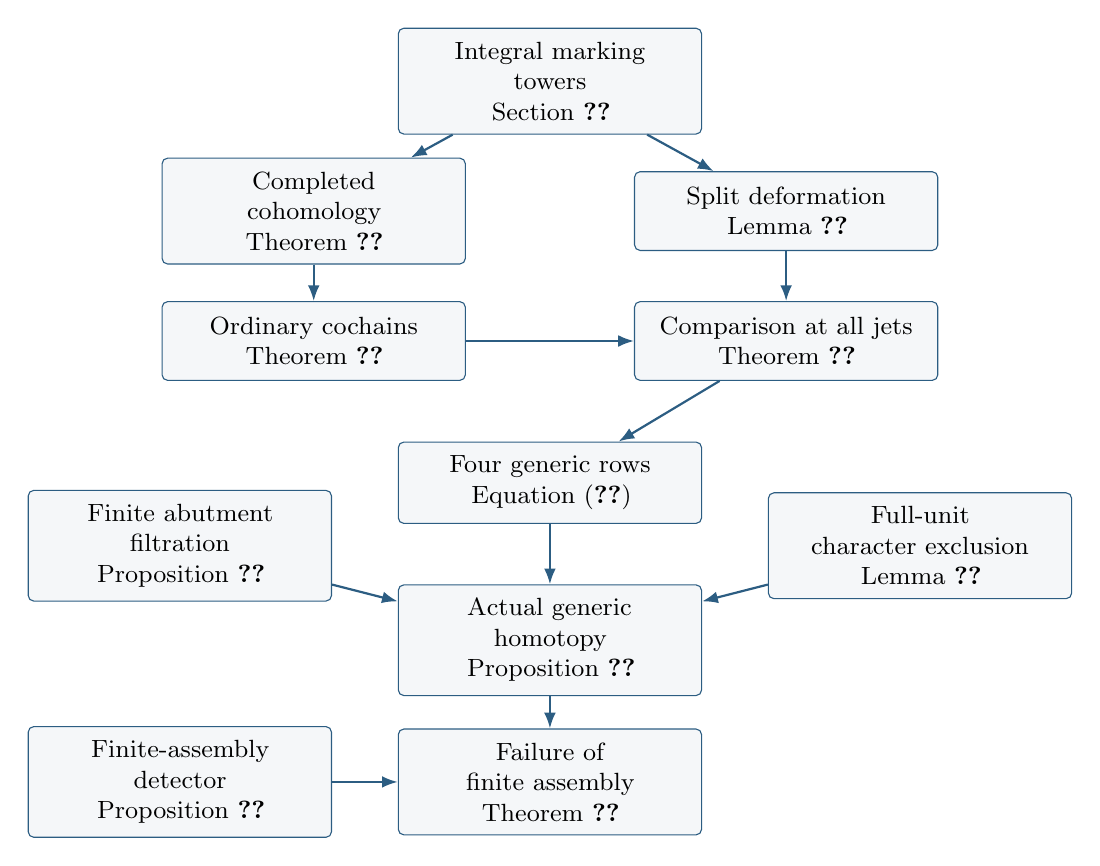
\begin{tikzpicture}[
  box/.style={draw=proofblue,rounded corners=2pt,fill=proofgray,
    align=center,text width=3.5cm,minimum height=1.0cm,
    inner sep=5pt,font=\small},
  arr/.style={-{Latex[length=2mm]},draw=proofblue,thick}
]
\node[box] (tower) at (0,0)
  {Integral marking\\towers\\Section~\ref{sec:towers}};
\node[box] (complete) at (-3,-1.65)
  {Completed\\cohomology\\Theorem~\ref{thm:completed-calculation}};
\node[box] (deform) at (3,-1.65)
  {Split deformation\\Lemma~\ref{lem:split-jet-lift}};
\node[box] (ordinary) at (-3,-3.3)
  {Ordinary cochains\\Theorem~\ref{thm:coefficient-calculation}};
\node[box] (jets) at (3,-3.3)
  {Comparison at all jets\\Theorem~\ref{thm:jet-comparison}};
\node[box] (page) at (0,-5.1)
  {Four generic rows\\Equation~\eqref{eq:obstruction-page}};
\node[box] (filtration) at (-4.7,-5.9)
  {Finite abutment\\filtration\\Proposition~\ref{prop:descent-test}};
\node[box] (units) at (4.7,-5.9)
  {Full-unit\\character exclusion\\Lemma~\ref{lem:generic-character}};
\node[box] (homotopy) at (0,-7.1)
  {Actual generic\\homotopy\\Proposition~\ref{prop:generic-homotopy}};
\node[box] (detector) at (-4.7,-8.9)
  {Finite-assembly\\detector\\Proposition~\ref{prop:constituent-test}};
\node[box] (failure) at (0,-8.9)
  {Failure of\\finite assembly\\Theorem~\ref{thm:main}};
\draw[arr] (tower) -- (complete);
\draw[arr] (tower) -- (deform);
\draw[arr] (complete) -- (ordinary);
\draw[arr] (deform) -- (jets);
\draw[arr] (ordinary) -- (jets);
\draw[arr] (jets) -- (page);
\draw[arr] (page) -- (homotopy);
\draw[arr] (filtration) -- (homotopy);
\draw[arr] (units) -- (homotopy);
\draw[arr] (homotopy) -- (failure);
\draw[arr] (detector) -- (failure);
\end{tikzpicture}
\caption{The coefficient comparisons and their passage to homotopy.
The full-unit action rules out differentials between the four generic
rows; the finite abutment filtration places their constituents in actual
homotopy. The finite-assembly detector then excludes the norm constituent.
Arrows indicate inputs to the next displayed stage.}
\label{fig:proof-chain}
\end{figure}

Section~\ref{sec:detector} proves the finite-construction test, and
Sections~\ref{sec:setup}--\ref{sec:towers} prepare the stage coefficients
and markings. Section~\ref{sec:finite-resolutions} supplies the finite
analytic resolution needed in Sections~\ref{sec:analytic}--\ref{sec:decompletion}.
Section~\ref{sec:homotopy} proves convergence and identifies the ordinary
cooperations, which Section~\ref{sec:jets} compares through every jet.
Section~\ref{sec:obstruction} completes the argument.
\FloatBarrier

\section{The finite-assembly detector}\label{sec:detector}

We first isolate the representation-theoretic condition imposed by a finite
construction from the \(K(2)\)-local unit. This condition will later be
tested on the abutment of the descent spectral sequence.

Throughout the proof, \(p=3\). Fix the finite field \(k\) chosen in the
introduction. Let \(\Gamma_i\) be the one-dimensional Honda formal group of
height \(i\), in a coordinate with \(p\)-series \(T^{p^i}\), and put
\[
 D_i=\End(\Gamma_i)[1/p],\qquad
 P_i=\Aut(\Gamma_i)=\mathcal O_{D_i}^{\times},\qquad J=P_2.
\]
The Honda endomorphism-order description gives the displayed unit group
\citep[Example~2.15]{BGHS22}.
These are the unextended stabilizer groups, so their actions fix \(k\).
Choose the unramified quadratic subfield \(F\subset D_2\), and set
\[
 G_F=\mathcal O_F^\times,\quad
 \mathcal O_x=k[[x]],\quad Q_x=k((x)),\quad
 \mathbf 1_2=L_{K(2)}S.
\]
The symbol \(G_F\) denotes this unit group, not an absolute Galois group.
Its action on \(\mathcal O_x\) extends to \(Q_x\).

Let \(E_2=E_2(k)\), with \(\pi_0E_2=W(k)[[x]]\). The marked-lift
stabilizer action on its coefficients is described in
\citet[Theorem~1.1 and Equation~(1.4)]{DH95}, and its Morava \(E\)-theory
realization is supplied by \citet[Corollaries~7.6--7.7]{GH04}.
We use the cotangent convention for its degree-two periodicity line,
dual to the degree-minus-two tangent convention in those sources:
\[
 \omega=\pi_2E_2,\qquad
 \Omega=\omega/p,\qquad
 \overline\omega=\Omega\otimes_{\mathcal O_x}Q_x.
\]
Thus \(\pi_{2j}E_2=\omega^{\otimes j}\) and odd homotopy vanishes. A
negative tensor power of a line means the corresponding power of its dual.
All these lines have their semilinear \(J\)-action. Unless a relative
product is explicitly indicated, \(\wedge\) denotes the ordinary smash
product of spectra.

\begin{lemma}[Reduction modulo \(p\)]\label{lem:mod-p-nullity}
Multiplication by \(p\) is null as an \(E_2\)-module map on \(E_2/p\).
For every spectrum \(X\), it therefore annihilates the homotopy groups of
\(L_{K(2)}(E_2\wedge X)/p\). Those groups are naturally
\(\mathcal O_x\)-modules.
\end{lemma}

\begin{proof}
Regularity of \(p\) and evenness of \(E_2\) give \(\pi_1(E_2/p)=0\).
Apply \([-,E_2/p]_{E_2}\) to the cofiber sequence for multiplication by
\(p\) on \(E_2\). Restriction along \(E_2\to E_2/p\) gives an injection
\[
 [E_2/p,E_2/p]_{E_2}\hookrightarrow\pi_0(E_2/p).
\]
The class \(p\id\) maps to zero and is therefore zero. Tensoring this null
map with \(X\) and applying exact localization proves the assertion. A
chosen \(J\)-equivariant nullhomotopy is not needed: the conclusion is the
nullity of the module map and the induced action on homotopy.
\end{proof}

For a spectrum \(X\), define
\begin{equation}\label{eq:generic-test}
 \mathcal T(X)=L_{K(2)}(E_2\wedge X)/p,
 \qquad
 \mathcal V_d(X)=\pi_d\mathcal T(X)\otimes_{\mathcal O_x}Q_x.
\end{equation}
The action comes from \(E_2\), so every map of underlying spectra induces
an equivariant map on this test. The action of \(G_F\) is semilinear:
\(g(av)=g(a)g(v)\) for \(a\in Q_x\) and \(v\in\mathcal V_d(X)\).
For a character \(\chi:G_F\to k^\times\), let \(Q_x(\chi)\) denote the
semilinear line with a basis \(e_\chi\) satisfying
\(g(e_\chi)=\chi(g)e_\chi\).

We use these representations algebraically. A subrepresentation is a
\(G_F\)-stable \(Q_x\)-linear subspace; no additional continuity condition
is imposed on that subspace. Every finite-dimensional semilinear
representation has finite length, because a strict chain of subspaces has
strictly increasing dimensions. Its simple constituents are therefore
well defined up to isomorphism and multiplicity.

\begin{proposition}[Constituents forced by finite assembly]
\label{prop:constituent-test}
Suppose that \(L_{K(2)}X\) belongs to the ordinary thick subcategory
generated by \(\mathbf 1_2\) in \(K(2)\)-local spectra. Then, for every
\(d\in\mathbb Z\), the representation \(\mathcal V_d(X)\) is
finite-dimensional over \(Q_x\), and each simple constituent is isomorphic
to \(\overline\omega^{\otimes b}\) for some \(b\in\mathbb Z\).
\end{proposition}

\begin{proof}
Let \(\mathcal A\) be the full subcategory of finite-dimensional semilinear
\(G_F\)-representations over \(Q_x\) whose simple constituents have the
indicated form. It is a Serre subcategory: subobjects and quotients retain
their constituents, and the constituents of an extension are those of its
two ends. It is also closed under finite sums and retracts.

The functor \(\mathcal T\) is exact. Localization of modules from
\(\mathcal O_x\) to \(Q_x\) is exact and respects the semilinear action.
An exact triangle \(X_1\to X_2\to X_3\) consequently gives an exact sequence
\[
 \mathcal V_d(X_1)\longrightarrow\mathcal V_d(X_2)
 \longrightarrow\mathcal V_d(X_3)
 \longrightarrow\mathcal V_{d-1}(X_1)
 \longrightarrow\mathcal V_{d-1}(X_2).
\]
If the terms arising from \(X_1\) and \(X_2\) lie in \(\mathcal A\) in
every degree, then \(\mathcal V_d(X_3)\) is an extension of a subobject of
\(\mathcal V_{d-1}(X_1)\) by a quotient of \(\mathcal V_d(X_2)\), and
hence also lies in \(\mathcal A\). Rotation gives the same assertion for
any choice of two terms. The condition is therefore closed under finite
sums, shifts, cofibers, and retracts.

For the local unit, \(\mathcal T(\mathbf 1_2)\simeq E_2/p\). Indeed,
\(S\to\mathbf 1_2\) is a \(K(2)\)-equivalence, tensoring with \(E_2\)
preserves \(K(2)\)-equivalences, and \(E_2\) is \(K(2)\)-local. Even
periodicity gives
\[
 \mathcal V_{2j}(\mathbf 1_2)=\overline\omega^{\otimes j},
 \qquad \mathcal V_{2j+1}(\mathbf 1_2)=0.
\]
The same observation shows that
\(\mathcal T(X)\simeq\mathcal T(L_{K(2)}X)\) for every \(X\). The condition
therefore holds on every object of the ordinary thick subcategory generated
by \(\mathbf 1_2\), and hence on \(X\) as stated.
\end{proof}

The Proposition proves finite dimensionality as well as the restriction on
constituents. It uses neither closure under tensoring with arbitrary
modules nor an identification of dualizable objects with objects in the
ordinary thick subcategory. To contradict it, the rest of the argument
will exhibit one actual simple subquotient that is not a periodicity power.

\section{Markings, coefficients, and conventions}\label{sec:setup}

The detector in Section~\ref{sec:detector} gives a condition that any finite
construction must satisfy. We now prepare the coefficient calculation that
will violate it. The prime remains \(p=3\), and \(k\) is the finite field
chosen there, containing \(\mathbb F_{p^6}\) and enlarged finitely when
needed to fix the constant identifications. Recall the Honda groups
\(\Gamma_i\), their division algebras \(D_i\), and their stabilizers
\(P_i=\mathcal O_{D_i}^{\times}\). The Honda forms can be chosen over
\(\mathbb F_p\), and their endomorphisms are defined over
\(\mathbb F_{p^i}\). Thus \(k\) contains both endomorphism fields needed
in heights two and three. Set
\begin{equation}\label{eq:stabilizers}
 P=P_3,\qquad
 H=\ker(\Nrd:P\longrightarrow\Zp^\times),\qquad
 J=P_2.
\end{equation}
The actions below are the unextended stabilizer actions: they fix \(k\).
When Galois descent is involved, it will be handled explicitly rather
than included silently in \(P\) or \(J\).

Choose the unramified quadratic subfield
\(F\subset D_2\). The character used in the obstruction is
\begin{equation}\label{eq:norm-character}
 \delta:\mathcal O_F^\times\longrightarrow\mathbb F_3^\times,
 \qquad
 \delta(g)=\overline{N_{F/\mathbb Q_3}(g)}.
\end{equation}
It is nontrivial because the residue-field norm
\(\mathbb F_9^\times\to\mathbb F_3^\times\) is surjective.
Its inverse and its unramified Galois conjugate are equal to it.

We also use
\[
 H'=\Nrd^{-1}(\mu_2),\qquad
 H'/H=\mu_2,\qquad
 P/H'\cong 1+3\mathbb Z_3\cong\mathbb Z_3.
\]
Here the reduced norm on maximal-order units is surjective. For these
particular algebras, one may see this on the units of an unramified
maximal subfield: the residue norm is surjective, and the norm on
principal units is surjective by the trace and the \(3\)-adic
logarithm. No group section of the full reduced norm is needed.

\subsection{The one-parameter stratum}

We first fix the coordinate normalization behind the Hasse coefficients.
Lubin--Tate construct a universal deformation from a normalized
representative of the special fibre \citep[Proposition~1.1, p.~50,
and Theorem~3.1]{LT66}. On the stratum where the preceding parameters
vanish, their parameter \(\tau_r\), with \(q=p^r\), occurs as
\[
 \Phi(X,Y)\equiv X+Y+\tau_r C_q(X,Y)
       \pmod{\text{total degree }q+1},
 \qquad
 C_q(X,Y)=\frac{(X+Y)^q-X^q-Y^q}{p}.
\]
The expression defining \(C_q\) is the integral polynomial used in
\citet[equations~(2.4)--(2.5), p.~256]{Lazard55}. Iterating the group
law \(p\) times and reducing in characteristic \(p\) gives
\[
 \begin{split}
 [p]_{\Phi}(T)
 &\equiv \tau_r\sum_{j=1}^{p-1} C_q(jT,T)\\
 &=\tau_r\frac{p^q-p}{p}T^q
  \equiv-\tau_r T^q\pmod{T^{q+1}}.
 \end{split}
\]
Thus the raw successive Hasse coefficient in that normalized
representative is \(-\tau_r\).

The Honda coordinate was already fixed in Section~\ref{sec:detector}.
Choose the special-fibre coordinate isomorphism from the normalized
representative to that Honda law and transport the universal family
along it. Write \(\lambda_h\in k^\times\) for its linear coefficient
in height \(h\). The normalization preceding Lubin--Tate Proposition~1.1
uses an isomorphism over the original residue field. Since the height-two
Honda law is defined over \(\mathbb F_9\), we perform that construction
already there, so \(\lambda_2\in\mathbb F_9^\times\). This transport makes the special fibre literally the
chosen Honda law, so its \(p\)-series is still \(T^{p^h}\). Under a
coordinate change \(T'=cT+O(T^2)\), the first nonzero coefficient at
\(T^{p^r}\) becomes \(c^{1-p^r}\) times the old coefficient. We
therefore name the height-three parameters
\[
 a=-\lambda_3^{1-p}\tau_1,\qquad
 t=-\lambda_3^{1-p^2}\tau_2,
\]
and name the height-two parameter
\(x=-\lambda_2^{1-p}\tau_1\). These are unit rescalings of regular
parameters. In the transported families the first raw Hasse
coefficient is exactly \(a\), the next one modulo \(a\) is exactly
\(t\), and the first height-two coefficient is exactly \(x\). These
are chosen coordinate normalizations, rather than identities
independent of a coordinate. In the Lubin--Tate representative itself
they read \(a=-\tau_1\), \(t=-\tau_2\), and \(x=-\tau_1\).

We choose the mixed-characteristic height-two parameter compatibly.
Lift the chosen height-two coordinate isomorphism coefficientwise to
\(W(\mathbb F_9)\); its linear coefficient remains a unit. Transport the
mixed-characteristic Lubin--Tate family along this lift. The resulting
family over \(W(\mathbb F_9)[[\tau_1]]\) has a regular
parameter lifting this \(x\): multiply \(\tau_1\) by a lift of the
nonzero constant \(-\lambda_2^{1-p}\). We denote the lift by \(x\) as
well and use the scalar-extended family over \(W(k)[[x]]\) for \(E_2(k)\).
Functorial Morava \(E\)-theory realization
\citep[Section~7 and Corollary~7.7]{GH04} supplies the map from
\(E_2(\mathbb F_9)\) to \(E_2(k)\); its coefficient map sends the chosen
regular parameter \(x\) to \(x\). This convention will be
used in the completion comparison in Section~\ref{sec:homotopy}.

Let
\[
                    A=k[[a,t]]
\]
be the universal equal-characteristic deformation ring of
\(\Gamma_3\) in this normalization \citep[Theorem~3.1]{LT66}.
Let \(\mathcal G\) denote the associated algebraic \(p\)-divisible
group over \(A\).

We specify the order of construction, since it matters after \(t\)
is inverted. The formal multiplication-by-\(p^r\) series over \(A\)
is distinguished of degree \(p^{3r}\).
Weierstrass preparation gives its finite flat kernel over \(A\);
the formal group law supplies its group structure. These kernels,
with their compatible inclusions, form \(\mathcal G\).
This is the finite-torsion construction over a complete local base in
\citet[Section~2.2, Proposition~1]{Tate67}.
This equivalence also transfers universality to the algebraic family.
Let \(B\) be a complete Noetherian local \(k\)-algebra with residue field
\(k\), and let \(H/B\) be a marked deformation of
\(\Gamma_3[p^\infty]\). For \(Q_r=\mathcal O(H[p^r])\), the algebra
\[
 Q_r/\mathfrak m_BQ_r\cong k[T]/(T^{p^{3r}})
\]
is local. Since \(Q_r\) is finite over \(B\), every maximal ideal lies
over \(\mathfrak m_B\), so \(Q_r\) is local and \(H\) is connected in
Tate's sense. The inverse equivalence gives a formal group of dimension
one, as on the closed fibre; a coordinate lifting the marking makes it
a Lubin--Tate deformation. Full faithfulness identifies its marked isomorphisms
\citep[Section~2.2, Proposition~1, and Section~2.3]{Tate67}.
The prepared finite kernels commute with local base change. Hence
Lubin--Tate universality transfers to the above algebraic
\(\mathcal G/A\), supplying the universality used by the later
Kodaira--Spencer argument \citep[Theorem~3.1 and paragraph~3.2]{LT66}.
We then pull this finite torsion system back along
\[
                    A\longrightarrow K=k((t)),\qquad a\longmapsto0.
\]
On this stratum the \(p\)-series factors through the
\(p^2\)-power Frobenius, and the remaining homomorphism has invertible
linear coefficient \(t\). Thus \(\mathcal G_K\) has a connected
part of height two and an \'etale quotient of height one.
Forming only the formal completion at the identity after this base
change would discard the latter quotient.

The ring-theoretic differential statement needed later is elementary
in these coordinates.

\begin{lemma}\label{lem:finite-p-basis}
The ordinary module \(\Omega^1_{A/k}\) is free on \(da,dt\) and agrees
with the module of continuous differentials.
The element \(t\) is a \(p\)-basis of \(K\), remains a \(p\)-basis at
each finite separable field extension of \(K\), and gives
\(\Omega^1_{L/k}=L\,dt\) for the marking algebra defined below.
\end{lemma}

\begin{proof}
Since \(k\) is perfect, every \(f\in A\) has a unique expansion
\[
          f=\sum_{0\leq i,j<p}a^it^j f_{ij}^{\,p},
          \qquad f_{ij}\in A.
\]
Ordinary derivations therefore have the usual partial-derivative
formula and are determined freely by the values of \(a,t\).
The continuous partial derivatives show that these values are
independent. This proves the assertion for \(A\).
The corresponding one-variable expansion proves the assertion for
\(K\). A \(p\)-basis is preserved by a separable algebraic extension:
Frobenius base change along a separable extension is an isomorphism,
so the basis of \(K\) over \(K^p\) remains a basis after that base
change. The differential statement follows by the same argument.
For a finite \'etale algebra it holds on each field factor, and it
passes to the filtered union defining \(L\).
\end{proof}

The universal deformation theory of \(p\)-divisible groups gives a
functorial Kodaira--Spencer isomorphism over \(A\)
\citep[Section~5]{Lau10}; the version over
arbitrary square-zero target rings is recalled where it is used in
Proposition~\ref{prop:invariant-differential} and
Theorem~\ref{thm:jet-comparison}.
Lemma~\ref{lem:finite-p-basis} explains why the ordinary algebraic
differentials in that theorem are available after specializing to
the Laurent field \(K\).

\subsection{The connected marking tower}

The connected-marking tower is the coheight-one construction studied by
Gross and Torii \citep[Theorem~3.5(1a)]{Gross79}
\citep[Section~2.3 and Theorem~2.9]{Torii03}. In Torii's Laurent-field
setting the lower-height stabilizer acts simply transitively on markings
and commutes with the higher-height action. We use the ind-\'etale torsor
form, allowing products of fields at finite stages, and prove the integral
\'etale marking and finite-level descent needed below.

Let \(L\) be the algebra classifying isomorphisms between the
connected formal law of \(\mathcal G_K\) and the constant Honda
formal group \(\Gamma_2\). Its coefficient construction and
separability are proved in Section~\ref{sec:towers}. The marking
space is a pro-\'etale torsor under the pro-constant group \(J\).
We write
\begin{equation}\label{eq:marking-algebra}
          L=\colim_{U\subset J} L^U ,
\end{equation}
where \(U\) runs through open subgroups and \(L^U\) is the finite
\'etale \(K\)-algebra of markings modulo \(U\).
The superscript is compatible with the \(J\)-action on the tower.
The finite stages need not be fields.

The height-three stabilizer \(P\) acts on the universal deformation and
preserves its height strata \citep[Proposition~3.3 and paragraph~3.4]{LT66}.
It also transports a connected marking.
Changes of the connected marking give the commuting \(J\)-action.
Thus \(P\) preserves each \(L^U\), while \(J\) carries stages to
the corresponding conjugate stages.
The actions on finite jets and their \'etale lifts are continuous.
Normalize the valuation of \(K\) by \(v(t)=1\), extend it to each
field factor of \(L^U\), and give a product of factors its product
topology. The \(P\)-action preserves these valuations, since its
action on the height-two stratum takes \(t\) to a unit multiple of
\(t\).

For a finite stage \(B=L^U\), put
\[
 B_e=B^{1/p^e},\qquad
 B^{\mathrm{perf}}=\bigcup_{e\geq0}B_e,\qquad
 B^\flat=\widehat{B^{\mathrm{perf}}}.
\]
Roots are taken inside the perfection and all valuations are
extended from \(B\). Each \(B_e\) is complete. The symbol \(B^\flat\)
in this paper means the \emph{completed perfection of this finite
stage}; it does not denote the completion of the entire marking
tower. The other perfection used throughout the proof is
\[
                         R=L^{\mathrm{perf}}
                          =\colim_{U,e}(L^U)^{1/p^e}.
\]
These conventions are applied factorwise to products of fields.

\subsection{Continuous cochains at finite stages}

We use inhomogeneous continuous group cochains. If a compact group
\(Q\) acts continuously on a complete coefficient module \(M\), then
\(C^s_{\mathrm{cts}}(Q,M)=
\operatorname{Map}_{\mathrm{cts}}(Q^s,M)\), with the usual bar
differential. An extra compact profinite parameter space \(T\)
means
\[
 C^s_{\mathrm{cts}}(Q,M;T)
       =\operatorname{Map}_{\mathrm{cts}}(T\times Q^s,M);
\]
the differential leaves \(T\) fixed.
The parameter space need not be metrizable.

\begin{definition}[Stage cochains]\label{def:stage-cochains}
For \(Q=P,H,H'\), or a closed subgroup of one of these groups,
cochains with the incomplete coefficients \(L\) and \(R\) mean
\begin{align}
 C^s_{\mathrm{cts}}(Q,L;T)
   &:=\colim_U
       \operatorname{Map}_{\mathrm{cts}}(T\times Q^s,L^U),
       \nonumber\\
 C^s_{\mathrm{cts}}(Q,R;T)
   &:=\colim_{U,e}
       \operatorname{Map}_{\mathrm{cts}}
            (T\times Q^s,(L^U)^{1/p^e}).
       \label{eq:stage-cochains}
\end{align}
We also use the completed-stage complex
\begin{equation}\label{eq:completed-stage-cochains}
 \colim_U C^\bullet_{\mathrm{cts}}(Q,(L^U)^\flat;T).
\end{equation}
All filtered colimits in these definitions are taken degreewise.
Omitting \(T\) means that \(T\) is a point.
\end{definition}

Thus each element of one of the complexes in
Definition~\ref{def:stage-cochains} has its values in a single complete
finite marking or root stage. We do not identify this convention
with all continuous maps into an incompletely topologized union.
The algebraic inclusion \(L\to R\), and the inclusions of finite
root stages into their completed perfections, give natural maps
between these complexes. They retain the \(P\)- and \(J\)-actions
on the full directed systems. A proof may restrict to cofinally
many stages containing specified finite data; the maps themselves
are defined before that restriction.

The use of parameters is part of each comparison theorem below.
It supplies the iterated cochains for quotient descent and the
continuous function coefficients of Morava cooperations. On a
discrete target, compactness makes continuous functions locally
constant with finite image. On a complete valuation target it
instead gives uniform approximation on finite clopen partitions;
the distinction will be used in
Section~\ref{sec:decompletion}.

\subsection{Geometric notation}

For a perfectoid base in characteristic \(p\), let \(V_i\) denote
the basic vector bundle of rank \(i\) and degree one on the
relative Fargues--Fontaine curve. The notation
\[
                  N=H^1(V_2^\vee),\qquad N^*=N\setminus\{0\}
\]
means the associated cohomology sheaf and its complement of the
zero section on the relevant \(v\)-site.
Relative section-sheaf statements, rather than just statements
about individual geometric fibers, will be used in
Section~\ref{sec:towers}. Over an algebraically closed perfectoid
field \(C^\flat\), a choice of untilt \(C\) gives the concrete
presentation of \(N^*\) used for the analytic calculation.
Base Frobenius is defined before this choice.

The height-two Morava theory and its periodicity line used by the homotopy
test were fixed in Section~\ref{sec:detector}. The height-three theory
will enter after the ordinary coefficient calculation is complete.

\section{The marking towers and their determinant normalization}
\label{sec:towers}

The calculation uses two kinds of marking on the height-two stratum of a
height-three deformation.  A connected marking identifies its formal group
with a Honda group.  An \emph{integral} étale marking chooses a generator of
the Tate module of its étale quotient.  The distinction matters: the first
has structure group $J=\mathcal O_{D_2}^{\times}$, whereas the automorphism
group of the corresponding vector bundle is $D_2^{\times}$.
Theorem~\ref{thm:two-towers} gives the quotient comparison;
Lemmas~\ref{lem:etale-marking} and~\ref{lem:lift-torsors} retain its
normalized integral marking and identify the lift algebras.
In this section write $G=\mathcal G$ for the algebraic $p$-divisible
group fixed in Section~\ref{sec:setup}.

Put
\[
 d=p^2,\qquad q=p^3,\qquad A_2=A/(a)=k[[t]].
\]
We use Honda coordinates in which $[p]_{\Gamma_i}(T)=T^{p^i}$.
For an affinoid perfectoid $k$-algebra $(C,C^+)$, let
\[
 \mathcal H_i(C,C^+)=C^{\circ\circ},
\]
with addition given by $\Gamma_i$.  Since $C$ is perfect and $[p]$ is the
$p^i$-power map, $\mathcal H_i$ is a sheaf of $\Qp$-vector spaces.
All complements of zero in this section mean nonzero on every geometric
fiber.  The arguments below concern the characteristic-$p$ perfectoid
site over $k$.

\subsection{Finite torsion algebras}

We first retain the entire $p$-divisible group $G$, including the part that
becomes étale after $t$ is inverted.  Its finite kernels are formed over
$A$ by Weierstrass preparation and then base changed.  Thus, on $A_2$,
the algebra of $G[p^l]$ is the prepared finite algebra of $[p^l](T)$;
it has rank $p^{3l}$.  Formal completion at the identity is not taken
after passage to $K$.

\begin{lemma}[Primitive torsion coordinates]
\label{lem:primitive-coordinates}
For $l\geq 1$, let $\mathcal B_l$ be the reduced closure, over $A_2$,
of the points of $G[p^l]_K$ whose images generate the étale quotient.
Write $s_l$ for its point coordinate and set
$s_j=[p^{l-j}](s_l)$ for $1\leq j\leq l$.  Then
\begin{equation}
 \mathcal B_l=k[[s_l]],\qquad
 \mathcal C_l:=k[[t]][s_l^{d^l}]=k[[s_l^{d^l}]].
 \label{eq:primitive-rings}
\end{equation}
The algebra $\mathcal C_l[1/t]$ is the finite étale algebra of generators
of $G_K^{\mathrm{et}}[p^l]$.  Over it, the algebra of \emph{all} lifts of
the universal generator is $\mathcal B_l[1/t]$, finite free of rank $d^l$.
The transition maps are finite and injective, and
\begin{equation}
 s_j\in k[[s_l^{d^{l-j}}]]\qquad(l\geq j).
 \label{eq:primitive-transitions}
\end{equation}
\end{lemma}

\begin{proof}
Define the closure as the image of the finite $A_2$-algebra of $p^l$-torsion
in the reduced generic algebra of the indicated primitive locus.  It is
finite and reduced, every component dominates $\Spec A_2$, and its
closed fiber is supported at $s_l=0$.  It is therefore a complete local
ring with residue field $k$, dimension one, and maximal ideal $(t,s_l)$.
The element $s_1$ is nonzero on every generic component.

The series $[p](T)$ factors through $T^d$, and its reduction at $t=0$
is $T^q$.  Its coefficient of $T^d$ is $t$.  Dividing $[p](s_1)=0$
by $s_1^d$ in the reduced generic algebra gives
\[
 t\,u(s_1^d,t)+s_1^{q-d}=0,
 \qquad u(0,t)=1.
\]
Here $u$ is a unit power series.  This identity holds in the closure by
generic density.  It also holds in the complete finite subalgebra
$\mathcal C_l$: the series for $[p^{l-1}]$ factors through
$T^{d^{l-1}}$, so $s_1^d$ is a series in $t$ and $s_l^{d^l}$ with
zero constant term in the latter variable.  Since $q-d\geq d$, the
identity puts $t$ in the ideal $(s_l^{d^l})$ of $\mathcal C_l$.
Its maximal ideal is consequently generated by $s_l^{d^l}$.
Its dimension is one because it is integral over $A_2$.
The surjection
$k[[W]]\twoheadrightarrow\mathcal C_l$, $W\mapsto s_l^{d^l}$,
is an isomorphism: a nonzero ideal in $k[[W]]$ would lower dimension.
The same argument, now with generator $s_l$, proves the first identity
in \eqref{eq:primitive-rings}.  These are identifications of the
inclusion $\mathcal C_l\subset\mathcal B_l$, not just abstract
regularity assertions.

Write $[p^l](T)=g_l(T^{d^l})$ and prepare $g_l$.
The linear coefficient of $g_l$ is a unit multiple of
$t^{1+d+\cdots+d^{l-1}}$.  The invariant-differential identity for this
Frobenius-divided homomorphism shows that its derivative, in its prepared
kernel algebra, is that coefficient times a unit.  After inverting $t$
the prepared algebra is therefore étale, of rank $p^l$.
Its kernel before dividing by Frobenius has connected rank $d^l$.
The primitive images are distinguished exactly by $s_l^{d^l}$, so
their generator algebra is $\mathcal C_l[1/t]$.

The scheme of lifts of this generator is finite locally free of rank
$d^l$.  Its coordinate algebra surjects onto
$\mathcal B_l[1/t]$ by the same point coordinate.  But
\eqref{eq:primitive-rings} makes the latter free of rank $d^l$ over
$\mathcal C_l[1/t]$, with basis $1,s_l,\ldots,s_l^{d^l-1}$.
The surjection is an isomorphism.  In particular, reduction in the
definition of the closure has not removed any infinitesimal part of the
lift scheme on the exact-height locus.

Every primitive étale generator at level $j$ lifts at level $l$ after
a geometric extension.  The generic transition is consequently
surjective on spectra and injective on the reduced coordinate algebras;
generic density gives injectivity on the closures.  The transition is
finite because $\mathcal B_l$ is finite over $A_2$.  Finally,
$[p^{l-j}](T)$ factors through $T^{d^{l-j}}$.  Substituting the expression
for $t$ in $k[[s_l^{d^l}]]$ proves
\eqref{eq:primitive-transitions}.
\end{proof}

The connected marking algebra $L$ has a different construction.
Height classification gives an isomorphism of the formal law of
$G_K$ with $\Gamma_2$ over an algebraic closure
\cite[Theorem~IV]{Lazard55}.  In fact its coefficients are separable
over $K$.  Write the isomorphism as $f(T)=\sum_{n\geq1}b_nT^n$
and compare $f([p](T))=f(T)^d$.  At degree $nd$ this gives
\[
 b_n^d-t^n b_n=Q_n(b_1,\ldots,b_{n-1}),
\]
where $Q_n$ has coefficients in $K$.  This polynomial in $b_n$
has derivative $-t^n\ne0$.  The first equation is
$b_1^{d-1}=t$ with $b_1\ne0$.  Induction puts every coefficient
in a finite separable extension, so the entire isomorphism is
defined over a separable closure.  Its inverse has the same
property.  These successive finite separable coefficient equations,
with the formal-law identities imposed, construct the isomorphism
torsor by finite étale jet algebras.  Its automorphisms are the
constant Honda group $J$.  Thus
\[
 L=\colim_{U\subset J}L^U
\]
is an ind-étale $J$-torsor over $K$, with $U$ ranging over open subgroups.
This also gives the exact-height marking description recalled in
Section~\ref{sec:setup}; see the coheight-one marking
algebra in \cite[Section~2.7]{BMR26}.  Finite products of fields are
allowed at each stage.  The action of $P$ transports the deformation and
its connected marking, and the action of $J$ changes that marking.
They commute, fix $k$, and preserve the valuation normalized by $v(t)=1$.
In particular every $L^U$ is $P$-stable.  All actions on finite
coefficient data are continuous for the valuation topology.

\subsection{The normalized coordinate limit}

The following explicit comparison will also ensure that the frame
identification is integral.  Let $G_t$ be a specialization of the formal
law on $A_2$ to an affinoid perfectoid $k$-algebra $(C,C^+)$, with
$t\in C^{\circ\circ}$.  Write $P_t(T)=[p]_{G_t}(T)$.

\begin{lemma}[Universal-cover coordinates]
\label{lem:cover-coordinates}
There is a natural additive isomorphism
\[
 \Phi_t:\mathcal H_3(C,C^+)\xrightarrow{\ \sim\ }
 \varprojlim_{[p]}G_t(C^{\circ\circ}).
\]
Its coordinates and inverse are
\begin{equation}
 \Phi_t(z)_j=\lim_{r\longrightarrow\infty}
      P_t^{\circ r}\bigl(z^{1/q^{j+r}}\bigr),
 \qquad
 \Phi_t^{-1}((b_j))=\lim_{j\longrightarrow\infty}b_j^{q^j}.
 \label{eq:cover-limit}
\end{equation}
The isomorphism is $\Qp$-linear and is compatible with coefficient
maps and changes of deformation frame.  On an algebraically closed
perfectoid field, the zeroth projection is surjective and its kernel
is the integral Tate module of $G_t^{\mathrm{et}}$.
\end{lemma}

\begin{proof}
Use the spectral norm and choose $\lambda<1$ bounding $|t|$.
The coefficients of $P_t(T)-T^q$ and of $G_t-\Gamma_3$ have norm at
most $\lambda$.  Integral power series are $1$-Lipschitz on the open
unit ball, and factorization through $T^d$ gives
\begin{equation}
 |P_t^{\circ r}(v)-P_t^{\circ r}(w)|
       \leq |v-w|^{d^r}.
 \label{eq:cover-contraction}
\end{equation}
Successive approximations in the first formula in
\eqref{eq:cover-limit} differ by at most $\lambda^{d^r}$.
They therefore converge; their limits are topologically nilpotent and
satisfy
\[
 |\Phi_t(z)_j-z^{1/q^j}|\leq\lambda,
 \qquad P_t(\Phi_t(z)_{j+1})=\Phi_t(z)_j.
\]
For a compatible sequence $(b_j)$, consecutive normalized coordinates
differ by at most $\lambda^{q^j}$.  Hence its displayed inverse exists
and satisfies
\[
 |z-b_j^{q^j}|\leq\lambda^{q^j}.
\]
After taking the relevant root this error is at most $\lambda$;
applying \eqref{eq:cover-contraction} makes it tend to zero.
This proves one inverse identity.  Raising the first displayed
estimate to $q^j$ proves the other.  No common upper bound strictly
less than one for all the individual $|b_j|$ is required.

The coefficients of $\Gamma_3$ are fixed by $q$-power Frobenius.
The discrepancy between the specialized addition law and the Honda
addition law is bounded by $\lambda$; after normalization, or after
$r$ applications of $P_t$, it tends to zero by the same estimates.
Thus the formulas respect addition.  A change of deformation frame
differs from its Honda reduction by topologically small coefficients.
Its Honda reduction commutes with $q$-power Frobenius, since its
coefficients lie in $\mathbb F_{p^3}$.  The identical estimate proves
frame equivariance.  The maps commute with integral multiplication
and with inverse multiplication by $p$, so are $\Qp$-linear.
Continuity, including continuous scalar families, follows from uniform
convergence on smaller balls.

Over an algebraically closed field, preparation applied to
$P_t(T)-w$ gives a monic polynomial whose roots are small whenever
$w$ is small.  Choosing roots successively proves surjectivity of the
zeroth projection.  Its kernel consists of compatible $p^j$-torsion
points.  Connected finite groups have only the identity as a point
over a perfect field, so this kernel is precisely the Tate module of
the étale quotient.
\end{proof}

Let $X$ be the completed perfection of the punctured formal $t$-disc,
equivalently $\Spa(K^\flat)$.  Let $\mathcal T_{\mathrm{et}}\to X$ be the tower
of integral étale Tate generators.  By
Lemma~\ref{lem:primitive-coordinates}, it is the perfected inverse
tower of the primitive-coordinate spaces on $t\ne0$.

\begin{proposition}[Comparison of the entire generator tower]
\label{prop:generator-ball}
There is a natural $P\times\Zp^\times$-equivariant isomorphism
\begin{equation}
 \mathcal T_{\mathrm{et}}\simeq\mathcal H_3\setminus\{0\},
 \qquad (s_l)\longmapsto z=\lim_l s_l^{q^l}.
 \label{eq:generator-ball}
\end{equation}
It identifies completed function algebras, with their spectral norms,
on an exhaustion by smaller closed balls.  The assertion commutes
with base change and remains valid after adjoining any compact
profinite parameter space.
\end{proposition}

\begin{proof}
Retain the reduced closures from
Lemma~\ref{lem:primitive-coordinates}, including their point at $t=0$.
After perfection, a point of the étale quotient has a unique lift
through the connected factor.  The resulting inverse tower is thus
the tower of the rings $\mathcal B_l$.

We check its complete algebras after extension to an algebraically
closed perfectoid field $C$ of characteristic $p$.  Fix
$0<\rho<1$ in its value group and put $y_l=s_l^{q^l}$.
At level $l$ take the closed disc $|y_l|\leq\rho$.
At a point of this disc, write $\lambda=|t|$.
The proof of Lemma~\ref{lem:primitive-coordinates} at level one,
and finite telescoping of normalized coordinates, give
\[
 \lambda\leq |s_1|^d,
 \qquad |s_1|\leq\max(\rho^{1/q},\lambda).
\]
If $\lambda>\rho^{1/q}$ these inequalities would imply
$0<\lambda\leq\lambda^d<\lambda$.  Consequently
\begin{equation}
 \lambda\leq\rho^{d/q},\qquad
 |y_{l+1}-y_l|\leq\lambda^{q^l}
                   \leq\rho^{d q^{l-1}}<\rho.
 \label{eq:generator-radius}
\end{equation}
The finite transition maps preserve these discs.  Conversely, every
geometric point of a level-$l$ disc has a lift by finite surjectivity,
and the strict inequality in \eqref{eq:generator-radius} forces its
lifts to remain in the next disc.  Pullback is therefore isometric
for the spectral norm, also after completed perfection.

In the completion of the direct limit of these perfected Gauss
algebras, $y_l$ converges to $z$.  Send the coordinate of the perfected
radius-$\rho$ disc to $z$.  The resulting homomorphism is isometric:
for a polynomial in finitely many fractional powers, evaluation at
$y_l$ has exactly its Gauss norm, since $s_l$ is a free disc
coordinate and $q^l$ is a power of $p$.  These evaluations converge
to evaluation at $z$.  For a nonzero polynomial, their difference
is eventually smaller than its fixed norm, so the limiting norm is
the same.  Completion preserves this isometry.

The image is dense.  For $l\geq j$, write
$s_j=F_{j,l}(s_l^{d^{l-j}})$ as in
\eqref{eq:primitive-transitions}, with $F_{j,l}\in k[[T]]$.
Replacing $s_l$ by $z^{1/q^l}$ changes this expression by at most
\[
 \lambda^{d^{l-j}}\leq\rho^{(d/q)d^{l-j}},
\]
which tends to zero with $l$.  The substituted series converges on
the $z$-disc.  The same approximation after taking roots proves
that every $s_j$ and each of its $p$-power roots belongs to the
closed image.  These generate the completed limit algebra.
The isometry is therefore onto.

Here is the relative descent explicitly.  Let
$E=\widehat{k((u))^{\mathrm{perf}}}$, with $u$ an auxiliary
variable, and choose $C=\widehat{\overline E}$.
For an affinoid perfectoid test $S=\Spa(A,A^+)$, a
pseudouniformizer $\pi\in A^+$ and its unique compatible roots
give a continuous map $E\to A$, $u\mapsto\pi$.
The field extension $\Spa(C,C^\circ)\to\Spa(E,E^\circ)$ is
a $v$-cover, so its base change
\[
 S_C=S\times_{\Spa(E,E^\circ)}\Spa(C,C^\circ)\longrightarrow S
\]
is a $v$-cover.  The calculation over $C$ established an
isomorphism of complete algebras, hence of perfectoid spaces,
on every smaller disc.  It therefore applies to all $C$-tests,
including $S_C$, rather than only to geometric points.
The coordinate map is defined over $k$; its inverse over this
cover is unique and agrees on the \v Cech overlap, so it descends
to $S$.  This uses base change of an established isomorphism,
not preservation of a spectral isometry by an arbitrary
completed tensor product.  Smaller discs exhaust the comparison:
on a quasicompact test $t$ is uniformly small, and the first
torsion coordinate and \eqref{eq:generator-radius} bound all
normalized coordinates uniformly away from radius one.

It remains to identify the puncture.  If $z=0$ on a geometric fiber,
Lemma~\ref{lem:cover-coordinates} gives $|s_l|\leq\lambda$ for all
$l$.  For fixed $j$,
\[
 |s_j|=|P_t^{\circ(l-j)}(s_l)|
           \leq\lambda^{d^{l-j}}\longrightarrow0.
\]
Thus all $s_j$ vanish, and the primitive-coordinate equation forces
$t=0$.  Conversely, at $t=0$ the reduced torsion coordinates vanish.
Removing these corresponding zero loci gives
\eqref{eq:generator-ball}.  Equivariance is the frame and scalar
equivariance of Lemma~\ref{lem:cover-coordinates}.
Every estimate used a uniform spectral norm; taking the supremum
over a compact profinite parameter preserves each estimate and each
density argument.
\end{proof}

\subsection{Relative bundles and integral frames}

We spell out the vector-bundle results used in the comparison.
For a perfectoid test $S$, write $X_S$ for its relative
Fargues--Fontaine curve.  Relative cohomology means the associated
sheaf on the $v$-site; it does not posit a morphism of schemes
$X_S\to S$.  The bundles $V_i$ are the Honda forms of rank $i$
and degree one.

\begin{lemma}[Relative section facts]
\label{lem:relative-section-facts}
There are natural isomorphisms of additive sheaves
\[
 \mathcal H_i\simeq \mathcal H^0(V_i),\qquad
 \mathcal H^0(\mathcal O)=\underline{\Qp}.
\]
The automorphism sheaf of $V_i$ is the locally profinite group
$D_i^\times$.  A family fiberwise isomorphic to $V_i$ is locally
of that form on the perfectoid site.  Trivial bundles and these
positive basic bundles have no higher relative cohomology sheaves.
For such bundles, $\underline{\Qp}$-linear maps between the section
sheaves are exactly the maps of bundles, relatively and compatibly
with base change.
\end{lemma}

\begin{proof}
The Lubin--Tate universal-cover description of sections of
$\mathcal O(1)$ is
\cite[Proposition~II.2.2]{FS21}.  Applying it with the unramified
coefficient field of degree $i$ and pushing forward gives
$\mathcal O(1/i)=V_i$ and the Honda height-$i$ cover.
The positive-section calculation, including the perfected-ball
description, is also
\cite[Proposition~II.2.5]{FS21}.
The classification on geometric curves and the relative pure-family
theorem give the stated local forms and automorphisms; see
\cite[Theorems~II.2.14 and II.2.19]{FS21}.
Equivalently, the basic stratum is the classifying stack of the
corresponding division-algebra group
\cite[Theorem~III.4.5]{FS21}.
The Honda forms are defined over our $k$: commuting with
$[p](T)=T^{p^i}$ puts every coefficient of a geometric Honda
endomorphism in $\mathbb F_{p^i}\subset k$.

For precision about maps, let $\tau$ denote the morphism of sites
used for relative curve cohomology.  Ansch\"utz--Le~Bras prove that
\[
 R\tau_*:\Perf(X_S)\longrightarrow
 D(S_v,\underline{\Qp})
\]
is fully faithful for every small $v$-stack $S$
\cite[Corollary~3.11]{ALB25}.
The same section calculation gives
$R\tau_*\mathcal O=\underline{\Qp}$ and
$R\tau_*V_i=\tau_*V_i[0]$; the latter uses positivity.
Taking degree-zero morphisms in this fully faithful functor proves
the last assertion.  These statements are relative on $S$, so they
apply over the finite-field base site and to forms obtained by
descent.  In particular, the assertion about $\mathcal O$ is
vanishing of its higher \emph{relative sheaves}, not an assertion
of vanishing on every unrefined test object.
\end{proof}

\begin{lemma}[The two stable-bundle tests]
\label{lem:stable-bundle-tests}
A section of $V_3$ nonzero on every geometric fiber gives a
subbundle $\mathcal O\hookrightarrow V_3$ with quotient locally
isomorphic to $V_2$.  Conversely, an extension
\begin{equation}
 0\longrightarrow\mathcal O\longrightarrow E
       \longrightarrow V_2\longrightarrow0
 \label{eq:basic-extension}
\end{equation}
has middle bundle fiberwise $V_3$ if and only if its extension class
is nonzero on every geometric fiber.  Moreover,
$\mathcal H^0(V_2^\vee)=0$.
\end{lemma}

\begin{proof}
Work first on a geometric curve.  The saturation of the image of a
nonzero section $\mathcal O\to V_3$ is a line bundle of nonnegative
integral degree.  Stability of $V_3$ bounds that degree by $1/3$,
so it is zero.  The section has no zeros, since a nonzero effective
divisor has positive degree.  Its quotient has rank two and degree
one.  A quotient of that quotient of nonpositive slope would also
be a quotient of $V_3$, contrary to semistability.  Its slopes are
therefore positive.  The classification of vector bundles, and
integrality of the degree of each stable summand, force the
quotient to be $V_2$.

An extension \eqref{eq:basic-extension} has no negative-slope
quotient, since neither end has a nonzero map to a negative-slope
bundle.  If it has a slope-zero quotient, that quotient receives
a nonzero map from the kernel $\mathcal O$, because
$\Hom(V_2,\mathcal O)=0$.  The quotient is a sum of copies of
$\mathcal O$; compose with a linear functional nonzero on that
kernel image and rescale.  This gives a retraction onto the
kernel, so the extension splits.  A nonsplit
extension thus has only positive slopes.  A positive bundle of
rank three and degree one can have only the stable type $V_3$.
The converse is immediate from stability.  The asserted vanishing
is the negative-slope section vanishing.

These arguments use the degree and slope classification on a
geometric Fargues--Fontaine curve
\cite[Proposition~II.2.10 and Theorem~II.2.14]{FS21}.
Fiberwise surjectivity is the relative subbundle condition; the
local forms in Lemma~\ref{lem:relative-section-facts} and descent
give the corresponding relative statements.
\end{proof}

Let
\[
 \widetilde X=\varprojlim_U\Spa((L^U)^\flat)
\]
be the perfected completed connected-marking tower.  This notation
does not replace the finite-stage coefficient convention of
Definition~\ref{def:stage-cochains} by cochains on a completion of
the whole tower.

\begin{proposition}[Integral frame comparison]
\label{prop:integral-frames}
There exists a determinant identification
$\iota:\det V_3\xrightarrow{\sim}\det V_2$ over $k$
for which the following conclusions hold.  Fix such an identification
for the sequel.  There is an isomorphism
\begin{equation}
 \widetilde X\simeq\operatorname{Surj}(V_3,V_2).
 \label{eq:connected-surjections}
\end{equation}
A surjection has a unique kernel frame for which its determinant
identification is $\iota$.  Under
\eqref{eq:connected-surjections}, this is an integral étale Tate
generator for the corresponding deformation.
The source-frame group $P$ acts by reduced norm on this normalization,
and a target-frame change in $J$ has its corresponding constant
determinant adjustment.
\end{proposition}

\begin{proof}
We construct the quotient frame, normalize its determinant, and then
recover the markings from an arbitrary surjection.  The reconstruction
will show that every surjection arises from an integral connected marking.

\smallskip\noindent\emph{Constructing the quotient frame.}
Over $\mathcal T_{\mathrm{et}}$, Proposition~\ref{prop:generator-ball} identifies
the chosen Tate generator with a nonzero section
$\mathcal O\to V_3$.  After adding a connected marking, there is
also a quotient frame.  To construct it, orient the formal marking
as an isomorphism from the specialized formal law to $\Gamma_2$.
Its coefficients are bounded by one on perfectoid tests.  Indeed,
its leading coefficient has norm $|t|^{1/(d-1)}<1$, and the same
coefficient comparison gives
$b_n^d-t^n b_n=Q_n(b_1,\ldots,b_{n-1})$ with integral coefficients.
If all earlier coefficients have norm at most one, a root with
$|b_n|>1$ would make the monic term strictly larger than every
other term.  Induction gives the assertion.

Consequently the formal marking can be evaluated on all small
points.  Compose it with the zeroth projection in
Lemma~\ref{lem:cover-coordinates}.  This gives an additive map
$\mathcal H_3\to\mathcal H_2$.  It is $\Qp$-linear because
multiplication by $p$ is invertible on the Honda target.  It kills
the Tate generator and hence its $\Qp$-span.  By
Lemma~\ref{lem:relative-section-facts} it comes from a unique
bundle map $V_3\to V_2$.  On a geometric fiber this map is nonzero:
near the origin the formal marking has nonzero linear coefficient,
and the zeroth projection is surjective.

Lemma~\ref{lem:stable-bundle-tests} identifies the quotient by the
Tate section with $V_2$ locally.  The induced nonzero endomorphism
of this quotient is invertible, since its endomorphism algebra is
the division algebra $D_2$.  The resulting quotient frame is
therefore an isomorphism, also relatively.  Uniqueness in relative
full faithfulness makes the construction equivariant and compatible
with all base changes.

\smallskip\noindent\emph{Normalizing the determinant.}
An initial determinant identification $\iota_0$ exists over $k$.
In the cyclic
Honda isocrystal the determinant Frobenius differs from the
rank-one degree-one isocrystal by the cyclic permutation sign
$(-1)^{i-1}$.  The possible minus sign is removed over
$\mathbb F_{p^2}$ by a Teichm\"uller unit $u$ with $u^p=-u$.
Our field contains $\mathbb F_{p^6}$, so the required identifications
are defined over $k$.  Automorphisms act on these determinant
lines by their reduced norms.

Connected markings form a $J$-torsor over $\mathcal T_{\mathrm{et}}$ and change
the quotient frames through precisely $J$.  On this torsor define
the determinant isomorphism and its discrepancy by
\begin{align*}
 \Delta(e,f)(e\wedge v_2\wedge v_3)&=f(v_2)\wedge f(v_3),\\
 r(e,f)&=\Delta(e,f)\iota_0^{-1}\in\underline{\Qp^\times}.
\end{align*}
Changing the marking by $j\in J$ multiplies $r$ by
$\Nrd(j)\in\Zp^\times$.  Consequently
$\nu=v_p(r)$ descends through this torsor to a locally constant
function $\mathcal T_{\mathrm{et}}\to\underline{\mathbb Z}$.
After extension to the field $C$ used in
Proposition~\ref{prop:generator-ball}, the space $\mathcal T_{\mathrm{et},C}$
is a punctured perfected open disc.  Nested connected closed
annuli exhaust it, and perfection preserves their topology;
thus $\nu_C$ is a single integer $m$.
The covers $S_C\to S$ constructed there also show that
$\Spa(C,C^\circ)\to\operatorname{Spd}(k)$ is $v$-surjective.
Hence $\mathcal T_{\mathrm{et},C}\to\mathcal T_{\mathrm{et}}$ is a $v$-cover and
$\nu=m$ descends globally.  Set $\iota=p^m\iota_0$.
The new discrepancy is $p^{-m}r$ and is everywhere a unit.

Each pair of connected and étale markings therefore gives an exact
sequence
\[
 0\longrightarrow\mathcal O\longrightarrow V_3
       \longrightarrow V_2\longrightarrow0
\]
whose determinant identification is a unit multiple of $\iota$.
For a fixed connected marking, multiply its étale generator by this
unit to obtain determinant equality.  There is exactly one such
generator; uniqueness glues it over $\widetilde X$.  We have thus
constructed a map from $\widetilde X$ to $\operatorname{Surj}(V_3,V_2)$,
with a determinant-normalized integral kernel frame.

\smallskip\noindent\emph{Recovering the markings.}
To prove that this map is an isomorphism, start with an arbitrary
surjection $f:V_3\twoheadrightarrow V_2$.  Determinant equality supplies
its kernel generator $e_f$.  Proposition~\ref{prop:generator-ball}
reconstructs from $e_f$ a deformation and a primitive integral
Tate generator.  Choose a connected marking locally and let $f_0$
be the quotient frame it constructs.  Write $f=b f_0$ with
$b\in D_2^\times$.  Put $r_0=\Delta(e_f,f_0)\iota^{-1}$,
which is a unit by the normalization above.  Since
$\Delta(e_f,f)=\iota$, we have $1=\Nrd(b)r_0$.  Thus
$v_p(\Nrd b)=0$, so $b\in J$ and the required change of marking
is integral.  It is unique because the marking torsor and the
integral quotient-frame torsor have the same group $J$.
Indeed, replacing the local marking by $j$ replaces $f_0$ by
$jf_0$ and $b$ by $bj^{-1}$, so the adjusted markings agree
and glue.  The resulting connected marking maps back to $f$.
Conversely, starting with a connected marking,
Proposition~\ref{prop:generator-ball} recovers its deformation from the
normalized integral generator, and the $J$-torsor uniqueness recovers
its marking.  These constructions commute with base change,
so they prove the relative isomorphism \eqref{eq:connected-surjections}.
In particular, the normalized kernel frame of every surjection is
the integral Tate generator of its reconstructed deformation.

A $p$-power rescaling of $e_f$ can change the reconstructed
deformation; the coordinate comparison still returns a primitive
basis for that deformation.  No primitivity claim about the old
deformation is needed.

\smallskip\noindent\emph{The frame actions.}
The actions can be recorded without an implicit choice of a section
of the norm map.  In the frame convention
\[
 (g,j)\cdot f=j f g^{-1},\qquad(g,j)\in P\times J,
\]
the normalized kernel frame satisfies
\begin{equation}
 e_{jfg^{-1}}=\Nrd(j)\Nrd(g)^{-1}\,g e_f.
 \label{eq:normalized-frame-action}
\end{equation}
This is the determinant identity for the exact sequence.  Reversing
all frame conventions inverts the displayed norm characters.
In either convention $H$ fixes the normalized étale frame under
transport, and the $P$ and $J$ adjustments are continuous constant
units.
\end{proof}

Put $N=\mathcal H^1(V_2^\vee)$, the relative sheaf of extensions of
$V_2$ by $\mathcal O$, with both ends framed.

\begin{lemma}[Finite marking stages of the perfected tower]
\label{lem:perfected-marking-torsor}
For each open $U\subset J$, the map
\[
 \widetilde X\longrightarrow\Spa(B^\flat),\qquad B=L^U,
\]
is a pro-étale $U$-torsor.  It is natural in $U$, in coefficient
base change, and in the commuting $P$-action.  The space
$\widetilde X$ is represented by the completed perfection of the
whole algebraic marking tower, equipped with its uniform valuation
norm; this representation is used here only to discuss its geometry.
\end{lemma}

\begin{proof}
For $V\triangleleft U$ open, $L^V/L^U$ is a finite étale
$U/V$-torsor.  Perfection commutes with finite étale base change.
After completion it remains the finite étale torsor
\[
 \Spa((L^V)^\flat)\longrightarrow\Spa(B^\flat).
\]
One may check the completed algebra explicitly in a finite field
basis: completion of its scalar extension from $B^{\mathrm{perf}}$
is $(L^V)^\flat$, since finite-dimensional valued spaces are
complete and their norms are equivalent to the coordinate norms.
This works componentwise for field products and preserves the
torsor identities.

The completed direct limit of these perfected finite-stage
algebras is uniform, perfect, and Tate, with the common
pseudouniformizer $t$.  It is therefore perfectoid.  Its associated
space is their affinoid inverse limit.  The finite-level torsor
identities pass to this limit and identify its relation with
$\underline U\times\widetilde X$.
Surjectivity can be checked on a geometric point of $\Spa(B^\flat)$:
choose compatible lifts through the surjective finite étale
covers, using compactness of their finite fibers, and extend the
resulting bounded map to the completion.  This also proves the
covering assertion.  Every construction commutes with restrictions
and the transported $P$-action.
\end{proof}

\begin{theorem}[The determinant-one two-tower comparison]
\label{thm:two-towers}
For each open $U\subset J$ and $B=L^U$ there is a natural equivalence
of $v$-stacks over $k$
\begin{equation}
 [\Spa(B^\flat)/H]\simeq[N^*/U].
 \label{eq:two-towers}
\end{equation}
It is obtained from the commuting torsor presentations
\[
 \widetilde X/U\simeq\Spa(B^\flat),\qquad
 \widetilde X/H\simeq N^*.
\]
The residual group $P/H=\Zp^\times$ acts on $N^*$ by kernel
scalars through reduced norm, up to the common inverse convention.
The $J$-action changes the quotient frame and makes the kernel
determinant adjustment in
\eqref{eq:normalized-frame-action}.  All these identifications
commute with base change and products with profinite parameter spaces.
\end{theorem}

\begin{proof}
By Proposition~\ref{prop:integral-frames}, $\widetilde X$ is the
space of surjections $V_3\to V_2$ with their uniquely normalized
kernel frames.  Quotienting the middle frame by $H$ allows the
middle bundle to vary while preserving its determinant frame.
Lemma~\ref{lem:stable-bundle-tests} identifies precisely the
resulting objects with the nowhere-split extensions of $V_2$ by
$\mathcal O$, namely $N^*$.  There is no automorphism group left
over an extension with its two ends fixed, since
$\mathcal H^0(V_2^\vee)=0$.

To see that this is a torsor presentation relatively, first choose
a local basic frame of the middle bundle.  Its determinant frame
can be corrected to the prescribed one: reduced norm
$D_3^\times\to\Qp^\times$ is surjective.  The compatible frames
form a torsor under its norm-one subgroup, which is exactly $H$,
because norm one has valuation zero.  On units, surjectivity of
$P\to\Zp^\times$ already follows from the norm of the maximal
unramified cubic subfield.  Local basic triviality then gives the
asserted $H$-torsor on the site.

Combine it with the $U$-torsor in
Lemma~\ref{lem:perfected-marking-torsor}.  The actions commute, so
the two iterated quotient presentations give
\eqref{eq:two-towers}.  Tracking determinants gives the claimed
actions.  For example, in the frame convention of
\eqref{eq:normalized-frame-action}, the residual $g\in P$ acts
on extension classes by the scalar $\Nrd(g)$; a target change
$j$ acts by pullback along $j^{-1}$ together with kernel scalar
$\Nrd(j)^{-1}$.  This states the actual action and does not choose
a group-theoretic splitting of reduced norm.  Naturality and the
parameter assertion follow from the natural torsor maps and the
uniform coordinate comparison.
\end{proof}

\subsection{Descent of the integral marking}

The normalized generator has so far been constructed on a completed
perfected tower.  We next descend each of its finite étale levels to
the algebraic marking algebra $L$.  The following elementary lemma
is the completion statement needed for this purpose.

\begin{lemma}[Finite étale sections descend]
\label{lem:finite-etale-descent}
Let $L=\colim_i B_i$ be an injective union of finite étale
$K$-algebras, with their maximum valuation norms, and let
$C=\widehat{L^{\mathrm{perf}}}$.  For every finite étale
$L$-algebra $E$, the map
\[
 \Hom_{L\text{-alg}}(E,L)\longrightarrow
 \Hom_{L\text{-alg}}(E,C)
\]
is bijective.  Each section on the right is defined at a finite
separable stage.  The assertion allows unbounded numbers of field
factors among the $B_i$.
\end{lemma}

\begin{proof}
Each $B_i^{1/p^r}$ is a finite product of complete valued fields.
First let $e\in C$ be an idempotent.  Approximate it by
$b\in B_i^{1/p^r}$ with $\lVert b-e\rVert<1$.
Then $\lVert b^2-b\rVert<1$ and $2b-1$ is a unit with inverse
of norm at most one.  Hensel's lemma in that complete finite
product gives an idempotent $e_i$ at distance less than one from
$e$.  Two such idempotents are equal: both $e(1-e_i)$ and
$e_i(1-e)$ are idempotents of norm less than one, hence zero.
Purely inseparable extensions create no idempotents, so $e=e_i$
belongs to $B_i$.  Finitely many idempotents descend to a common
stage.

The algebra $E$ descends to a finite étale algebra over some $B_i$.
After a finite idempotent partition it has a monogenic étale
presentation; each component field of $B_i$ is infinite, so the
primitive-element argument applies also to its finite étale
products.  Descend the idempotents selected by the proposed
section.  It remains to descend finitely many simple roots.

Let $f(z)=0$ with $f\in B_i[T]$ and $f'(z)$ invertible in $C$.
Approximate $z$ and $f'(z)^{-1}$ simultaneously by $b,c$ in a
single $B_j^{1/p^r}$, so closely that
\[
 \lVert1-cf'(b)\rVert<1.
\]
The geometric series in this complete algebra makes $f'(b)$
invertible with inverse norm at most $\lVert c\rVert$.
Let $M\geq1$ bound the quadratic Taylor remainder of $f$ on
the unit ball about $b$, and put $C_0=\max(1,\lVert c\rVert)$.
The approximations may also be chosen so that
\[
 \lVert f(b)\rVert C_0^2M<1.
\]
Newton iteration remains in $B_j^{1/p^r}$, has uniformly bounded
inverse derivatives, and converges there to a root $z_j$.
Choose the initial approximation inside a simple-root uniqueness
ball about $z$; the divided difference is a unit on that ball,
so $z_j=z$.  Componentwise, this root is separable over $B_j$
but belongs to its purely inseparable extension, and hence was
already in $B_j$.  All the finitely many roots use a common
stage.  This proves surjectivity, and injectivity follows from
$L\hookrightarrow C$.
\end{proof}

\begin{lemma}[The normalized algebraic étale marking]
\label{lem:etale-marking}
The étale quotient of $G_L$ has a compatible integral Tate
generator defined over $L$, obtained by determinant normalization.
It is fixed by $H$.  Transport by $P$ changes it by the constant
reduced-norm unit, up to the common inverse convention; transport
by $J$ has the constant determinant adjustment determined by
\eqref{eq:normalized-frame-action}.  Each finite torsion level
of this marking is defined at a finite separable marking stage.
\end{lemma}

\begin{proof}
The integral Tate frame constructed in
Proposition~\ref{prop:integral-frames} gives, at each level $l$,
a section of the finite étale generator algebra of
$G_L^{\mathrm{et}}[p^l]$ after passage to
$\widehat{L^{\mathrm{perf}}}$.
Lemma~\ref{lem:finite-etale-descent} descends this section to
some finite separable marking stage.  The descended sections
are compatible: their transition identities hold in the
completion and hence in $L$ by injectivity.  The same argument
descends the action identities, including the $H$-invariance.
The finite stage can depend on $l$; no single finite stage
containing the entire Tate generator is required.
\end{proof}

\begin{lemma}[The generator-lift torsors]
\label{lem:lift-torsors}
The scheme of lifts in $G_L[p^l]$ of the normalized étale
generator has coordinate algebra
\begin{equation}
 R_l=L^{1/p^{2l}}=L^{1/d^l}\subset R=L^{\mathrm{perf}}.
 \label{eq:lift-rings}
\end{equation}
It is a torsor under the marked group $\Gamma_2[p^l]_L$.
The transition maps give the indicated inclusions inside $R$.
The action of $H$ commutes with translation by this constant
group.  The other frame actions conjugate translations by
continuous constant Honda automorphisms and scalar norm units.
All coactions and their finite-level action identities are
defined and continuous after passage to a sufficiently large
finite separable stage.
\end{lemma}

\begin{proof}
The fiber over the marked étale generator is a torsor for the
connected kernel.  The connected marking identifies that
kernel with $\Gamma_2[p^l]$.
By Lemma~\ref{lem:primitive-coordinates}, its algebra before
base change along the chosen generator is
\[
 k[[s_l]][1/t]
 \quad\text{over}\quad
 k[[s_l^{d^l}]][1/t],
\]
and this is the full lift algebra of rank $d^l$.
The generator marking of Lemma~\ref{lem:etale-marking}
gives its base change to $L$.

Every finite separable extension of $K$ has one-element
$p$-basis $t$, and the same is true of their ind-étale union.
A finite purely inseparable extension of degree $d^l$ in
its perfection is therefore $L^{1/d^l}$.  The displayed lift
algebra retains that degree after the separable base change:
componentwise, $s_l^{d^l}$ is a $p$-basis of its Laurent-series
field and remains a $p$-basis after any separable extension.
This proves \eqref{eq:lift-rings}, also for products by a
common finite-stage argument.  Purely inseparable embeddings
are unique, so compatibility of the marked generators
identifies the transition maps with the inclusions inside $R$.

The group $H$ fixes both the connected frame and the normalized
étale generator.  Its transported action on each lift torsor
therefore commutes with translations in the named Honda group.
For the remaining actions, transport followed by restoration
of the normalized étale generator rescales by its constant
norm unit; changing the connected frame also applies the named
Honda automorphism.  These are continuous constant group
automorphisms and satisfy the action identities because the
markings do.  At a fixed level all these statements involve
finite torsion algebras and finitely many coefficients.  Those
coefficients lie in a finite separable stage, and the resulting
maps between complete finite-dimensional valued spaces are
continuous.  Enlarging that stage handles any specified finite
list of levels and identities.

For later use, the order-two action has a direct sign check.
The central elements $\tau=-1\in P$ and $j=-1\in J$ both act
on surjections by $f\mapsto-f$.  Since $V_2$ has rank two,
$\Delta(e,-f)=\Delta(e,f)$, so the normalized generator $e$,
its reconstructed deformation, and its étale frame are unchanged.
The connected marking $\phi$ is replaced by $-\phi$.
A translation labeled by $c\in\Gamma_2[p^l]$ uses
$\phi^{-1}(c)$; after this change it uses $\phi^{-1}(-c)$.
Thus $\tau$, whose reduced norm is $-1$, conjugates the named
translation group by $[-1]$.  Its action on the one-dimensional
tangent of the Cartier dual is $-1$, as required in
Lemma~\ref{lem:distribution-operator}.
\end{proof}

\subsection{The negative period space}

The final geometric description will be used to compute cohomology.
It requires a geometric untilt only after the space and its frame
actions have been defined over $k$.

\begin{lemma}[An untilt presentation of the negative space]
\label{lem:negative-presentation}
Let $C^\flat$ be an algebraically closed perfectoid field of
characteristic $p$ containing $k$, choose an algebraically closed
untilt $C/\mathbb C_p$, and let $F/\Qp$ be unramified quadratic.
After choosing its embedding at the untilt divisor there are
isomorphisms
\begin{equation}
 N_{C^\flat}\simeq
       (\mathbb G_{a,C})^\diamond/\underline F,
 \qquad
 (N^*)_{C^\flat}\simeq
       [ (\mathbb A^1_C\setminus\underline F)^\diamond/
          \underline F].
 \label{eq:negative-presentation}
\end{equation}
Here $\mathbb A^1_C$ is the analytic affine line.  In the second
expression the $F$-support is removed fiberwise
before taking the translation quotient.  The action of
$F^\times$ through the quotient frame is multiplication in this
presentation, up to inversion and the choice of unramified
embedding.  The additional kernel determinant adjustment
from Theorem~\ref{thm:two-towers} is a scalar in $\Zp^\times$.
\end{lemma}

\begin{proof}
On the Fargues--Fontaine curve with coefficient field $F$,
the chosen untilt divisor gives \citep[Proposition~II.2.3]{FS21}
\[
 0\longrightarrow\mathcal O_F(-1)
  \longrightarrow\mathcal O_F
  \longrightarrow i_*C\longrightarrow0.
\]
The degree-zero section sheaf of $\mathcal O_F$ is
$\underline F$, its higher relative cohomology sheaves vanish,
and the negative line has no sections.  The cohomology sequence
therefore identifies
\[
 \mathcal H^1(\mathcal O_F(-1))
       \simeq (\mathbb G_{a,C})^\diamond/\underline F.
\]
Finite pushforward along the unramified coefficient extension
takes $\mathcal O_F(-1)$ to $V_2^\vee$, giving the first
isomorphism.  The preimage of the zero extension class is
exactly the sheaf $\underline F$.  Its complement consists
precisely of classes nonzero on every geometric fiber, proving
the second isomorphism as an open subquotient.

The sequence is equivariant for multiplication by $F^\times$.
The embedding and frame conventions may conjugate or invert
this action.  The independent determinant normalization of
the kernel contributes exactly the scalar described in
Theorem~\ref{thm:two-towers}.  For later use, a scalar
$u\in\Zp^\times$ has norm $u^2$ in $F/\Qp$, which is
trivial modulo $3$; thus this adjustment does not change the
nontrivial residue-norm character on $\mathcal O_F^\times$.
\end{proof}

The two-tower comparison and its normalized scalar action now supply the
geometric input for the completed calculation. Before using them, we
establish the finite analytic resolution that controls continuous cochains.

\section{Finite resolutions for the analytic groups}
\label{sec:finite-resolutions}

The completed coefficient calculation uses continuous cohomology with
noncompact valuation coefficients. We first give the finite resolution
that computes those cochains and bounds their cohomological degrees.
This tool depends only on the analytic groups and coefficient topology.
A linearly topologized \(\Fp\)-space is understood to be separated; an
action has \emph{invariant neighborhoods} when invariant open linear
subspaces form a neighborhood basis of zero.

\begin{lemma}[Finite analytic resolutions]
\label{lem:finite-resolution}
Let $G$ be a compact $p$-adic analytic group with no element of order $p$,
and put $d=\dim G$.  The trivial module $\Fp$ admits a length-$d$
resolution $Q_\bullet$ by finitely generated projective
$\Fp[[G]]$-modules, with their compact topologies.  If $M$ is a complete
linearly topologized $\Fp$-representation with invariant neighborhoods,
then
\[
 \Hom_{\Fp[[G]],\mathrm{cts}}(Q_\bullet,M)
 \simeq \Ccts(G,M)
\]
by continuous chain-homotopy equivalences.  Each term on the left is a
continuous direct summand of a finite power of $M$.

For $G=H$ the dimension is eight, and the reversed group-ring dual of
$Q_\bullet$ resolves the trivial right $\Fp[[H]]$-module.  In particular,
continuous $H$-cohomology of these coefficients vanishes above degree
eight, and finite coefficient modules have finite cohomology.
\end{lemma}

\begin{proof}
We specify the two structural inputs.  A completed group algebra over
$\Zp$, or over its residue field, is Noetherian; it has finite global
dimension when the compact analytic group has no element of order $p$
\cite[Section~3.3, Proposition~(d),(e)]{AW06}.  Also
\begin{equation}
 \label{eq:analytic-dualizing-cohomology}
 H^a_{\mathrm{cts}}(G,\Zp[[G]])=
 \begin{cases}
  \mathcal D_G,&a=d,\\
  0,&a\ne d,
 \end{cases}
\end{equation}
where $\mathcal D_G$ is free of rank one over $\Zp$, with the right
action given by the top exterior power of the dual adjoint
representation \cite[Proposition~4.16, Remark~4.23, and
Proposition~4.40]{BGHS22}.

Set $\widetilde\Lambda=\Zp[[G]]$ and $\Lambda=\Fp[[G]]$.
Noetherianity and finite global dimension give a finite resolution of
$\Zp$ by finitely generated projective $\widetilde\Lambda$-modules.
Give every term its topology as a summand of a finite power of
$\widetilde\Lambda$.  The differentials are continuous and their images
are compact, hence closed.  All syzygies are $p$-torsion-free, so
reduction modulo $p$ remains exact and gives a finite projective
$\Lambda$-resolution of $\Fp$.

Here the integral projective resolution computes
\eqref{eq:analytic-dualizing-cohomology} as continuous cohomology.
Indeed, a completed free $\Zp$-module on a profinite set is compact and
$p$-torsion-free.  Its Pontryagin dual is a divisible discrete
$p$-primary group, and hence injective.  It is therefore projective in
compact $\Zp$-modules.  Induction to $\widetilde\Lambda$ shows that the
completed bar terms are projective in compact
$\widetilde\Lambda$-modules.  The usual projective comparison maps and
homotopies can consequently be chosen continuous.  Dualizing the finite
integral resolution and then reducing modulo $p$ gives cohomology
$\mathcal D_G/p$ in degree $d$ alone: both the integral terms and the
unique integral cohomology module are $p$-torsion-free.  Finite
projectivity identifies this reduction with the group-ring dual of the
reduced resolution.  If its last degree is $n>d$, the last differential
of that dual surjects onto a projective module.  Split this surjection
and dualize back to remove a contractible pair.  Repetition gives a
resolution of length $d$.

We explain why the same compact resolution works for the possibly
noncompact target $M$.  For a profinite space $Z$, there is a natural
identification
\begin{equation}
 \label{eq:completed-free-continuous-functions}
 C_{\mathrm{cts}}(Z,M)
 =\Hom_{\Fp,\mathrm{cts}}(\Fp[[Z]],M).
\end{equation}
Modulo each open linear subspace of $M$, a continuous function has
finite image and factors through a finite clopen partition of $Z$.
Its linear extension therefore exists in that quotient.  The extensions
are compatible, and completeness gives the required map into $M$.
This also proves uniqueness.  With invariant neighborhoods the
$G$-action extends continuously to $\Lambda$.

The completed $\Fp$-bar terms are projective in compact
$\Lambda$-modules.  To lift a map from their profinite generators across
a compact-module surjection, first choose a continuous linear section
of the underlying compact $\Fp$-spaces.  Such a section exists by
dualizing and splitting an injection of discrete vector spaces.
Extend the lifted generator map $\Lambda$-linearly using
\eqref{eq:completed-free-continuous-functions}.  Thus the completed bar
resolution and $Q_\bullet$ are continuously chain-homotopy equivalent.
Apply continuous $\Lambda$-linear Hom into $M$.  Continuity of the
resulting maps and homotopies for the uniform cochain topologies is
checked modulo invariant open subspaces of $M$.  Finally, finite
projectivity makes each Hom term a continuous summand of $M^r$ for
some finite $r$.

For $H$, an element of order three would embed
$\mathbb Q_3(\zeta_3)$ in the division algebra $D_3$.  The degree of a
commutative subfield divides the degree three of this central division
algebra, whereas $[\mathbb Q_3(\zeta_3):\mathbb Q_3]=2$.  Thus $H$ has
no element of order three.  Its Lie algebra is the kernel of reduced
trace on $D_3$, so it has dimension eight.  Over a splitting field,
conjugation on $D_3$ becomes conjugation on $M_3$ and has determinant
one.  The decomposition
\[
 D_3=\Qp\cdot1\oplus\ker(\operatorname{Trd})
\]
is valid over $\Qp$, including at $p=3$, and the first summand has
trivial action.  The adjoint determinant on $\Lie(H)$ is therefore one.
Consequently $\mathcal D_H$ is the trivial line, which proves the
assertion about the reversed dual.  The remaining statements follow
by applying the finite resolution.
\end{proof}

For the torsion-free uniform open subgroups of \(J\), the same lemma
applies with dimension four. For \(H\), it supplies the dimension-eight
resolution and duality orientation needed later in the finite-stage
argument. We now turn to the completed geometric coefficients.

\section{The completed cohomology calculation}
\label{sec:analytic}

The goal is the completed coefficient calculation in
Theorem~\ref{thm:completed-calculation}.  We first compute the geometric
cohomology and its actions, then descend Frobenius at each finite marking
stage and take the marking colimit.  Throughout this section, \(C\) is an
algebraically closed complete perfectoid extension of \(\mathbb C_p\),
with a chosen embedding \(k\hookrightarrow C^\flat\).  On diamonds over
\(C^\flat\) we write \(\mathcal O^\flat\) for the characteristic-\(p\)
structure sheaf.  Thus, on the diamond of a perfectoid space in
characteristic \(p\), this is its usual structure sheaf; on an untilted
analytic space it is the structure sheaf on its characteristic-\(p\)
perfectoid site.

Let \(T\) be an arbitrary compact profinite set.  Products with \(T\)
always mean products with its associated locally profinite v-sheaf.
For a complete topological coefficient group \(M\), put
\[
 C^r_{\mathrm{cts}}(G,M;T)
   =\operatorname{Map}_{\mathrm{cts}}(T\times G^r,M).
\]
When \(G\) is compact and \(M\) is a Banach space, this mapping space has
the supremum norm.  For a Fr\'echet space it has the supremum seminorms
of a countable family of Banach seminorms.  Products indexed by a
discrete set have their product topology; they carry no boundedness
condition across that discrete set.  These conventions will be
preserved throughout the calculations.

\subsection{Two facts about continuous families and countable limits}

We first record the approximation argument used in the analytic
exhaustions.

\begin{samepage}
\begin{lemma}
\label{lem:analytic-roos}
Let
\[
 M_0 \xleftarrow{f_0} M_1 \xleftarrow{f_1} M_2
       \xleftarrow{} \cdots
\]
be a countable inverse system of complete nonarchimedean normed
abelian groups.  Suppose every \(f_n\) is a contraction with dense
image.  Then the map
\begin{equation}
 \prod_{n\geq0}M_n\longrightarrow\prod_{n\geq0}M_n,\qquad
 (x_n)\longmapsto(x_n-f_n(x_{n+1}))
 \label{eq:analytic-roos}
\end{equation}
is surjective.  The same assertion holds after replacing every \(M_n\)
by \(\operatorname{Map}_{\mathrm{cts}}(T,M_n)\).
Consequently these systems have no positive derived inverse limits.
\end{lemma}
\end{samepage}

\begin{proof}
Fix a right-hand side \((y_n)\) and positive real numbers
\(\varepsilon_n\to0\).  Suppose that a finite tuple
\(x_0,\ldots,x_n\) solves the first \(n\) equations.  By density choose
\(x_{n+1}\) such that
\[
 d_n=y_n+f_n(x_{n+1})-x_n,\qquad \|d_n\|<\varepsilon_n.
\]
Replace \(x_n\) by \(x_n+d_n\), and replace each earlier \(x_i\) by
\[
 x_i+f_i f_{i+1}\cdots f_{n-1}(d_n).
\]
The enlarged tuple now solves the first \(n+1\) equations.  Each
previously chosen coordinate has changed by at most
\(\varepsilon_n\).  Starting with any \(x_0\), this procedure produces
a Cauchy sequence in every fixed coordinate.  Completeness gives a
solution of all equations.

For the parameter assertion, the mapping spaces are complete and
the induced maps are contractions.  They have dense image: a
continuous map from \(T\) to \(M_n\) is uniformly approximated by a map
constant on a finite clopen partition, and its finitely many values
can be approximated in the image of \(M_{n+1}\).  Apply the preceding
argument to these mapping spaces.  Finally, the two-term Roos
complex \eqref{eq:analytic-roos} computes the derived inverse limit
of a countable system.
\end{proof}

The \(c_0\)-condition on a weighted coefficient family means that,
for every \(\varepsilon>0\), only finitely many weighted coefficient
norms are at least \(\varepsilon\).
We use two other elementary consequences of compactness.  First, a
continuous map from \(T\) to a weighted \(c_0\)-space has uniformly
small tails.  Indeed, its compact image admits a finite cover by
small balls, and the finitely many centers have uniformly small
tails.  Conversely, continuous coordinate functions with uniformly
small tails define a continuous map into that \(c_0\)-space.  Applying
this observation to each seminorm gives its Fr\'echet version.
Second, if \(V\) is discrete, every continuous map \(T\to V\) has
finite image.  In particular, continuous \(V\)-valued functions lift
through every surjection of discrete groups, by choosing lifts on
a finite clopen partition.

For use with Kummer covers, continuous cohomology of
\(\mathbb Z_p\) on a complete, separated, linearly topologized
\(\Fp\)-module \(M\) with invariant neighborhoods is computed by
\begin{equation}
 [\,M\xrightarrow{\gamma-1}M\,],
 \label{eq:analytic-cyclic}
\end{equation}
in degrees \(0,1\), where \(\gamma\) is a topological generator.
Here one applies continuous \(\Hom\) to
\[
 0\longrightarrow\Fp[[\mathbb Z_p]]
 \xrightarrow{\gamma-1}\Fp[[\mathbb Z_p]]
 \longrightarrow\Fp\longrightarrow0.
\]
This finite resolution compares continuously with the completed bar
resolution.  To check the assertion for the possibly noncompact
target \(M\), reduce modulo an invariant open subspace: a continuous
map from a profinite set then has finite image and extends linearly
to the free compact \(\Fp\)-module on that set.  Taking the inverse
limit over the open subspaces recovers \(M\) by completeness.
The same argument applies to
\(\operatorname{Map}_{\mathrm{cts}}(T,M)\), or directly to bar
cochains with parameter \(T\).  The finite analytic resolutions used
below have the same comparison property; see
Lemma~\ref{lem:finite-resolution} in
Section~\ref{sec:finite-resolutions}.

\subsection{Kummer annuli and the affine line}

Choose a compatible system of \(p\)-power roots of unity in \(C\).
It determines \(\epsilon\in C^\flat\) and a generator \(\gamma\) of
the Kummer group \(\mathbb Z_p(1)\).  Put
\(\theta=|\epsilon-1|\), so \(0<\theta<1\).
Let \(0<r\leq b\) belong to the value group of \(C\), and let
\(A[r,b]\) be the untilted closed annulus with coordinate \(z\).
We use the perfectoid coordinate-root construction and tilting
equivalence of \cite[Propositions~5.20 and~6.17]{Scholze12}.
After adjoining all \(p\)-power roots of \(z\), the perfectoid
Kummer cover has tilted function algebra
\begin{equation}
 \mathcal A[r,b]
 =
 \left\{\sum_{u\in\mathbb Z[1/p]}c_u z^u:
 \bigl(|c_u|\max(r^u,b^u)\bigr)_u\text{ is }c_0\right\}.
 \label{eq:analytic-annulus-algebra}
\end{equation}
The fractional monomials in this formula are coordinates on the
tilted cover.  The action is
\(\gamma(z^u)=\epsilon^u z^u\).
With parameter \(T\), replace \(c_u\in C^\flat\) by
\(c_u\in R_T:=\operatorname{Map}_{\mathrm{cts}}(T,C^\flat)\), using
the supremum norm and the uniform \(c_0\)-condition.

The cover and all its \v Cech levels are affinoid perfectoid.
Their higher structure-sheaf cohomology vanishes by
\cite[Proposition~8.8]{ScholzeDiamonds17}.
Kummer descent and \eqref{eq:analytic-cyclic} therefore identify the
cohomology of the annulus, including parameter \(T\), with the
cohomology of
\begin{equation}
 [\,\mathcal A[r,b](T)
          \xrightarrow{\gamma-1}\mathcal A[r,b](T)\,].
 \label{eq:analytic-annulus-complex}
\end{equation}

\begin{lemma}
\label{lem:annulus-restriction}
The degree-zero cohomology of
\eqref{eq:analytic-annulus-complex} is \(R_T\).
Suppose \(r\leq r'\leq b'\leq b\) and
\begin{equation}
 r'\geq r/\theta,\qquad b'\leq b\theta.
 \label{eq:analytic-radius-gap}
\end{equation}
After restriction to \(A[r',b']\), every degree-one class represented
by a Laurent series with zero constant coefficient vanishes.  Division by
\(\epsilon^u-1\), for \(u\neq0\), has operator norm at most one
between the indicated weighted coefficient spaces.  The remaining
degree-one class is the Kummer class of \(z\), with coefficients in
\(R_T\).
\end{lemma}

\begin{proof}
For \(u\neq0\), write \(u=p^v a\), where \(a\) is an integer prime to
\(p\).  Then
\begin{equation}
 |\epsilon^u-1|=\theta^{p^v},
 \qquad p^v\leq |u|_{\mathbb R}.
 \label{eq:analytic-epsilon}
\end{equation}
In particular, multiplication by \(\epsilon^u-1\) has zero kernel.
The invariants are therefore exactly the coefficient at \(u=0\).

For \(u>0\), the ratio of the target outer weight to the source
outer weight, after division, is bounded by
\[
 (b'/b)^u\theta^{-p^v}
 \leq\theta^{u-p^v}\leq1.
\]
For \(u<0\), the same calculation using the inner weights gives
\[
 (r'/r)^u\theta^{-p^v}
 \leq\theta^{|u|-p^v}\leq1.
\]
These inequalities prove both convergence and the asserted norm
bound, even for exponents with arbitrarily large \(p\)-power
denominators.  They preserve uniform \(c_0\)-tails with parameter
\(T\).  The constant summand of the two-term complex has zero
differential.  Its degree-one generator is the reduction modulo
\(p\) of the Kummer torsor of the coordinate, mapped into
\(\mathcal O^\flat\).
\end{proof}

The last assertion concerns the image of restriction; a fixed
closed annulus may have additional nonconstant degree-one classes.
This distinction will matter in the support calculation.

\begin{lemma}
\label{lem:affine-line-flat}
For every compact profinite \(T\),
\begin{equation}
 H^i_v\bigl(T\times(\mathbb A^1_C)^\diamond,\mathcal O^\flat\bigr)
 =
 \begin{cases}
 R_T,&i=0,\\
 0,&i>0.
 \end{cases}
 \label{eq:analytic-affine-line}
\end{equation}
The identification in degree zero is induced by constants.
\end{lemma}

\begin{proof}
First consider a closed disc \(D\).  Pullback to its perfectoid
power-map cover is injective on sections, by the sheaf property.
The pullback of a section is invariant under the root-of-unity
automorphisms.  On the punctured disc, the fractional monomial
description and \eqref{eq:analytic-epsilon} force all nonconstant
coefficients to vanish.  The same is then true on the whole
perfectoid disc.  Thus \(H^0(D^\diamond,\mathcal O^\flat)\) consists
of constants.  With parameter \(T\), these constants are precisely
\(R_T\).  This argument uses the power-map cover only for sections;
it does not treat the branched cover of a disc as a Kummer torsor.

Fix a disc \(D=\{|z|\leq R\}\).  Choose \(e\in C\) with
\begin{equation}
 |e|>R,\qquad R/|e|<|p|^{p/(p-1)}.
 \label{eq:analytic-distant-center}
\end{equation}
There are nested annuli about \(e\), both containing \(D\), whose
radii satisfy \eqref{eq:analytic-radius-gap}.  They are contained
in some larger disc \(D'\) about zero.  Restriction from \(D'\) to
\(D\) factors through these two annuli.  Since an annulus has
cohomology only in degrees \(0,1\), the factorization kills degrees
greater than one.  In degree one,
Lemma~\ref{lem:annulus-restriction} leaves only multiples of the
Kummer class of \(z-e\).

That remaining class vanishes on \(D\).  Indeed, choose a \(p\)-th
root of \(-e\) in \(C\).  The binomial series for
\((1-z/e)^{1/p}\) converges under
\eqref{eq:analytic-distant-center}: its \(n\)-th coefficient has
\(p\)-adic valuation \(-n-v_p(n!)\), so its radius of convergence is
\(|p|^{p/(p-1)}\).  It supplies a first \(p\)-th root of \(z-e\) on
\(D\).  This trivializes the mod-\(p\) Kummer torsor, hence also its
image in \(\mathcal O^\flat\)-cohomology.  The root and the annular
radius choices are independent of \(T\).

Now exhaust \(\mathbb A^1_C\) by a countable increasing sequence of
closed discs.  Derived global sections on the union are the derived
inverse limit of those on the discs.  In degree zero the restriction
system is the constant system \(R_T\).  In every positive degree it
is pro-zero by the preceding factorization.  The derived inverse
limit of a countable system has dimension at most one, so its
spectral sequence gives \eqref{eq:analytic-affine-line}.
\end{proof}

\subsection{Support on the locally profinite field}

We next calculate the fiber of restriction from the affine line to
the complement of \(\underline F\), where \(F/\Qp\) is unramified
quadratic.  All complements in this subsection are taken on
geometric fibers.

For a center \(c\in C\) and radius \(r>0\), write
\[
 E(c,r)=\{|z-c|\geq r\}\subset\mathbb A^1_C.
\]
It is the increasing union of closed annuli with inner radius \(r\)
and outer radius tending to infinity.  The tilted algebras of their
Kummer covers have dense restriction maps: fractional Laurent
polynomials are dense on every annulus and belong to every larger
annulus algebra.  Lemma~\ref{lem:analytic-roos}, in each bar degree,
therefore shows that the cohomology of \(T\times E(c,r)^\diamond\)
is computed by
\begin{equation}
 [\,\mathcal M(c,r;T)\xrightarrow{\gamma-1}
                  \mathcal M(c,r;T)\,],
 \label{eq:analytic-exterior-complex}
\end{equation}
where \(\mathcal M(c,r;T)\) is the Fr\'echet space of fractional
Laurent series converging on all these annuli, with the uniform
parameter convention.  Set
\[
 Q(c,r;T)=
 \coker\bigl(\gamma-1:\mathcal M(c,r;T)\to\mathcal M(c,r;T)\bigr).
\]
This is an ordinary algebraic cokernel; no assertion that the image
is closed is needed.

\begin{samepage}
\begin{lemma}
\label{lem:single-hole-residue}
The support complex
\[
 \operatorname{fib}\left(
 R\Gamma_v(T\times\mathbb A^{1,\diamond}_C,\mathcal O^\flat)
 \longrightarrow
 R\Gamma_v(T\times E(c,r)^\diamond,\mathcal O^\flat)\right)
\]
has cohomology only in degree \(2\), where it is \(Q(c,r;T)\).
Constant-coefficient extraction induces a surjection
\begin{equation}
 \operatorname{res}_{c,r}:Q(c,r;T)\longrightarrow R_T.
 \label{eq:analytic-residue}
\end{equation}
Its kernel maps to zero under restriction
\(Q(c,r;T)\to Q(c,r';T)\) whenever \(r'\geq r/\theta\).
Residues are preserved by enlarging a disc, by changing its center
inside the enlarged disc, and by scalar coordinate changes.
\end{lemma}
\end{samepage}

\begin{proof}
The invariants in \eqref{eq:analytic-exterior-complex} are \(R_T\).
They agree with the affine-line constants.  The support triangle
and Lemma~\ref{lem:affine-line-flat} therefore identify the sole
support group with \(Q(c,r;T)\) in degree \(2\).
The coefficient of \((z-c)^0\) vanishes on the image of
\(\gamma-1\); extraction is onto, with a lift of \(1\) given by the
Kummer class of \(z-c\).

If \(f\in\mathcal M(c,r;T)\) has constant coefficient zero, form
\begin{equation}
 h=\sum_{u\neq0}
       \frac{f_u}{\epsilon^u-1}(z-c)^u.
 \label{eq:analytic-exterior-primitive}
\end{equation}
For any target outer radius \(b\geq r'\), the negative exponents
are controlled by the inner-radius gap \(r'\geq r/\theta\);
the positive exponents are controlled by using the source outer
radius \(b/\theta\).  The calculation in
Lemma~\ref{lem:annulus-restriction} gives
\begin{equation}
 \|h\|_{[r',b]}\leq \|f\|_{[r,b/\theta]}.
 \label{eq:analytic-exterior-bound}
\end{equation}
The source is available for every \(b\), so \(h\) converges on the
whole enlarged exterior, with continuous parameter \(T\).  It
satisfies \((\gamma-1)h=f\) there.  This proves the uniform
vanishing of the residue kernel.

For completeness, the independence of the center is an assertion
about residues, and can be checked after making a further
enlargement.  If the centers are \(c,c'\), then sufficiently far
out
\[
 \frac{z-c'}{z-c}=1+\frac{c-c'}{z-c}
\]
has a first \(p\)-th root by the binomial estimate used in
\eqref{eq:analytic-distant-center}.  The two mod-\(p\) Kummer classes
then coincide.  Enlargement preserves the constant-coefficient
residue, and its kernels are killed by
\eqref{eq:analytic-exterior-bound}; hence the residue
identifications agree already before the further enlargement.
Multiplying a coordinate by a constant also preserves its Kummer
class, since a constant has a \(p\)-th root in \(C\).  The normal
Kummer generator is thus preserved by translations and by
multiplication by \(F^\times\).
\end{proof}

Choose a radius \(b_0\) in the value group with \(1<b_0<p\).
For \(n\geq0\), choose centers \(c_{n,\alpha}\in F\) for the cosets
\(\alpha\in F/p^n\mathcal O_F\), and put
\[
 r_n=|p|^n b_0.
\]
The discs of radius \(r_n\) about these centers are disjoint:
distinct centers have distance at least
\(|p|^{n-1}>r_n\).  Let \(E_n\) be their common exterior, including
the annular boundaries.  The exteriors are increasing with \(n\),
independently of choices of representatives, and
\begin{equation}
 (\mathbb A^1_C\setminus\underline F)^\diamond
      =\bigcup_{n\geq0} E_n^\diamond.
 \label{eq:analytic-tube-exhaustion}
\end{equation}
Here equality is also valid on affinoid perfectoid tests.
Write the untilt of such a test as \(S^\sharp=\Spa(A,A^+)\),
and write \(z\in A\) for its coordinate.  Give the uniform Banach
\(C\)-algebra \(A\) its spectral norm.  We use the Berkovich
spectrum \(\mathcal M(A)\) of bounded multiplicative seminorms
extending the norm of \(C\), with its seminorm topology.
It is compact Hausdorff: its defining relations cut out a closed
subset of \(\prod_{f\in A}[0,\|f\|]\).
Choose \(M>\max\{\|z\|,1\}\) and put
\(K=\{a\in F:|a|\leq M\}\), a compact subset of \(F\).
Points outside \(K\) cannot minimize the distance from \(z\).
For \(m\in\mathcal M(A)\), set
\[
 d(m)=\min_{a\in K}|z-a|_m.
\]
The ultrametric inequality gives, uniformly in \(m\),
\[
 \bigl||z-a|_m-|z-b|_m\bigr|\leq |a-b|.
\]
A finite \(\varepsilon\)-net of \(K\) therefore gives a
continuous finite minimum which approximates \(d\) uniformly
within \(\varepsilon\).  Thus \(d\) is continuous, without any
metrizability assumption on \(\mathcal M(A)\).
If \(d(m)=0\), then \(z=a\) in the completed residue field at
\(m\) for some \(a\in K\).  Passing to a completed algebraic
closure produces a geometric perfectoid fiber whose coordinate
lies in \(F\), contrary to fiberwise avoidance.  Compactness now
gives \(\delta=\min_m d(m)>0\).
Choose \(n\) with \(r_n<\delta\) strictly.  Every adic point
has a rank-one coarsening in \(\mathcal M(A)\).  The inequalities
\(|z-c_{n,\alpha}|>r_n\) hold at that coarsening and hence at
the original valuation: an inequality \(\leq\) cannot become
\(>\) on passing to a quotient of its ordered value group.
Thus the entire test, including its higher-rank points, factors
through \(E_n\).
Conversely, compatible membership in the shrinking tubes produces
compatible, locally constant cosets modulo \(p^n\mathcal O_F\).
Their limit is a continuous \(F\)-section, and the tube radii tending
to zero identify it with the given coordinate.  This proves
\eqref{eq:analytic-tube-exhaustion} with the stated fiberwise
meaning.

\begin{definition}
\label{def:locally-finite-distributions}
For a complete characteristic-\(p\) coefficient group \(R_0\), define
the locally finite distribution module on \(F\) by
\begin{equation}
 \mathcal D_{\mathrm{lf}}(F,R_0)
 =
 \varprojlim_n
 \prod_{\alpha\in F/p^n\mathcal O_F} R_0,
 \label{eq:analytic-distributions}
\end{equation}
where the transition sums over the finitely many children of each
coset.  Equivalently, take the product over \(F/\mathcal O_F\) of
the distribution modules on those compact open cosets.
Every finite-partition module and every product in
\eqref{eq:analytic-distributions} carries its product topology.
\end{definition}

\begin{proposition}
\label{prop:field-support}
For every compact profinite \(T\), the complex
\[
 \operatorname{fib}\left(
 R\Gamma_v(T\times\mathbb A^{1,\diamond}_C,\mathcal O^\flat)
 \longrightarrow
 R\Gamma_v(T\times
       (\mathbb A^1_C\setminus\underline F)^\diamond,
       \mathcal O^\flat)\right)
\]
has cohomology only in degree \(2\), where it is naturally
\(\mathcal D_{\mathrm{lf}}(F,R_T)\).
This identification is equivariant for translations and scalar
multiplication by \(F^\times\), with its natural action on
distributions.
\end{proposition}

\begin{proof}
Choose \(b_+\) in the value group with \(b_0<b_+<p\).  At tube
level \(n\), use the larger closed discs of radius
\(r_n^+=|p|^n b_+\) about all the \(c_{n,\alpha}\).
These discs and \(E_n\) form an open cover of the affine line in
the adic topology; the closed discs and annular boundaries here
are rational open subspaces.  The strict gap \(r_n<r_n^+\)
includes all boundary points.  In each bounded region only
finitely many discs occur.
Denote these pairwise disjoint larger discs by \(D_\alpha\), and
put \(V_n=\coprod_\alpha D_\alpha\).
For this paragraph abbreviate
\(R\Gamma_v(T\times Y^\diamond,\mathcal O^\flat)\) by
\(R\Gamma(Y)\).  The two-open cover
\(\mathbb A^1_C=E_n\cup V_n\) gives
\[
 R\Gamma(\mathbb A^1_C)\simeq
 \operatorname{fib}\left(
 R\Gamma(E_n)\oplus\prod_\alpha R\Gamma(D_\alpha)
 \longrightarrow
 \prod_\alpha R\Gamma(D_\alpha\cap E_n)\right).
\]
Taking the fiber of restriction to \(R\Gamma(E_n)\) yields
\[
 \prod_\alpha\operatorname{fib}\left(
 R\Gamma(D_\alpha)\longrightarrow
 R\Gamma(D_\alpha\cap E_n)\right).
\]
Here products are ordinary products of complexes of
\(\Fp\)-vector spaces and are exact.  For a single hole, the
two-open cover by \(D_\alpha\) and its full exterior identifies
the corresponding factor with the support complex of
Lemma~\ref{lem:single-hole-residue}.  Thus the sole cohomology group
at this stage is
\begin{equation}
 Q_n(T)=
 \prod_{\alpha\in F/p^n\mathcal O_F}
       Q(c_{n,\alpha},r_n;T)
 \quad\text{in degree }2.
 \label{eq:analytic-level-support}
\end{equation}
This argument uses an actual open cover and ordinary sheaf
cohomology; in particular the product at infinity has no imposed
uniform norm bound.

The inclusions \(E_n\subset E_{n+1}\) induce an inverse system on
the support complexes.  A parent receives the sum of the support
maps from its finitely many children.  By
Lemma~\ref{lem:single-hole-residue}, the residue of this map is
literally the sum of their residues.  We obtain short exact
sequences of inverse systems
\begin{equation}
 0\longrightarrow K_n(T)\longrightarrow Q_n(T)
 \longrightarrow
 D_n(T):=\prod_{\alpha\in F/p^n\mathcal O_F}R_T
 \longrightarrow0.
 \label{eq:analytic-residue-system}
\end{equation}
It is not necessary to choose Kummer lifts commuting with
refinement: their residues, rather than their lifts, are
canonical.

Choose once and for all an integer \(s\geq1\) such that
\(p^s\geq\theta^{-1}\).  A level-\(n+s\) child has radius
\(r_{n+s}\), and its parent's radius is \(r_n=p^s r_{n+s}\).
The child center lies strictly inside the parent disc.  The parent
exterior is therefore the same exterior when recentered at that
child.  In the child-centered Kummer complex for this same parent
exterior, a residue-kernel representative has a primitive given
by \eqref{eq:analytic-exterior-bound}.  It is therefore an actual
boundary in the ordinary algebraic cokernel.  Its vanishing is
intrinsic to the parent exterior and does not require the
parent's original centered Kummer cover to agree with the
child's.  Consequently the following map is zero:
\[
 K_{n+s}(T)\longrightarrow K_n(T).
\]
This same \(s\) works for all \(n\), all centers, all
parents in the product, and all \(T\).  Thus the kernel system is
uniformly pro-zero.

The transition \(D_{n+1}(T)\to D_n(T)\) is split surjective:
choose one child of each parent, put the parent coefficient in
that child, and put zero in its other children.  This defines a
continuous section for the product topologies.  Hence its derived
inverse limit is its ordinary inverse limit
\(\mathcal D_{\mathrm{lf}}(F,R_T)\), whereas the derived inverse
limit of \(K_n(T)\) is zero.  Formula
\eqref{eq:analytic-tube-exhaustion}, the support triangles, and
exactness of limits in the derived category now prove the
assertion.  The one-hole annular exhaustions involved in this
argument have no additional derived-limit contribution by
Lemma~\ref{lem:analytic-roos} and
\eqref{eq:analytic-exterior-complex}.

Translations and scalar multiplication send tube systems to
cofinal tube systems.  Their action on the residue targets is the
one proved in Lemma~\ref{lem:single-hole-residue}; consequently the
limit action is the natural action on distributions.
\end{proof}

\subsection{The translation quotient and its orientation}

The shifted term has a derived Steinberg antecedent. Heyer's published
calculation treats $\mathrm{GL}_2(\mathbb Q_p)$ with algebraically closed
characteristic-$p$ coefficients \citep[Corollary~5.3.4]{Heyer23}; his later
geometrical lemma treats finite extensions of $\mathbb Q_p$
\citep[Lemma~4.1.6 and Corollary~4.3.10]{HeyerGeo24}.
The comparison of smooth and solid coefficients in the coheight-one setting
is made in \citet[Sections~3.5--3.6]{BMR26}.
We give the rank-two continuous group-cohomology calculation directly,
retaining the topologies in Definition~\ref{def:locally-finite-distributions}
and the action on the orientation line.

\begin{lemma}
\label{lem:translation-cohomology}
Let \(R_0=C^\flat\) or \(R_T\), with trivial additive \(F\)-action.
Then
\begin{equation}
 H^i_{\mathrm{cts}}(F,R_0)=
 \begin{cases}R_0,&i=0,\\0,&i>0,\end{cases}
 \label{eq:analytic-constant-translations}
\end{equation}
and
\begin{equation}
 H^i_{\mathrm{cts}}(F,\mathcal D_{\mathrm{lf}}(F,R_0))=
 \begin{cases}R_0,&i=2,\\0,&i\neq2.\end{cases}
 \label{eq:analytic-distribution-translations}
\end{equation}
In \eqref{eq:analytic-distribution-translations},
multiplication by \(u\in\mathcal O_F^\times\) acts by
\(N_{F/\Qp}(u)^{-1}\bmod p\), under the convention of pushforward
on distributions and conjugation on cochains.
\end{lemma}

\begin{proof}
Write \(F=\bigcup_{m\geq0}p^{-m}\mathcal O_F\).
Each lattice is isomorphic to \(\mathbb Z_p^2\).
The completed group-ring resolution in two coordinates computes
its continuous cohomology with trivial \(R_0\)-coefficients as
\(\bigwedge^\ast(R_0^2)\).  Restriction from one lattice to its
\(p\)-multiple is zero in every positive degree: on degree one it
is multiplication by \(p=0\), and the higher-degree maps are its
exterior powers.

At the level of bar cochains, restriction between these compact
open lattices is surjective, by extending a continuous function
by zero on the clopen complement.  Consequently continuous
cochains on \(F\) are their derived inverse limit, including
parameter \(T\).  The degree-zero cohomology system is constant
and the positive systems are pro-zero.  This proves
\eqref{eq:analytic-constant-translations}.

Set \(\Lambda=\mathcal O_F\), considered additively.  By the
product over \(\Lambda\)-cosets,
\(\mathcal D_{\mathrm{lf}}(F,R_0)\) is the continuous coinduction
from \(\Lambda\) of \(\mathcal D(\Lambda,R_0)\).
The quotient \(F/\Lambda\) is discrete; any set of representatives
is therefore a continuous section.  The usual bar comparison for
Shapiro's lemma, and its simplicial contraction, are continuous
with this section and the product topology.  It reduces
\eqref{eq:analytic-distribution-translations} to
\(\Lambda\)-cohomology.

Choose a \(\mathbb Z_p\)-basis of \(\Lambda\).
At finite quotient level the group-ring coordinate maps
\(\gamma_i-1\) identify its distribution module with
\[
 R_0[X_1,X_2]/(X_1^{p^n},X_2^{p^n}).
\]
The transition is the quotient map, because it sums coefficients
over fibers of the finite group quotient.  Inverse limit gives
\[
 \mathcal D(\Lambda,R_0)=R_0[[X_1,X_2]]
\]
with the product topology on its coefficients.  This is the
formal power-series module, without restrictions on its
coefficient sequence.

The two-coordinate completed resolution now gives the
cohomological Koszul complex
\begin{equation}
 0\longrightarrow M
 \xrightarrow{(X_1,X_2)}
 M^2
 \xrightarrow{(-X_2,X_1)}
 M\longrightarrow0,\qquad M=R_0[[X_1,X_2]].
 \label{eq:analytic-koszul}
\end{equation}
Multiplication by \(X_1\) is injective, and multiplication by
\(X_2\) is injective after reduction modulo \(X_1\).
Thus the only cohomology is
\(M/(X_1,X_2)=R_0\) in degree \(2\).
Coefficient deletion, insertion, and shifts give continuous maps
in this argument, so it also proves the statement with \(R_T\)
and with further compact profinite parameters.

Finally, a lattice automorphism with matrix \(A\in
\operatorname{GL}_2(\mathbb Z_p)\) induces on the linear terms of
the completed group coordinates the matrix \(A\bmod p\).
Its action on the top exterior generator of the resolution is
\(\det A\bmod p\).  Applying \(\Hom\), with the contravariant
cochain convention, gives the inverse determinant on the
augmentation quotient.  For multiplication by \(u\), this
determinant is \(N_{F/\Qp}(u)\).  The construction is independent of
the chosen lattice basis and agrees under Shapiro's comparison.
\end{proof}

\begin{proposition}
\label{prop:geometric-cohomology}
For every compact profinite \(T\), the geometric period domain has
cohomology
\begin{equation}
 H^i_v(T\times(N^\ast)_{C^\flat},\mathcal O^\flat)
 =
 \begin{cases}
 R_T,&i=0,\\
 R_T\otimes_{C^\flat}\ell_C,&i=3,\\
 0,&i\neq0,3,
 \end{cases}
 \label{eq:analytic-geometric-rows}
\end{equation}
where \(\ell_C\) is a one-dimensional \(C^\flat\)-space.
All identifications are natural under continuous maps of \(T\)
and the frame-group actions.  On \(\ell_C\),
\(\mathcal O_F^\times\subset J\) acts through the nontrivial
character
\[
 \delta(u)=N_{F/\Qp}(u)\bmod3.
\]
The kernel-scalar action of \(\Zp^\times\) is trivial.
The line spaces in \eqref{eq:analytic-geometric-rows} have their
usual topology, as expressed by the continuous-parameter formula.
\end{proposition}

\begin{proof}
By Lemma~\ref{lem:negative-presentation},
\[
 (N^\ast)_{C^\flat}
 \simeq
 [\,(\mathbb A^1_C\setminus\underline F)^\diamond/
                  \underline F\,].
\]
The \v Cech spectral sequence of the translation quotient may be
computed by continuous \(F\)-cochains.  Indeed, in each bar degree
its locally profinite parameter \(F^r\) is a disjoint union of
compact open pieces.  The preceding analytic calculations apply
on every such piece, and ordinary products give their global
cochains.

Apply continuous \(F\)-cohomology to the support triangle of
Proposition~\ref{prop:field-support}.
Lemma~\ref{lem:affine-line-flat} and
\eqref{eq:analytic-constant-translations} put the affine-line
term in degree zero, equal to \(R_T\).
The support term is in degree \(2\) before group cohomology, and
\eqref{eq:analytic-distribution-translations} puts it in degree
\(4\) afterward.  The support triangle therefore puts the
additional class of the complement quotient in degree \(3\).
This proves the degrees and dimensions in
\eqref{eq:analytic-geometric-rows}.

Scalar multiplication preserves the normal Kummer residue.
The extra action is consequently the rank-two lattice orientation
of Lemma~\ref{lem:translation-cohomology}.
At \(p=3\) its inverse equals itself, giving \(\delta\).
The residue norm \(\mathbb F_9^\times\to\mathbb F_3^\times\) is
surjective, so this character is nontrivial.
A scalar \(a\in\Zp^\times\), regarded as an element of \(F^\times\),
has norm \(a^2\), which is \(1\bmod3\).  Thus the determinant
adjustments of the kernel frame in
Lemma~\ref{lem:negative-presentation} act trivially on the line.
Inversion of frame conventions and the other unramified embedding
give the same order-two character.

All coefficient contractions and all lattice calculations were
made with \(R_T\), with their supremum and product topologies.
Evaluation on \(T\) therefore identifies the results with
continuous functions to the displayed lines.  No equivariant
splitting of the complex between its two cohomology degrees is
asserted or needed.
\end{proof}

\subsection{Frobenius on actual fixed-stage complexes}

The geometric calculation has produced two $C^\flat$-lines with their
frame actions.  We now descend their coefficients to $k$, while also
identifying the arithmetic $H$-cochains of each finite marking stage
$B=L^U$.  Keeping $B$ fixed is essential: the quotient by $U$ can
contribute additional cohomology, whose finiteness is needed in
Section~\ref{sec:decompletion}.  The marking colimit will be taken only
after that finite-stage calculation.

Put \(q=|k|\).  Base Frobenius on \(C^\flat\) gives a map
\(\Phi\) on spaces and complexes defined over \(k\).  It is
defined before choosing the untilt presentation in
Lemma~\ref{lem:negative-presentation}.  In particular the chosen
untilt need not be fixed.

For a finite marking stage \(B=L^U\), set
\(X_B=\Spa(B^\flat)\), and let
\[
 \mathcal A_B
   =H^0_v(X_B\times_k\Spa(C^\flat),\mathcal O^\flat).
\]
Geometric base change here uses the v-sheaf associated with the
finite-field base.  Each field factor of \(B\) is a complete
equal-characteristic local field with finite residue field, hence
has the form \(k'((s))\).
After splitting its finite constants, its geometric base change
is the perfected punctured open unit disc.  This identification
can be checked directly on a characteristic-\(p\) perfectoid test
algebra over \(C^\flat\): a continuous map from
\(\widehat{k((s))^{\mathrm{perf}}}\) is specified by the image of
\(s\), an invertible topologically nilpotent element, together
with its unique \(p\)-power roots.  Conversely such an element
evaluates every completed fractional Laurent series, by
convergence of its tails.  These are precisely the points of the
perfected punctured open disc.  Thus \(\mathcal A_B\)
is a finite product of fractional Laurent Fr\'echet algebras on
\(0<|s|<1\), with constants in \(C^\flat\).
Affinoid perfectoid acyclicity and
Lemma~\ref{lem:analytic-roos} show that this geometric space, also
after multiplication by a compact profinite set, has no higher
structure-sheaf cohomology.

\begin{lemma}
\label{lem:frobenius-descent}
Let \(B\) be a finite product of finite separable extensions of
\(k((t))\).  For every compact profinite \(Q\) there is an exact
sequence
\begin{equation}
 0\longrightarrow
 \operatorname{Map}_{\mathrm{cts}}(Q,B^\flat)
 \longrightarrow
 \operatorname{Map}_{\mathrm{cts}}(Q,\mathcal A_B)
 \xrightarrow{\Phi-1}
 \operatorname{Map}_{\mathrm{cts}}(Q,\mathcal A_B)
 \longrightarrow0.
 \label{eq:analytic-frobenius-exact}
\end{equation}
It is natural in \(B,Q\) and continuous actions over \(k\).
In particular, for a compact group \(G\) acting continuously on
\(B\), over \(k\) and preserving its valuations, the natural map
identifies actual cochain complexes by
\begin{equation}
 \Ccts(G,B^\flat;T)
 \simeq
 \operatorname{fib}\left(
 \Phi-1:\Ccts(G,\mathcal A_B;T)
               \longrightarrow\Ccts(G,\mathcal A_B;T)\right).
 \label{eq:analytic-frobenius-cochains}
\end{equation}
\end{lemma}

\begin{proof}
Begin with \(B=k((s))\).  Elements of \(\mathcal A_B\) are
fractional Laurent series
\(\sum_{u\in\mathbb Z[1/p]}c_u s^u\) converging on every smaller
closed annulus in \(0<|s|<1\).
Frobenius sends \(c_u\) to \(c_u^q\) and leaves \(s\) fixed.
Its fixed coefficients belong to \(k\).
The annular \(c_0\)-condition for finite-field coefficients says
exactly that the support is bounded below and has only finitely
many exponents below any fixed real bound.  These are the series
in \(\widehat{k((s))^{\mathrm{perf}}}=B^\flat\).
Moreover, the topology induced by the annular seminorms is its
valuation topology: for nonzero finite-field coefficients the
norm of a series is determined by its least exponent.  This
identifies the kernel in \eqref{eq:analytic-frobenius-exact},
including its topology.

We prove surjectivity with the parameter \(Q\) present.
A continuous \(Q\)-family has continuous coefficient functions
\(c_u:Q\to C^\flat\) and uniformly small weighted tails in each
annulus seminorm.  For each \(c\in C^\flat\), there is \(b\in C^\flat\)
satisfying
\begin{equation}
 b^q-b=c.
 \label{eq:analytic-artin-schreier}
\end{equation}
If \(|c|<1\), the unique solution with \(|b|<1\)
is
\[
 b=-\sum_{j\geq0}c^{q^j},\qquad |b|=|c|.
\]
If \(|c|>1\), every solution has
\(|b|=|c|^{1/q}\); if \(|c|=1\), a solution has norm at most one.
In every case we can choose
\begin{equation}
 |b|\leq |c|.
 \label{eq:analytic-root-bound}
\end{equation}
The polynomial in \eqref{eq:analytic-artin-schreier} has derivative
\(-1\).  Near each value \(c_0\), a chosen root therefore extends
to a continuous local branch, obtained by adding the small
solution for \(c-c_0\).
For a continuous coefficient \(c_u:Q\to C^\flat\), compactness of
\(Q\) and a finite clopen refinement give a continuous choice
\(b_u\) with \eqref{eq:analytic-root-bound}.
The partitions may depend on \(u\).
The uniform bound preserves the weighted \(c_0\)-tails in every
annulus seminorm.  More explicitly, fix one such seminorm, write
its monomial weight as \(w(u)\), and fix \(q_0\in Q\) and
\(\varepsilon>0\).  Outside a finite set of exponents \(I\),
we have \(\sup_{q\in Q}|b_u(q)|w(u)<\varepsilon\).
The same bound holds for
\(|b_u(q)-b_u(q_0)|w(u)\) by ultrametricity.  For the finitely
many \(u\in I\), intersect the continuity neighborhoods of
the coefficient functions.  This proves continuity in the
chosen annular seminorm; applying it to each seminorm proves
continuity into \(\mathcal A_B\).  Thus the assembled series
is a continuous solution of
\eqref{eq:analytic-frobenius-exact}, although the partitions
chosen for its different coefficients need not agree.

For \(B=k'((s))\), put \(f=[k':k]\).  Geometric base change
has one factor for each \(k\)-embedding of \(k'\) into
\(C^\flat\).  Index these factors modulo \(f\), so that
\(\Phi(x)_i=F(x_{i-1})\), where \(F\) raises each Laurent
coefficient to its \(q\)-th power.  To solve
\(\Phi(x)-x=y\), first solve
\[
 (F^f-1)x_0
   =y_0+\sum_{j=1}^{f-1}F^{f-j}y_j,
\]
using the preceding argument with \(q\) replaced by \(q^f\),
and then put \(x_i=F(x_{i-1})-y_i\) for
\(1\leq i<f\).  These operations preserve the Fr\'echet
algebra and all continuous parameter families, since
\[
 \|F^j a\|_{[r,b]}
   =\|a\|_{[r^{1/q^j},b^{1/q^j}]}^{q^j}.
\]
All transformed radii remain inside the open unit interval.
In the kernel, \(F^f x_0=x_0\) and \(x_i=F^i x_0\),
which recovers the original finite constant field.
Every nonzero finite-field coefficient has norm one, so the
annular norms on this kernel depend only on the least exponent
and induce exactly the valuation topology of \(B^\flat\).
Finite cycles and finite products preserve this identification.
The resulting kernel inclusion is intrinsic to \(B\), and
is independent of the uniformizer and of the chosen decomposition
of the constants.

The auxiliary root choices prove surjectivity; they are not
claimed to be equivariant.  The kernel inclusion and
\(\Phi-1\) themselves are canonical and natural.

Finally apply \eqref{eq:analytic-frobenius-exact} with
\(Q=T\times G^r\) in every bar degree.
The maps commute with the bar faces, since the action is over
\(k\) and commutes with base Frobenius.
Termwise exactness gives \eqref{eq:analytic-frobenius-cochains}.
\end{proof}

Let
\begin{equation}
 K_C(T)=R\Gamma_v(T\times(N^\ast)_{C^\flat},\mathcal O^\flat),
 \qquad
 K_k(T)=\operatorname{fib}(\Phi-1:K_C(T)\to K_C(T)).
 \label{eq:analytic-arithmetic-complex}
\end{equation}
On a one-dimensional geometric cohomology line, \(\Phi\) is a
bijective \(q\)-semilinear map.  Writing it as
\(ae\mapsto c a^q e\), one obtains a nonzero fixed basis by solving
\(c a^{q-1}=1\).  In that basis, its difference with the identity is
\eqref{eq:analytic-artin-schreier}.
The proof with continuous parameters in
Lemma~\ref{lem:frobenius-descent} applies to these lines.
Proposition~\ref{prop:geometric-cohomology} and the long exact
sequence of the fiber consequently give
\begin{equation}
 H^i K_k(T)=
 \begin{cases}
 \operatorname{Map}_{\mathrm{cts}}(T,k),&i=0,\\
 \operatorname{Map}_{\mathrm{cts}}(T,\ell),&i=3,\\
 0,&i\neq0,3,
 \end{cases}
 \label{eq:analytic-arithmetic-rows}
\end{equation}
where \(\ell\) is a one-dimensional \(k\)-space.
The first identification is induced by constants.
The character of \(\mathcal O_F^\times\) on \(\ell\) is \(\delta\),
and the kernel-scalar action is trivial.

The frame-group action on \(\ell\) is continuous for the discrete
topology on \(k\).  Indeed, apply
\eqref{eq:analytic-arithmetic-rows} to the universal compact
profinite family of frame changes.  The resulting functions take
values continuously in the finite fixed line.  In particular this
is a finite smooth \(J\)-module.

\subsection{Finite marking stages and their colimit}

The arithmetic complex $K_k(T)$ has the two discrete cohomology lines
in \eqref{eq:analytic-arithmetic-rows}.  At a fixed stage $B=L^U$,
Theorem~\ref{thm:two-towers} identifies the required $H$-quotient
with $[N^*/U]$.  For sufficiently small $U$, we first prove finiteness
and identify the cohomology with continuous profinite parameters.
Shrinking $U$ then removes its positive-degree cohomology and leaves
the two lines in the marking colimit.

\begin{theorem}
\label{thm:completed-calculation}
For a cofinal family of sufficiently small open normal subgroups
\(U\subset J\), put \(B=L^U\).
Then \(H^a_{\mathrm{cts}}(H,B^\flat)\) is finite for every \(a\),
and it is zero for \(a>7\).
For every compact profinite \(T\), evaluation induces the natural
identification
\begin{equation}
 H^a\Ccts(H,B^\flat;T)
 =
 \operatorname{Map}_{\mathrm{cts}}
       \bigl(T,H^a_{\mathrm{cts}}(H,B^\flat)\bigr),
 \label{eq:analytic-finite-stage-parameters}
\end{equation}
where the finite group on the right is discrete.
Moreover,
\begin{equation}
 (B^\flat)^H=k,\qquad L^H=k,
 \label{eq:analytic-invariant-field}
\end{equation}
and
\begin{equation}
 \colim_U H^a\Ccts(H,(L^U)^\flat;T)
 =
 \begin{cases}
 \operatorname{Map}_{\mathrm{cts}}(T,k),&a=0,\\
 \operatorname{Map}_{\mathrm{cts}}(T,\ell),&a=3,\\
 0,&a\neq0,3.
 \end{cases}
 \label{eq:analytic-completed-colimit}
\end{equation}
The colimit identifications respect restrictions, conjugations and
the \(J\)-action.  The residual \(P/H=\Zp^\times\)-action on both
lines is trivial; on the upper line
\(\mathcal O_F^\times\subset J\) acts by \(\delta\).
The statements are natural in \(T\).
\end{theorem}

\begin{proof}
\emph{The fixed-stage comparison.}
At a fixed stage \(B=L^U\), Theorem~\ref{thm:two-towers} gives
\begin{equation}
 [X_B/H]\simeq[N^\ast/U].
 \label{eq:analytic-fixed-stage-quotient}
\end{equation}
It is an identity of quotient v-stacks with their actual
restriction and frame-change maps.
After geometric base change, take derived global sections,
including the product with \(T\), and then the fiber of
\(\Phi-1\).
On the left,
Lemma~\ref{lem:frobenius-descent} in every \(H\)-bar degree gives
exactly \(\Ccts(H,B^\flat;T)\).
On the right, fibers commute with totalization, giving the
\(U\)-bar totalization of the complexes \(K_k(T\times U^r)\).
Thus there is a natural comparison
\begin{equation}
 \Ccts(H,B^\flat;T)
 \simeq
 \Tot\bigl([r]\longmapsto K_k(T\times U^r)\bigr).
 \label{eq:analytic-stage-comparison}
\end{equation}
Every operation here is at the fixed stage \(B\).
The comparison uses the pro-\'etale torsor in
Theorem~\ref{thm:two-towers}; it involves no interchange between
continuous cochains and completion of the entire marking union.

\smallskip\noindent\emph{Finiteness and profinite families.}
Choose \(U\) small enough to be torsion-free uniform and to fix the
finite lines in \eqref{eq:analytic-arithmetic-rows}.
Such \(U\) form a cofinal family; they may be chosen normal in
\(J\).
Their Lie dimension is \(4\).
Continuous cohomology with finite characteristic-\(p\)
coefficients is finite and vanishes above degree \(4\), by the
finite analytic resolution; see
Lemma~\ref{lem:finite-resolution}.
The hypercohomology spectral sequence of
\eqref{eq:analytic-stage-comparison} has only the rows
\begin{equation}
 E_2^{r,0}=H^r_{\mathrm{cts}}(U,k),\qquad
 E_2^{r,3}=H^r_{\mathrm{cts}}(U,\ell),
 \label{eq:analytic-stage-spectral-sequence}
\end{equation}
and \(0\leq r\leq4\).
It is first-quadrant with a finite possible range.
Therefore the abutment is finite and vanishes above degree \(7\).
No splitting between the two rows is needed for this conclusion.

We verify the family assertion in this spectral sequence.
For finite discrete coefficients \(V\), a continuous function
\(T\times U^r\to V\) factors through a finite clopen partition of
\(T\): cover the compact product by finitely many clopen
rectangles on which the function is constant, and refine the
partition of \(T\).
Thus cycles and boundaries in these row complexes may be
computed on finitely many \(T\)-pieces.
The same applies to primitives, and gives
\[
 H^r_{\mathrm{cts}}\!
       \left(U,\operatorname{Map}_{\mathrm{cts}}(T,V)\right)
 =
 \operatorname{Map}_{\mathrm{cts}}
       \left(T,H^r_{\mathrm{cts}}(U,V)\right)
\]
in the indicated parameter convention.
Together with \eqref{eq:analytic-arithmetic-rows}, this gives
\(E_2^{r,j}(T)=\operatorname{Map}_{\mathrm{cts}}
(T,E_2^{r,j}(*))\).
All these groups at a point are finite.  At every subsequent
page, naturality under point evaluations makes the differential
pointwise equal to the differential at a point: evaluation in
its target is injective by the preceding-page identification.
Continuous functions on \(T\) are exact on finite discrete
groups, by lifting on a finite clopen partition.  Taking kernels
and cokernels therefore proves the same identification on the
next page.  The fixed finite rectangle of possible bidegrees
gives a uniform limiting page and its natural finite abutment
filtration.
Here is also a direct verification for the abutment extensions.
Suppose a functorial extension has outer terms
\(\operatorname{Map}_{\mathrm{cts}}(T,A)\) and
\(\operatorname{Map}_{\mathrm{cts}}(T,B)\), with \(A,B\) finite,
and its middle functor commutes with finite clopen decompositions
of \(T\).  On a partition where the image in \(B\) is constant,
lift that constant using an element of the middle group at a
point.  Subtracting its constant pullback leaves a continuous
\(A\)-valued function.  Evaluation in the middle group is
therefore locally constant.  The same construction realizes
every locally constant function into the middle group at a
point, and evaluation is injective by the two outer terms.
All the filtration functors here commute with finite clopen
decompositions, since the original complexes do.
Induction through the finite filtration gives
\eqref{eq:analytic-finite-stage-parameters}.
This argument establishes the finite-stage parameter assertion
before any use of strictness in the uncompleted calculation.

\smallskip\noindent\emph{Invariants and the marking colimit.}
In total degree zero, the sole term of
\eqref{eq:analytic-stage-spectral-sequence} is \(H^0(U,k)=k\).
It is induced by the constant unit.  Hence
\((B^\flat)^H=k\).
The inclusions \(B\hookrightarrow B^\flat\) are injective and
\(H\)-equivariant, so \(B^H=k\) as well.
Every element of \(L\) lies in some stage and then in a
sufficiently large stage in the chosen cofinal family.
This proves \(L^H=k\) without any decompletion argument.

It remains to pass to the marking colimit.
For a finite smooth coefficient module \(V\), every
positive-degree continuous cohomology class of an open subgroup
becomes zero after restriction to a sufficiently small open
subgroup.  One may use normalized inhomogeneous cochains:
a continuous cocycle is zero at the identity tuple and has
discrete values, hence is zero on the power of a sufficiently
small open subgroup.
Degree-zero invariants have colimit \(V\).
The spectral sequences
\eqref{eq:analytic-stage-spectral-sequence} are uniformly bounded,
and filtered colimits of abelian groups are exact.
Their colimit therefore leaves only \(k\) in degree zero and
\(\ell\) in degree three, proving
\eqref{eq:analytic-completed-colimit} for a point.

For general \(T\), use
\eqref{eq:analytic-finite-stage-parameters}.
Continuous maps to a discrete group have finite image, so
\(\operatorname{Map}_{\mathrm{cts}}(T,-)\) commutes with a
filtered colimit of discrete groups: finitely many values and
finitely many equalities are realized at one common stage.
This gives \eqref{eq:analytic-completed-colimit} with all \(T\).

Finally, \eqref{eq:analytic-fixed-stage-quotient} and
\eqref{eq:analytic-stage-comparison} are natural for all frame
changes.  Their colimit action is therefore the action on the two
lines in \eqref{eq:analytic-arithmetic-rows}.
By Proposition~\ref{prop:geometric-cohomology}, the residual
determinant acts through scalar multiplication by a
\(\Zp^\times\)-unit on the negative space, with trivial action on
both lines at \(p=3\).  The \(J\)-action restricts on
\(\mathcal O_F^\times\) to \(\delta\) on \(\ell\), as claimed.
\end{proof}

The output of this section concerns the completed perfections of
individual finite marking stages.  The next section compares
their cochain colimit with the root-stage cochains specified in
Definition~\ref{def:stage-cochains}.

\section{From completed perfections to ordinary cochains}
\label{sec:decompletion}

The geometric calculation concerns the completed perfections \(B^\flat\)
of finite marking stages \(B=L^U\), whereas ordinary cooperations contain
\(L\). Theorem~\ref{thm:decompletion} first compares the root-stage union
\(R=L^{\mathrm{perf}}\) with the completed-stage cochains.
Theorem~\ref{thm:coefficient-calculation} then uses a distribution operator
and the order-two norm quotient to compare \(L\) with \(R\) on
\(P\)-cochains and compute the four ordinary cohomology lines. The central
input is finite-stage finiteness, proved in
Proposition~\ref{prop:finite-stage-finiteness}.

Throughout this section cohomology of \(L\) and \(R\) uses
Definition~\ref{def:stage-cochains}: a cochain with a profinite parameter
takes its values in one complete finite marking and root stage. Write
\(C_{\mathrm{cts}}(T,M)\) for continuous functions with the uniform topology
when \(T\) is compact. For complete coefficients,
\[
 C_{\mathrm{cts}}\bigl(T,C^r_{\mathrm{cts}}(G,M)\bigr)
 =C_{\mathrm{cts}}(T\times G^r,M).
\]
For stage unions, the corresponding expression means the colimit of these
fixed-stage spaces.

\subsection{Compact duality and the coefficient topology}

The finite resolution of Section~\ref{sec:finite-resolutions} now supplies
compact duality. We then establish the strictness and parameter-lifting
facts needed to return from completed coefficients to ordinary cochains.

\begin{lemma}[Compact--discrete duality]
\label{lem:compact-duality}
Let $M$ be a compact continuous $\Fp$-representation of $H$ and give
\[
 M^\vee=\Hom_{\Fp,\mathrm{cts}}(M,\Fp)
\]
the discrete topology and the contragredient action.  Continuous
$H$-cohomology of $M$ is compact Hausdorff in its ordinary cochain
quotient topology, and there are natural isomorphisms
\begin{equation}
 \label{eq:compact-cohomology-duality}
 H^a_{\mathrm{cts}}(H,M)^\vee
 \cong H^{8-a}_{\mathrm{cts}}(H,M^\vee).
\end{equation}
The transposed coefficient map induces the dual cohomology map.
The reversed assertion holds for a discrete module and its compact
dual.
\end{lemma}

\begin{proof}
Use the finite resolution in Lemma~\ref{lem:finite-resolution}.
Its Hom complex on $M$ has compact terms and closed boundaries, so its
cohomology is compact Hausdorff.  The continuous comparisons with bar
cochains identify the resulting topology with the bar-cochain quotient
topology.  This does not assert compactness of the bar-cochain spaces.

Continuous $\Fp$-duality is exact on compact vector spaces: a
functional on a closed subspace extends after passing to a suitable
finite-dimensional quotient.  If $Q$ is finite projective over
$\Lambda=\Fp[[H]]$, put $Q^*=\Hom_\Lambda(Q,\Lambda)$ and turn this
right module into a left module using the involution $h\mapsto h^{-1}$.
Finite-projective evaluation gives
\[
 \Hom_{\Lambda,\mathrm{cts}}(Q,M)^\vee
 \cong \Hom_{\Lambda,\mathrm{cts}}(Q^*,M^\vee).
\]
For a finite free module this is coordinatewise evaluation; taking
projective summands proves the general case.  The identification is
compatible with precomposition and coefficient maps.  Apply it to
each term, reverse degrees about eight, and use the reversed dual
resolution in Lemma~\ref{lem:finite-resolution}.  Exactness of compact
duality proves \eqref{eq:compact-cohomology-duality} and its naturality.
Dualizing again proves the discrete assertion.
\end{proof}

\begin{lemma}[Strictness]
\label{lem:strictness}
Let $A^\bullet$ be a complex of complete, separable, metrizable,
linearly topologized $\Fp$-spaces with continuous linear differentials.
If $H^a(A^\bullet)$ is finite, the boundary subgroup is
open and closed in the cycle group, and the differential onto that
boundary subgroup is open.  Thus, for every neighborhood $V$ of zero
in $A^{a-1}$, sufficiently small $a$-cocycles have primitives in $V$.
\end{lemma}

\begin{proof}
Put $E=A^{a-1}$, $Z=\ker d^a$, and $f=d^{a-1}:E\to Z$.
The closed subspace $Z$ is complete and metrizable.  Choose decreasing
bases of open linear subspaces $E=E_0\supset E_1\supset\cdots$ in
$E$ and $W_0\supset W_1\supset\cdots$ in $Z$.
Separability makes $E/E_n$ countable.  Since $Z/f(E)$ is finite,
$Z/f(E_n)$ is countable as well.  Set
\[
 H_n=\overline{f(E_n)}\subset Z.
\]
Countably many cosets of this closed subgroup cover $Z$.
Baire's theorem gives $H_n$ nonempty interior, so it is open.

We show that $f(E_n)=H_n$ for every $n$.
Given $z\in H_n$, put $r_n=z$.  If $r_j\in H_j$, density of
$f(E_j)$ in $H_j$ and openness of $H_{j+1}\cap W_{j+1}$ allow a
choice $e_j\in E_j$ with
\[
 r_{j+1}=r_j-f(e_j)\in H_{j+1}\cap W_{j+1}.
\]
Indeed the translated neighborhood of $r_j$ lies in $H_j$ and meets
the dense image.  The series $\sum_{j\ge n}e_j$ is Cauchy because
its tails lie in the decreasing open subspaces $E_j$.
Completeness gives its sum $e\in E_n$, since $E_n$ is closed.
The residuals tend to zero, so continuity gives $f(e)=z$.
Thus every $f(E_n)=H_n$ is open.  Taking $n=0$ proves that the
boundary subgroup is open and closed in $Z$; the other values of
$n$ prove that the differential onto it is open.  Choosing $E_n$
inside a prescribed neighborhood gives the last assertion.
\end{proof}

\begin{lemma}[Continuous profinite parameters]
\label{lem:profinite-parameters}
Let $T$ be an arbitrary compact profinite space.
\begin{enumerate}
\item A continuous map from $T$ to $F$ lifts across an open continuous
surjection $E\twoheadrightarrow F$ of complete metrizable linearly
topologized groups.
\item If a complex $A^\bullet$ of complete, separable, metrizable, linearly
topologized $\Fp$-spaces with continuous linear differentials has finite
cohomology, then naturally
\begin{equation}
 \label{eq:finite-cohomology-parameters}
 H^a C_{\mathrm{cts}}(T,A^\bullet)
 \cong C_{\mathrm{cts}}(T,H^a(A^\bullet)),
\end{equation}
where the group on the right is discrete.
\item For a filtered diagram of such complexes, this identity commutes
with the cochain colimit, with the colimit of cohomology groups given
the discrete topology.
\end{enumerate}
\end{lemma}

\begin{proof}
Choose a decreasing basis of open subgroups $E_n$ of $E$ tending to
zero, small enough that their images also tend to zero in $F$.
Openness makes each $q(E_n)$ open.  Approximate the given function on
a finite clopen partition of $T$ by finitely many values and lift those
values to $E$, leaving an error in $q(E_1)$.  Refine the partition and
approximate that error by values with lifts in $E_1$, leaving an error
in $q(E_2)$.  Continue.  The corrections form a uniformly Cauchy
sequence because all later corrections lie in $E_n$; completeness
produces a continuous lift.  No metrizability of $T$ is used.

For the second assertion, a continuous family of cycles has a
continuous image in the finite, discrete cohomology group by
Lemma~\ref{lem:strictness}.  A family mapping to zero lifts through
the open differential onto boundaries by the first assertion.
Conversely, choose a cycle representative for each of the finitely
many values of a family of cohomology classes.  This proves
\eqref{eq:finite-cohomology-parameters}.  Finally, a continuous map
from $T$ to a discrete filtered colimit has finite image.  Its finitely
many values, and every equality needed between them, occur at one
stage.  Hence
\[
 \colim_i C_{\mathrm{cts}}(T,V_i)
 \cong C_{\mathrm{cts}}(T,\colim_i V_i)
\]
for discrete vector spaces $V_i$, even when their transition maps are
not injective.  Exactness of filtered colimits proves the last claim.
\end{proof}

We will repeatedly use two elementary consequences of the coefficient
convention.  A short exact coefficient sequence induces a short exact
sequence of continuous cochain complexes whenever its surjection has
a continuous section as a map of spaces; additivity and equivariance
of the section are unnecessary.  For a stage union, it suffices that
every target stage lift continuously into one larger source stage and
that the kernel have the induced topology.  Quotients by open
valuation lattices are discrete and admit such sections.

Also, if $G$ is compact and second countable and $D$ is countable
discrete, every $C^r_{\mathrm{cts}}(G,D)$ is countable.  Indeed $G^r$
has only countably many clopen sets, and a cochain is described by a
finite clopen partition and finitely many values.  This observation
will be used only with $T$ a point.

The finite marking stages are products of local fields with finite
residue fields.  They, their finite root stages, and their completed
perfections are Polish.  For the latter assertion, choose a
countable dense subset at each root stage; their union is dense
in the completed perfection.  Cochain spaces on the compact
metrizable spaces $H^r$ are Polish for the uniform topology:
completeness is uniform completeness, and locally constant functions
on countably many finite clopen partitions supply separability.
The valuation balls are invariant.  The same assertions hold for
closed order lattices.  Thus all applications below of
Lemmas~\ref{lem:finite-resolution} and~\ref{lem:strictness} have the
stated hypotheses.  For arbitrary $T$, we instead use
Lemma~\ref{lem:profinite-parameters}; we do not assert that its
parameterized cochain spaces are Polish or countable.

\subsection{Distributions and the invariant differential}

The normalized generator-lift torsors of Lemma~\ref{lem:lift-torsors}
are torsors under $\Gamma_2[p^l]$, with coordinate algebras
\[
 R_l=L^{1/p^{2l}},\qquad R=\colim_l R_l.
\]
Their translation action commutes with $H$.  Changes of connected
marking act on translations by continuous constant automorphisms.

\begin{lemma}[The distribution operator]
\label{lem:distribution-operator}
After the fixed finite enlargement of $k$, the inverse-limit
distribution algebra of the translation tower is $k[[D]]$.  A
parameter $D$ can be chosen with the following properties.
\begin{enumerate}
\item Its action on $R$ is $L$-linear and locally nilpotent, commutes
with $H$, and satisfies
\begin{equation}
 \label{eq:distribution-kernels}
 \ker(D^{p^i}:R\to R)=L^{1/p^i}\quad(i\ge0),
 \qquad D:R\twoheadrightarrow R.
\end{equation}
\item The order-two norm quotient acts on $D$ by its nontrivial
character.  The action of $J$ on $k[[D]]$ is continuous on finite jets.
\item If $i$ is positive, even, and divisible by $[k:\Fp]$, and
$q=p^i$, then
\begin{equation}
 \label{eq:distribution-frobenius}
 D(f^q)=(D^qf)^q,\qquad
 D^q(af)=aD^qf\quad(a\in L^{1/q}).
\end{equation}
\item Each operator on a fixed root stage is continuous after passage
to a finite larger marking stage.  Every finite target stage has a
continuous additive lift under $D$ at some finite larger marking and
root stage.  Thus the sequence with kernel $L$ and operator $D$ is
exact on the prescribed cochains, also with profinite parameters.
\end{enumerate}
\end{lemma}

\begin{proof}
The Cartier dual of the height-two, dimension-one Honda group is
again connected of height two and dimension one; see
\cite[Section~2.2, Proposition~1, and Section~2.3, Proposition~3]{Tate67}
and the Frobenius--Verschiebung calculation below. A coordinate on
that dual identifies the finite distribution algebra with
$k[D]/(D^{p^{2l}})$; the transition maps are restriction to the dual
torsion kernels.  Their inverse limit is $k[[D]]$.

After faithfully flat trivialization of a finite torsor, its function
module is the dual regular module of the truncated polynomial ring.
The pairing that extracts the coefficient of $D^{p^{2l}-1}$ from a
product identifies that dual module with a single regular nilpotent
block.  Consequently $\ker D^e$ on $R_l$ has rank $e$ over $L$ for
$1\le e\le p^{2l}$.  These ranks descend under faithful flatness.
For $q=p^i$, the formal-group coproduct satisfies
\[
 \Delta(D^q)\in(D^q\otimes1,1\otimes D^q).
\]
Hence $\ker D^q$ is a subalgebra.  On a field factor it is an
intermediate field of purely inseparable degree $q$.

The element $t$ is a $p$-basis of $K$ and remains a $p$-basis under
separable extension.  An intermediate field of degree $p^i$ in a
one-generator purely inseparable extension is contained in
$L^{1/p^i}$: every element has purely inseparable degree at most
$p^i$.  Equality follows from the degrees.  This proves the kernel
formula on field factors, and hence on $L$.  To justify the last
passage without requiring a chosen global field factor, note that
$L$ is an ind-\'{e}tale algebra over a field and is absolutely flat.
The finite free module identities in question can be checked at its
residue fields, which are separable algebraic extensions of $K$.
In a larger nilpotent block, the old kernel is contained in the image
of $D$.  This proves surjectivity on the union and nonvanishing of
the top operator on every finite kernel.

By Lemma~\ref{lem:etale-marking}, a norm unit rescales the chosen
\'{e}tale generator by that unit or its inverse.  It therefore
conjugates the translation group by the corresponding scalar.
Lemma~\ref{lem:lift-torsors} checks directly that the central
order-two unit acts by $[-1]$ on the named translations.  On the
tangent of the Cartier dual it therefore has character $-1$.
If $D_0$ is any parameter and $\tau$ denotes that order-two
action, replace it by $(D_0-\tau(D_0))/2$.  Its linear coefficient is
unchanged, so it is a parameter and satisfies $\tau(D)=-D$.
Continuity of the marking action gives continuity on every finite jet
of this parameter algebra.

For the Frobenius identities, use the Honda model over $\Fp$.
Its Frobenius $\Phi$ satisfies $\Phi^2=[p]$.  Since
$V\Phi=[p]=\Phi^2$ on the divisible group and $\Phi$ is faithfully
flat, cancellation gives $V=\Phi$.  Cartier duality exchanges these
operators.  For the indicated even $i$, their $i$th iterates are
$[p^{i/2}]$.  If $A_l=\mathcal O(\Gamma_2[p^l])$ and
$\langle b,\xi\rangle=\xi(b)$ is its pairing with distributions,
Cartier-dual naturality gives, because $q$ fixes $k$,
\[
 \langle b^q,D\rangle
 =\langle b,(V^i)^*D\rangle
 =\langle b,D^q\rangle.
\]
For the last equality, an $\Fp$-coordinate $z$ on the dual has
$(V^i)^*z=z^q$; writing $D=\sum c_nz^n$ over $k$ gives
$(V^i)^*D=D^q$.  If a torsor coaction is
$\rho(f)=\sum_j f_j\otimes b_j$, it follows that
\[
 D(f^q)=\sum_j f_j^q\langle b_j^q,D\rangle
       =\left(\sum_j f_j\langle b_j,D^q\rangle\right)^q
       =(D^qf)^q.
\]
The coefficients $f_j$ retain their $q$th powers; no splitting of the
torsor is used.  Apply this identity to $af$ with $a^q\in L$ and use
$L$-linearity of $D$ to obtain the second identity in
\eqref{eq:distribution-frobenius}.

On a fixed root level only finitely many powers of $D$ act.  Their
matrices in the fractional-power basis of the $p$-basis have finitely
many coefficients in $L$, hence are defined at one finite separable
stage.  They are continuous maps between finite-dimensional spaces
over complete local fields.  For a finite target stage, choose a
$D$-preimage of each member of a finite basis over that stage's
separable coefficient algebra.  Put these finitely many preimages
in one larger stage and extend linearly.  This is a continuous
additive section.  At a finite root stage the intersection with
$\ker D=L$ is its separable stage, with the induced topology, by
separability versus pure inseparability.  The coefficient exactness
criterion above proves the final assertion, including parameters.
\end{proof}

\begin{proposition}[An invariant differential]
\label{prop:invariant-differential}
There is an $H$-invariant basis
$\eta\in\Omega^1_{L/k}$ defined, together with its inverse frame,
at one finite separable marking stage.
\end{proposition}

\begin{proof}
By Lemma~\ref{lem:finite-p-basis}, ordinary differentials of $A$ are freely
generated by $da,dt$ and agree with continuous differentials.
The Kodaira--Spencer
homomorphism for the universal $p$-divisible group is the functorial
isomorphism
\begin{equation}
 \label{eq:KS-decompletion}
 \Hom_A(\Lie\mathcal G,\omega_{\mathcal G^\vee})
 \xrightarrow{\ \sim\ }\Omega^1_{A/k}.
\end{equation}
For a $p$-divisible group $G$ over any ring $B$ on which $p$ is
nilpotent, isomorphism classes of lifts across $B=B'/I$ with $I^2=0$
form a torsor under
$\Hom_B(\omega_{G^\vee},I\otimes_B\Lie G)$.  The associated functorial
Kodaira--Spencer map
$\Hom_B(\Lie G,\omega_{G^\vee})\to\Omega^1_{B/\mathbb Z}$ controls
changes of a lifting ring map
\cite[Theorem~5.1 and Equation~(5.1), p.~226]{Lau10}.
The isomorphism in \eqref{eq:KS-decompletion} uses the separate
universal-deformation case
\cite[paragraph following Equation~(5.2), p.~227]{Lau10}:
$A=k[[a,t]]$ is a complete local Noetherian $k$-algebra with residue
field $k$, the deformation is universal, and $k$ is perfect.
In this case Lau identifies completed relative differentials with
ordinary absolute differentials.  Since every absolute derivation kills
the perfect field $k$, the latter are $\Omega^1_{A/k}$, in agreement
with the finite $p$-basis calculation above.  Universality makes the
closed-point map bijective; both modules are free of rank two, so the
map is an isomorphism over $A$.

Over $L$ the two markings give
\[
 0\longrightarrow\Gamma_{2,L}
 \longrightarrow\mathcal G_L
 \longrightarrow(\Qp/\Zp)_L\longrightarrow0.
\]
Thus $\Lie\mathcal G_L=\Lie\Gamma_{2,L}$ has an $H$-fixed frame.
Dualizing gives the exact sequence of invariant-form modules
\begin{equation}
 \label{eq:dual-hodge-marked-sequence}
 0\longrightarrow\omega_{\Gamma_2^\vee,L}
 \longrightarrow\omega_{\mathcal G^\vee,L}
 \longrightarrow\omega_{\mu_{p^\infty},L}
 \longrightarrow0.
\end{equation}
Both end lines have $H$-fixed frames.  Exactness may be checked after
the faithfully flat extension to perfect coefficients, where the
marked connected--\'{e}tale extension splits, and then descended.
The determinant of the middle module is therefore equivariantly
trivial even when the extension over $L$ is nonsplit.  Taking
determinants in \eqref{eq:KS-decompletion} shows that
$\det(\Omega^1_{A/k}\otimes_A L)$ has an $H$-fixed basis.

The conormal line of $a=0$ also has an $H$-fixed frame on this marking
cover.  Explicitly, comparison of the coefficient of $T^p$ under a
coordinate change with leading coefficient $c$ gives
$a'=c^{1-p}a$ in the corresponding coordinate convention.  Thus
$a(dT)^{p-1}$ is the first Hasse section, and its conormal has the
inverse periodicity twist.  The connected marking frames $dT$ and
trivializes that twist.  More explicitly, if the fixed cotangent
frame is $e=u\,dT$, then $T'=cT+\cdots$ gives $u'=u/c$ and
$a'=c^{1-p}a$.  Hence $[a'](u')^{1-p}=[a]u^{1-p}$ is an
invariant conormal frame.  Since $L/K$ is ind-\'{e}tale, the conormal
sequence is
\[
 0\longrightarrow L\,da
 \longrightarrow\Omega^1_{A/k}\otimes_A L
 \longrightarrow\Omega^1_{L/k}\longrightarrow0.
\]
Taking the determinant quotient produces the desired $H$-fixed
basis $\eta$.  This construction uses differentials over $A$ and
$L$, not differentials of a perfection.  Writing $\eta=f\,dt$, both
$f$ and $f^{-1}$ belong to a common finite marking stage; enlarging
that stage if necessary makes $\eta$ a basis on every field factor.
\end{proof}

Theorem~\ref{thm:completed-calculation} gives, before decompletion,
\begin{equation}
 \label{eq:L-H-invariants}
 L^H=k.
\end{equation}
Write $\mathrm{Fr}(f)=f^p$ for coefficient Frobenius and
$\mathcal O_B$ for the product of the valuation rings of the field
factors of a finite marking stage $B$.
Let $\operatorname{Car}$ be intrinsic Cartier on differentials
\citep[Chapter~II, Section~6]{Cartier58}, and set
\begin{equation}
 \label{eq:normalized-Cartier}
 C_0(f)=\frac{\operatorname{Car}(f\eta)}{\eta}.
\end{equation}
It is $\Fp$-linear, satisfies $C_0(a^pf)=aC_0(f)$ for $a,f\in L$,
and commutes with $H$.

\begin{lemma}[Cartier traces and residue duality]
\label{lem:Cartier-traces}
For every $i\ge1$, with $q=p^i$, there is $c_i\in k^\times$ such that
\begin{equation}
 \label{eq:Cartier-distribution-trace}
 D^{q-1}(f^{1/q})=c_i C_0^i(f)\qquad(f\in L).
\end{equation}
In particular, $C_0(f^p)=0$.  If $B=L^U$ contains $\eta$ as a
basis, then
\begin{equation}
 \label{eq:Cartier-exact-sequence}
 0\longrightarrow B\xrightarrow{\mathrm{Fr}}B
 \xrightarrow{d/\eta}B\xrightarrow{C_0}B\longrightarrow0
\end{equation}
is exact and its two short exact factors have continuous additive
sections onto their images.

Write $B=\prod_j\kappa_j((s_j))$ and
$\eta=h_j(s_j)\,ds_j/s_j$ on its factors.  Define
\[
 M=\{f:\operatorname{ord}_{s_j}(f_jh_j)>0\text{ for all }j\},
 \qquad
 M^0=\{f:\operatorname{ord}_{s_j}(f_jh_j)\ge0\text{ for all }j\}.
\]
These are compact open $H$- and $C_0$-stable lattices, and $M^0/M$
is finite.  For the pairing
\begin{equation}
 \label{eq:residue-pairing}
 \langle f,g\rangle_B
 =\sum_j\operatorname{Tr}_{\kappa_j/\Fp}
             \operatorname{Res}_{s_j}(f_jg_j\eta)
\end{equation}
there are topological $H$-equivariant identifications
\begin{equation}
 \label{eq:residue-lattice-duals}
 M^\vee=B/\mathcal O_B,\qquad
 (B/M)^\vee=\mathcal O_B,\qquad
 \langle C_0f,g\rangle_B=\langle f,g^p\rangle_B.
\end{equation}
\end{lemma}

\begin{proof}
The functional $I_i(f)=D^{q-1}(f^{1/q})$ takes values in $L$ by
\eqref{eq:distribution-kernels}; it is nonzero on every field factor
by the nilpotent-block calculation.  It satisfies
$I_i(a^qf)=aI_i(f)$ and is $H$-equivariant.  The same semilinearity
and equivariance hold for $C_0^i$.  The Cartier pairing gives an
isomorphism
\begin{equation}
 \label{eq:Cartier-perfect-pairing}
 \mathrm{Fr}_*^iL\longrightarrow
 \Hom_L(\mathrm{Fr}_*^iL,L),\qquad
 b\longmapsto\bigl[f\longmapsto C_0^i(bf)\bigr].
\end{equation}
Here $\mathrm{Fr}_*^iL$ has the scalar action $a\cdot f=a^qf$.
Both modules are free of rank $q$ in the common $p$-basis.  On a
field factor the pairing is nondegenerate: for $b\ne0$, choose $z$
with $C_0^i(z)\ne0$ and evaluate at $b^{-1}z$.  This proves
\eqref{eq:Cartier-perfect-pairing}, also for finite products and the
ind-\'{e}tale union.  Thus a unique multiplier $b_i$ satisfies
$I_i(f)=C_0^i(b_if)$.  It is a unit by nonvanishing on each factor.
Equivariance and uniqueness give $b_i\in L^H=k$ by
\eqref{eq:L-H-invariants}.  Taking $c_i=b_i^{1/q}$ proves
\eqref{eq:Cartier-distribution-trace}.

This argument works for $i=1$ without the even-iterate restriction
in \eqref{eq:distribution-frobenius}.  Since $D$ kills $L$, it gives
$c_1C_0(f^p)=D^{p-1}f=0$.  In particular $C_0\mathrm{Fr}=0$ is a
consequence of the invariant torsor and differential; it was not
assumed for an arbitrary choice of $\eta$.

On a Laurent field the Cartier formula is
\[
 \operatorname{Car}\left(\sum_n a_ns^n\frac{ds}{s}\right)
 =\sum_n a_{pn}^{1/p}s^n\frac{ds}{s}.
\]
It proves continuity and surjectivity.  Its kernel consists of
differentials whose logarithmic coefficients at indices divisible
by $p$ vanish; a continuous additive primitive is
$\sum_{p\nmid n}(a_n/n)s^n$.  The kernel of $d$ is $B^p$, and its
root map is continuous.  A continuous section of Cartier sends
$\sum a_ns^n ds/s$ to $\sum a_n^ps^{pn}ds/s$.
Multiplication or division by $\eta$ gives the sections and
exactness in \eqref{eq:Cartier-exact-sequence}.

The logarithmic order of a differential is independent of the local
uniformizer, since $ds'/s'$ is a unit multiple of $ds/s$.
Invariance of $\eta$ therefore makes $M$ and $M^0$ invariant under
$H$, including permutations of the field factors.  The Cartier
formula preserves positive and nonnegative logarithmic order.
Furthermore $M^0/M\cong\prod_j\kappa_j$ as additive groups.

Residue is invariant under coordinate change, and the sum of traces
is invariant under residue-field automorphisms and permutations.
Thus \eqref{eq:residue-pairing} is $H$-invariant.  A continuous
functional on $M$ uses finitely many Laurent coefficients; it is
represented by an element of $B/\mathcal O_B$.  Conversely every
negative principal part is detected by pairing against a suitable
positive logarithmic coefficient.  This proves the first dual
identification.  An arbitrary functional on the discrete space
$B/M$ is a sequence of coefficient functionals, represented by a
power series in $\mathcal O_B$, which proves the second.  The classical
residue adjointness includes a Frobenius twist
\citep[Section~10, Proposition~9]{Serre58Topology}.  Here the local
normalization gives
\[
 \operatorname{Res}\bigl(g\operatorname{Car}(f\eta)\bigr)
 =\operatorname{Res}\bigl(\operatorname{Car}(g^pf\eta)\bigr).
\]
Taking the finite-field trace removes the $p$th-root operation on
the residue and proves the last identity in
\eqref{eq:residue-lattice-duals}.
\end{proof}

\begin{lemma}[Good finite stages]
\label{lem:good-stages}
There is a cofinal collection of open normal uniform subgroups
$U\subset J$ for which $B=L^U$ has all the following properties:
\begin{enumerate}
\item $\eta$ is a basis over $B$ and $H^a_{\mathrm{cts}}(H,B^\flat)$
is finite for every $a$;
\item there is $\theta_0\in B^{1/p}$ with $D\theta_0=1$;
\item for every $\sigma\in U$,
\begin{equation}
 \label{eq:good-stage-jets}
 \sigma(D)-D\in D^{p+2}k[[D]].
\end{equation}
\end{enumerate}
For these stages $D$ restricts to a continuous $H$-equivariant map
$B^{1/p}\to B^{1/p}$.
\end{lemma}

\begin{proof}
In a regular nilpotent block, a preimage $\theta_0$ of $1$ is killed
by $D^2$ and hence by $D^p$.  The kernel formula puts it in
$L^{1/p}$.  Its $p$th power and the finite coefficients of $\eta$
and its inverse belong to one finite separable stage.  The action on
finite distribution jets is continuous, so the kernel of its action
modulo $D^{p+2}$ is open.  Intersect these finite-data stabilizers,
take an open normal core, and pass to a still smaller uniform subgroup
in the cofinal collection of
Theorem~\ref{thm:completed-calculation}.  This gives all three
conditions, cofinally.

If $b\in B^{1/p}$, then $D^pb=0$.  For $\sigma\in U$,
\eqref{eq:good-stage-jets} gives $\sigma(Db)=Db$; moreover $Db$ is
still killed by $D^p$.  Uniqueness of purely inseparable roots
identifies $(L^{1/p})^U=B^{1/p}$, so $D$ preserves this stage.
Continuity follows from Lemma~\ref{lem:distribution-operator} and
the induced valuation topology.
\end{proof}

\subsection{Finiteness at a separable stage}

For any of our valued algebras $E$, write
$E^{++}=\{f:v(f)>0\}$, where positivity is required on every field
factor, and write $\mathcal O_E$ for the elements of nonnegative
valuation.  These are the ordinary valuation lattices.  The lattice
$M$ in Lemma~\ref{lem:Cartier-traces}, by contrast, measures the
logarithmic order of $f\eta$.

The completed calculation first gives finite cohomology for
$B^\flat/\mathcal O_{B^\flat}$.  Residue duality will turn this
into a finite stable Cartier image on the compact cohomology of $M$.
We record that completed-coefficient input and a compact-operator
lemma before using them to prove finiteness at $B$.

\begin{lemma}[Completed positive coefficients]
\label{lem:completed-positive}
At every good stage $B$, the complex
$\Ccts(H,(B^\flat)^{++})$ is acyclic.  Moreover,
$H^a(H,\mathcal O_{B^\flat})$ and
$H^a(H,B^\flat/\mathcal O_{B^\flat})$ are finite for every $a$.
\end{lemma}

\begin{proof}
Write $\partial$ for the cochain differential and $\mathrm{Fr}$ for
coefficient Frobenius.  A continuous positive-valued cochain on
the compact space $H^r$ has valuations bounded below by some
$\epsilon>0$.  Its iterates under $\mathrm{Fr}$ therefore tend
uniformly to zero.  In positive degree, apply
Lemma~\ref{lem:strictness} to $\Ccts(H,B^\flat)$, whose cohomology is
finite by Theorem~\ref{thm:completed-calculation}.  A sufficiently
large Frobenius iterate of a positive cocycle has a primitive with
positive values.  Frobenius is a homeomorphism of $B^\flat$ and of
its positive lattice; its inverse carries that primitive back to a
positive primitive of the original cocycle.  In degree zero the
finite invariant group is discrete in the cycle topology.  A
sufficiently large Frobenius iterate of a positive invariant is
therefore zero, and injectivity of Frobenius makes the invariant zero.

The residue algebra
$\mathcal O_{B^\flat}/(B^\flat)^{++}$ is a finite product of finite
fields.  Its cohomology is finite by
Lemma~\ref{lem:finite-resolution}.  The valuation quotients have
continuous sections, so the long exact sequences for the positive,
integral, and full coefficients prove both finiteness assertions.
\end{proof}

We isolate the compact algebra used in the countability argument.

\begin{lemma}[A compact operator]
\label{lem:compact-operator}
Let $N$ be a compact Hausdorff $\Fp$-vector space, let $C:N\to N$
be continuous and $\Fp$-linear, and suppose that
\[
 I=\bigcap_{n\ge0}C^nN
 \quad\text{and}\quad N/CN
\]
are finite.  Then $\ker C$ is finite, and every subgroup of $N$
whose elements have finite forward $C$-orbits is finite.  If
$f:N\to X$ is a homomorphism with finite kernel, then
\begin{equation}
 \label{eq:stable-image-finite-fiber}
 \bigcap_{n\ge0}f(C^nN)=f(I).
\end{equation}
No topology on $X$ is required in this last assertion.
\end{lemma}

\begin{proof}
Compactness of the nested sets of preimages of an element of $I$
gives $CI=I$.  On $Q=N/I$, the compact images $C^nQ$ have
intersection zero.  They eventually lie in any specified
neighborhood of zero: otherwise their intersections with the
closed complement of that neighborhood would have the finite
intersection property.  Thus $C$ is uniformly topologically
nilpotent on $Q$.  The formula
\[
 \left(\sum_{n\ge0}a_nz^n\right)x
   =\sum_{n\ge0}a_nC^nx
\]
defines a continuous $\Fp[[z]]$-module structure on $Q$, with $z=C$.
The series converges uniformly, and this also proves continuity.

Choose lifts $x_1,\ldots,x_r$ of a basis of the finite space $Q/CQ$.
Successively express a vector modulo $CQ$, then its remainder
modulo $C^2Q$, and so on.  The remainder tends uniformly to zero,
so every vector is an $\Fp[[z]]$-linear combination of the $x_j$.
Hence $Q$ is a finitely generated module over the discrete valuation
ring $\Fp[[z]]$.  Its structure theorem makes its $z$-power torsion
finite.  In particular $\ker(C:Q\to Q)$ is finite, and the finite
kernel of $N\to Q$ then makes $\ker(C:N\to N)$ finite.

If an element has finite forward orbit, its image in $Q$ tends to
zero through a finite set and is eventually zero.  Such images
belong to the finite $z$-power torsion of $Q$.  The fibers of
$N\to Q$ are finite, proving the orbit assertion.

For the last claim, fix $x$ in the left side of
\eqref{eq:stable-image-finite-fiber}.  The sets
$f^{-1}(x)\cap C^nN$ are nonempty nested compact sets: each is a
closed subset of the finite fiber $f^{-1}(x)$.  Their intersection
is nonempty and lies in $I$.  The reverse inclusion is immediate.
\end{proof}

\begin{proposition}[Finite-stage finiteness]
\label{prop:finite-stage-finiteness}
For every good $B$, every finite root stage $B^{1/p^e}$, and
every $H$-stable valuation-order lattice in such a stage,
continuous $H$-cohomology is finite in every degree.
\end{proposition}

\begin{proof}
We first prove countability at the separable stage $B$.  The finite
cohomological range lets us argue at a largest degree where
countability could fail.  At that degree, Cartier will force
Frobenius to have countable image; an explicit distribution lift will
show that its kernel is countable as well.  Once countability is
known in every degree, compact duality will give finiteness.

Fix a good stage $B$ and set
\begin{equation}
 \label{eq:finite-stage-notation}
 N_a=H^a(H,M),\qquad X_a=H^a(H,B),\qquad
 f_a:N_a\longrightarrow X_a.
\end{equation}
The spaces $N_a$ are compact Hausdorff by
Lemma~\ref{lem:compact-duality}; no separatedness is yet asserted
for $X_a$.  Cartier acts on both and commutes with $f_a$.
Since $B/M$ is countable discrete, its cochain groups are countable.
The long exact sequence therefore gives
\begin{equation}
 \label{eq:countable-defects}
 \ker f_a\ \text{and}\ \coker f_a\ \text{are countable}.
\end{equation}

\smallskip\noindent\emph{Step 1: the compact Cartier model.}
For every degree $a$, put
\[
 I_a=\bigcap_{n\ge0}C_0^nN_a.
\]
We claim that $I_a$ is finite.  The completed calculation supplies
finite cohomology of the discrete principal-part quotient.

Compact duality and the residue pairing identify
\[
 N_a^\vee=H^{8-a}(H,B/\mathcal O_B),
\]
and transpose $C_0$ to Frobenius.  There is an identification of
discrete $H$-modules
\begin{equation}
 \label{eq:principal-parts-perfection}
 \colim_{\mathrm{Fr}} B/\mathcal O_B
 =B^{\mathrm{perf}}/\mathcal O_{B^{\mathrm{perf}}}
 =B^\flat/\mathcal O_{B^\flat}.
\end{equation}
At the $e$th copy of the left side the first map sends $f$ to
$f^{1/p^e}$; its compatibility is precisely the Frobenius
transition.  The second equality follows by density: every
completed element differs from an element of the root-stage union
by an integral element, and integrality on that union is the
induced valuation condition.

Continuous cochains into discrete modules commute with filtered
colimits, since they have finite image.  Consequently
$\colim_{\mathrm{Fr}}N_a^\vee$ is finite by
Lemma~\ref{lem:completed-positive}.  Dualizing makes
$\varprojlim_{C_0}N_a$ finite.  Its projection onto its zeroth
coordinate is exactly $I_a$.  To see surjectivity onto $I_a$,
the finite strings of compatible predecessors of any element of
$I_a$ form nonempty compact sets; compactness supplies an infinite
compatible string.  Thus $I_a$ is finite.

\smallskip\noindent\emph{Step 2: Cartier at a largest uncountable degree.}
Suppose that some $X_a$ is uncountable and
choose the largest such $a$; such an $a$
exists because cohomology vanishes above eight.  Split
\eqref{eq:Cartier-exact-sequence} into the two short exact
sequences with intermediate module $V=\im(d/\eta)$.
They are exact on cochains.  The first sequence shows that
$H^{a+1}(H,V)$ is countable, since it lies between quotients
or subgroups of the countable groups $X_{a+1}$ and $X_{a+2}$.
The second sequence embeds $X_a/C_0X_a$ in
$H^{a+1}(H,V)$, so this quotient is countable.

Put $W=\ker f_a$, $A_a=\im f_a$, and $E_a=\coker f_a$.
The exact sequences for $C_0$ on
$0\to W\to N_a\to A_a\to0$ and
$0\to A_a\to X_a\to E_a\to0$ show that
$N_a/C_0N_a$ is countable: its successive possible contributions
are $W/C_0W$, $E_a[C_0]$, and $X_a/C_0X_a$, all countable by
\eqref{eq:countable-defects} and the countability of $X_a/C_0X_a$ just proved.
This quotient is compact Hausdorff.  A countable compact
Hausdorff group is finite by Baire's theorem: if no singleton
were open, its countable cover by singletons would be meagre.
Lemma~\ref{lem:compact-operator} now applies to $N_a$, since
Step~1 made its stable Cartier image $I_a$ finite.

Every element of $W$ has finite forward Cartier orbit.  In degree
zero $W=0$.  In positive degree represent it by the connecting
image of a cocycle with values in $B/M$.  That cochain has finite
image.  In the logarithmic Laurent expansion of any of its
finitely many values, only finitely many negative indices occur.
Repeated Cartier eventually removes all of them, leaving values
in the finite module $M^0/M$.  The resulting cohomology classes
belong to the image of the finite group
$H^{a-1}(H,M^0/M)$.  Cartier preserves this image.  Hence the
forward orbit is finite, and Lemma~\ref{lem:compact-operator}
makes $W$ finite.

The same lemma gives a finite kernel of $C_0$ on $N_a$.
The kernel on $A_a$ is then finite, by the exact sequence with
the now finite group $W/C_0W$.  The kernel on $X_a$ maps into
the countable group $E_a[C_0]$, so it is countable.
Finally, the finite kernel of $f_a$ allows us to apply
\eqref{eq:stable-image-finite-fiber}, giving
\begin{equation}
 \label{eq:finite-stable-X-image}
 \bigcap_{n\ge0}f_a(C_0^nN_a)=f_a(I_a),
\end{equation}
a finite group.  This will control the Frobenius-boundary presentations
in the next step.

\smallskip\noindent\emph{Step 3: the Frobenius kernel at that degree.}
We now prove that $\ker(\mathrm{Fr}:X_a\to X_a)$ is countable.
A Frobenius boundary has a presentation in $B^{1/p}$; applying $D$
turns it into a cocycle.  Its principal part has only countably many
possibilities.  The remaining positive-valued presentations will
all map into the fixed finite group in
\eqref{eq:finite-stable-X-image}.

In degree zero the kernel is zero by injectivity of coefficient
Frobenius.  For $a>0$, consider the additive presentation group
\[
 \mathcal P_a=
 \{b\in C^{a-1}_{\mathrm{cts}}(H,B^{1/p}):
                  \partial b\in C^a_{\mathrm{cts}}(H,B)\}.
\]
The map $b\mapsto[\partial b]$ takes values in the Frobenius kernel,
since $(\partial b)^p=\partial(b^p)$ and $b^p$ is $B$-valued.
It surjects onto that kernel:
if $\mathrm{Fr}(\alpha)=\partial c$ for a $B$-valued cocycle
$\alpha$, take $b=c^{1/p}$.  For any presentation put $w=Db$.
The good-stage property puts $w$ in
$C^{a-1}_{\mathrm{cts}}(H,B^{1/p})$, and $\partial w=0$
because $D$ kills $B$ and commutes with $H$.

The quotient $B^{1/p}/(B^{1/p})^{++}$ is countable discrete.
Thus the map
\[
 \mathcal P_a\longrightarrow
 C^{a-1}_{\mathrm{cts}}
       (H,B^{1/p}/(B^{1/p})^{++}),\qquad b\longmapsto Db
\]
has countable image.  Its kernel $\mathcal P_a^+$, consisting
of presentations with positive $w$, has countable index.
It suffices to show that $\mathcal P_a^+$ has finite image in
$X_a$.

Fix $b\in\mathcal P_a^+$.  If $w=0$, then $b$ is $B$-valued
by \eqref{eq:distribution-kernels}, and $[\partial b]=0$.
Otherwise compactness gives a uniform lower bound
$v(w)\ge\epsilon>0$ on all field factors and cochain values.
Let $i$ be positive, even, and divisible by $[k:\Fp]$, and put
$q=p^i$.  With the good-stage element $\theta_0$ define
\begin{equation}
 \label{eq:Frobenius-presentation-lift}
 b'=\theta_0^{1/q}w
 \in C^{a-1}_{\mathrm{cts}}(H,B^{1/(pq)}).
\end{equation}
Since $w\in L^{1/q}$, the Frobenius identities give
$D^qb'=w$.  Therefore $\partial b'$ is killed by $D^q$,
so it belongs to $L^{1/q}$.  It is also fixed by $U$, hence
is $B^{1/q}$-valued.

Similarly $e=D^{q-1}b'-b$ is killed by $D$.  It is fixed by
$U$ as well.  Indeed \eqref{eq:good-stage-jets} gives
\[
 \sigma(D)=D(1+h),\quad h\in D^{p+1}k[[D]],
 \qquad
 \sigma(D^{q-1})-D^{q-1}\in D^{q+p}k[[D]].
\]
The last ideal kills $b'$, since $D^{q+p}b'=D^pw=0$.
Thus $e$ is $B$-valued.  Every operation here is continuous
at a finite marking and root stage by
Lemma~\ref{lem:distribution-operator}; once its values have
been shown to lie in $B$ or $B^{1/q}$, the induced topology
makes it a continuous cochain there.  The auxiliary larger
stage may depend on $i$.

Set $\alpha_i=(\partial b')^q$, a $B$-valued cocycle.
The equation $\partial e=D^{q-1}\partial b'-\partial b$ and
Lemma~\ref{lem:Cartier-traces} give
\begin{equation}
 \label{eq:Frobenius-kernel-Cartier}
 [\partial b]=c_i C_0^i[\alpha_i]\quad\text{in }X_a.
\end{equation}
Normalize valuations by their restriction to $K$ and take their
minimum over the factors.  The $H$-action preserves these
valuations, so the cochain differential does not lower the
minimum.  Formula~\eqref{eq:Frobenius-presentation-lift} yields
\[
 v(\alpha_i)\ge q\epsilon+v(\theta_0).
\]
For every sufficiently large admissible $i$ this exceeds the
fixed bounds defining $M$, and $\alpha_i$ is $M$-valued.
Since $c_i\in k^\times$,
$c_iC_0^i(\alpha_i)=C_0^i(c_i^q\alpha_i)$, with
$c_i^q\alpha_i$ still in $M$.
It follows that $[\partial b]\in f_a(C_0^iN_a)$ for a
cofinal sequence of $i$.  These images are nested, so
\eqref{eq:finite-stable-X-image} puts every such class in the
fixed finite group $f_a(I_a)$.  This proves that the positive
presentation subgroup has finite image.  Its countable index
therefore makes the Frobenius kernel countable, as required.

\smallskip\noindent\emph{Step 4: from countability to finiteness.}
At the degree chosen in Step~2, $C_0\mathrm{Fr}=0$ puts the
Frobenius image inside the countable group
$\ker(C_0:X_a\to X_a)$.  Step~3 makes its kernel countable.
Thus $X_a$ is countable, contrary to its choice.  Every $X_a$
is therefore countable.

For every degree $a$, \eqref{eq:countable-defects} now makes
$N_a$ countable.
It is compact Hausdorff, hence finite.  Any $H$-stable
valuation-order lattice is commensurable with $M$, with
finite quotients after intersecting the two lattices.
Long exact sequences and finite-coefficient cohomology
therefore give finite cohomology for every such lattice,
including $\mathcal O_B$.
The second residue duality in
\eqref{eq:residue-lattice-duals}, followed by
Lemma~\ref{lem:compact-duality}, makes
$H^a(H,B/M)$ finite.  The long exact sequence for
$0\to M\to B\to B/M\to0$ now makes each $X_a$ finite.

Finally $p^e$th power is an additive $H$-equivariant
homeomorphism $B^{1/p^e}\to B$.  It takes valuation-order
lattices to valuation-order lattices and transports all
the asserted finiteness statements.
\end{proof}

\subsection{The natural decompletion map}

\begin{theorem}[Decompletion, with profinite parameters]
\label{thm:decompletion}
For every compact profinite space $T$, the natural coefficient
inclusions induce a quasi-isomorphism
\begin{equation}
 \label{eq:natural-decompletion}
 \Ccts(H,R;T)
 =\colim_{U,e}\Ccts(H,(L^U)^{1/p^e};T)
 \longrightarrow
 \colim_U\Ccts(H,(L^U)^\flat;T).
\end{equation}
It is natural in $T$, in marking-stage inclusions, and for the
$P$- and $J$-actions.  In particular,
\begin{equation}
 \label{eq:perfect-H-cohomology}
 H^a\Ccts(H,R;T)=
 \begin{cases}
 C_{\mathrm{cts}}(T,k),&a=0,\\
 C_{\mathrm{cts}}(T,\ell),&a=3,\\
 0,&a\ne0,3.
 \end{cases}
\end{equation}
The two lines are discrete.  The residual $P/H$-action on them
is trivial, $J$ acts trivially on $k$, and
$\mathcal O_F^\times\subset J$ acts on $\ell$ by $\delta$.
\end{theorem}

\begin{proof}
First fix a good stage $B$ and take $T$ to be a point.
Proposition~\ref{prop:finite-stage-finiteness} gives finite
cohomology of $B^{++}$.  A positive cocycle tends uniformly to
zero under successive Frobenius powers.  By
Lemma~\ref{lem:strictness}, its sufficiently large iterates are
boundaries in the positive complex.  Thus Frobenius acts
nilpotently on each finite group $H^a(H,B^{++})$.
The same conclusion in degree zero follows from discreteness
of the finite invariant group and injectivity of Frobenius.
Transporting root-stage inclusions by their power
homeomorphisms identifies their action on cohomology with
Frobenius.  It follows that
\begin{equation}
 \label{eq:positive-root-acyclicity}
 \colim_e\Ccts(H,(B^{1/p^e})^{++})
 \quad\text{is acyclic}.
\end{equation}
The completed positive complex is acyclic by
Lemma~\ref{lem:completed-positive}.

Density gives an isomorphism of discrete $H$-modules
\begin{equation}
 \label{eq:positive-quotient-comparison}
 B^{\mathrm{perf}}/(B^{\mathrm{perf}})^{++}
 \xrightarrow{\ \sim\ }
 B^\flat/(B^\flat)^{++}.
\end{equation}
Surjectivity follows by approximating a completed element
with error of strictly positive valuation; injectivity is
the induced valuation condition.  A continuous map from a
compact space into either quotient has finite image.
Its finitely many values lift to one root stage on the left
and to the completed algebra on the right.  Hence the
coefficient sequences with positive kernels are exact on
the prescribed cochains.  The acyclicity of their kernels
and \eqref{eq:positive-quotient-comparison} prove the
fixed-$B$ comparison.

Now allow arbitrary compact profinite $T$.
All finite-root positive complexes have finite cohomology,
so Lemma~\ref{lem:profinite-parameters} upgrades
\eqref{eq:positive-root-acyclicity} to the corresponding
parameterized assertion.  The same lemma upgrades completed
positive acyclicity.  The finite-image lifting argument for
\eqref{eq:positive-quotient-comparison} applies to
$T\times H^r$ without any countability assumption on $T$.
It proves the fixed-$B$ comparison with these parameters.

Taking the filtered colimit over the cofinal family of
good stages proves \eqref{eq:natural-decompletion}.
The comparison itself is the coefficient inclusion on the
full diagram of marking and root stages.  The differential
$\eta$, the parameter $D$, and the good subfamily were used
only to prove it is a quasi-isomorphism.  Consequently its
naturality for the full $P$- and $J$-actions is unaffected by
these choices or by conjugating to another cofinal family.
Finally apply Theorem~\ref{thm:completed-calculation} to
obtain \eqref{eq:perfect-H-cohomology} and all the stated
actions.
\end{proof}

To pass from $H$ to the norm quotients, we spell out the
continuous extension argument.  This also specifies why
the parameterized comparison is the needed one.

\begin{lemma}[Continuous extension descent]
\label{lem:continuous-extension}
Let $1\to N\to G\to Q\to1$ be an extension of compact profinite groups
whose quotient map has a continuous section as a map of
spaces.  Let $M$ be a complete continuous coefficient
module with invariant neighborhoods, or a filtered union
of complete $G$-stable stages with the convention of
Definition~\ref{def:stage-cochains}.

If continuous $N$-cohomology satisfies
\[
 H^t\Ccts(N,M;T)=C_{\mathrm{cts}}(T,V_t)
\]
for all compact profinite $T$, naturally in $T$ and for
the quotient action, with $V_t$ discrete, there is the
natural first-quadrant spectral sequence
\begin{equation}
 \label{eq:continuous-HS}
 H^s_{\mathrm{cts}}(Q,V_t)
 \Longrightarrow H^{s+t}\Ccts(G,M).
\end{equation}
The same construction includes an additional profinite
parameter.  More generally, a coefficient map inducing
quasi-isomorphisms on $N$-cochains with all such parameters
induces a quasi-isomorphism on $G$-cochains.
\end{lemma}

\begin{proof}
We give a bar-resolution construction that works on
each fixed coefficient stage.  Put
\[
 I^j(M)=C_{\mathrm{cts}}(G^{j+1},M),\qquad
 (g f)(g_0,\ldots,g_j)
   =g\,f(g^{-1}g_0,\ldots,g^{-1}g_j),
\]
with the alternating omission differential.  A section
$s:Q\to G$, chosen with $s(1)=1$, gives an $N$-equivariant
continuous retraction
$r(g)=g\,s(\overline g)^{-1}$ from $G$ to $N$.
Restriction to $N^{j+1}$ and pullback along $r$ compare
$I^\bullet(M)^N$ with homogeneous $N$-cochains.
They are mutually inverse up to a continuous cochain
homotopy: the usual prism inserts, one vertex at a time,
the vertices $r(g_i)$ in place of $g_i$.
In degree $j$ this is the finite alternating sum obtained
by evaluating at
\[
 (g_0,\ldots,g_i,r(g_i),\ldots,r(g_{j-1})),
 \qquad 0\le i<j.
\]
Cancellation of adjacent omissions gives the homotopy
identity.  It preserves a fixed coefficient stage and
commutes with a profinite parameter.  Thus
$I^\bullet(M)^N$ computes the required $N$-cochains.

Each $I^j(M)^N$ is coinduced as a $Q$-module.  Explicitly,
the function
\[
 F(\overline g_0;r_1,\ldots,r_j)
    =g_0^{-1}f(g_0,g_0r_1,\ldots,g_0r_j)
\]
identifies it with
$C_{\mathrm{cts}}(Q,C_{\mathrm{cts}}(G^j,M))$.
The expression is independent of the lift $g_0$ by
$N$-invariance; $Q$ acts by left translation on its first
variable.  Continuity in both directions follows from
the chosen section.  The positive $Q$-cohomology of this
module vanishes: in the homogeneous bar complex,
evaluation after inserting the identity in the free
$Q$-coordinate is a continuous contracting homotopy.
The degree-zero invariants are $I^j(M)^G$.

Consider the first-quadrant double complex
\[
 C^s_{\mathrm{cts}}(Q,I^t(M)^N).
\]
Taking horizontal cohomology first therefore identifies
its total cohomology with that of $I^\bullet(M)^G$,
namely continuous $G$-cohomology.  Taking vertical
cohomology first uses the stipulated family property,
with parameter $Q^s$, and gives
$C^s_{\mathrm{cts}}(Q,V_t)$.  This proves
\eqref{eq:continuous-HS}.  In each total degree there are
only finitely many bidegrees, so the standard filtration
converges.

All comparisons, prism sums, and contractions use
continuous evaluation, group operations, and finite sums
at one coefficient stage.  For a stage union, perform
them before taking the filtered colimit; this preserves
their identities and exactness.  Replace every parameter
$Q^s$ by $T\times Q^s$ to obtain the parameterized
assertion.  A map that is a quasi-isomorphism for all
these $N$-parameters is an isomorphism on the vertical
cohomology pages, hence on total cohomology.  This proves
the final assertion.
\end{proof}

\subsection{Removing the roots and computing the norm quotient}

Put
\[
 H'=\Nrd^{-1}(\mu_2)\subset P,\qquad
 \chi:H'\twoheadrightarrow\mu_2\hookrightarrow k^\times .
\]
The scalar $-1\in P$ has norm $-1$, and is central, so
$H'=H\times\mu_2$.  Also $P/H'=1+3\mathbb Z_3\cong\mathbb Z_3$.
The norm quotients used below have continuous sections.
For an explicit section on the principal units, choose an
unramified cubic subfield $E\subset D_3$ and
$u\in\mathcal O_E$ with $\operatorname{Tr}_{E/\Qp}(u)=1$.
Such a $u$ exists because the trace of the unramified
residue-field extension is surjective.  Then
\[
 z\longmapsto \exp(u\log z),\qquad z\in1+3\mathbb Z_3,
\]
is a continuous homomorphism into $\mathcal O_E^\times$
whose reduced norm is $z$.  Together with the central
order-two scalar it supplies the sections; thus
Lemma~\ref{lem:continuous-extension} applies.

\begin{theorem}[The ordinary coefficient calculation]
\label{thm:coefficient-calculation}
The natural inclusion $L\hookrightarrow R$ induces, for
every compact profinite $T$, a quasi-isomorphism
\begin{equation}
 \label{eq:ordinary-perfect-P-comparison}
 \Ccts(P,L;T)\xrightarrow{\ \sim\ }\Ccts(P,R;T).
\end{equation}
It is $J$-equivariant and natural in $T$.  With discrete
cohomology groups, evaluation gives
\begin{equation}
 \label{eq:ordinary-four-rows}
 H^a\Ccts(P,L;T)=
 \begin{cases}
 C_{\mathrm{cts}}(T,k),&a=0,1,\\
 C_{\mathrm{cts}}(T,\ell),&a=3,4,\\
 0,&\text{otherwise}.
 \end{cases}
\end{equation}
Here the identifications in degrees one and four use the same nonzero
element of $\Hom_{\mathrm{cts}}(1+3\mathbb Z_3,\Fp)$.
The $J$-action is trivial in degrees zero and one.
On each upper line, its restriction to
$\mathcal O_F^\times$ is the nontrivial norm character
$\delta$.
\end{theorem}

\begin{proof}
The transformation law of the distribution parameter
gives the $H'$-equivariant coefficient sequence
\begin{equation}
 \label{eq:distribution-sign-sequence}
 0\longrightarrow L\longrightarrow R
 \xrightarrow{D}R(\chi)\longrightarrow0.
\end{equation}
Here $R(\chi)$ means that $h\in H'$ acts as
$\chi(h)$ times its action on $R$.  The kernel,
surjectivity, and continuous lifts at finite larger
stages, including arbitrary profinite parameters, were
proved in Lemma~\ref{lem:distribution-operator}.
Thus \eqref{eq:distribution-sign-sequence} is exact on
our $H'$-cochain complexes.

By Theorem~\ref{thm:decompletion}, the two nonzero
$H$-cohomology groups of $R$ have trivial $\mu_2$-action.
After twisting by $\chi$ they have the nontrivial
order-two action.  Averaging over $\mu_2$ is exact
because $2$ is invertible in $k$.  Applying
Lemma~\ref{lem:continuous-extension} to
$H'=H\times\mu_2$, with all profinite parameters, shows
that $\Ccts(H',R(\chi);T)$ is acyclic.
The long exact sequence of
\eqref{eq:distribution-sign-sequence} therefore makes
\[
 \Ccts(H',L;T)\longrightarrow\Ccts(H',R;T)
\]
a quasi-isomorphism for every $T$.
Its map is the natural inclusion, so it retains the
commuting $P$- and $J$-actions although the auxiliary
operator $D$ need not do so.
Apply the comparison assertion of
Lemma~\ref{lem:continuous-extension} to
$H'\subset P$ to obtain
\eqref{eq:ordinary-perfect-P-comparison}.

It remains to calculate the cohomology of $R$.
Exact averaging gives
$H^t\Ccts(H',R)=k$ for $t=0$, $\ell$ for $t=3$,
and zero otherwise.  The quotient
$Q=P/H'\cong\mathbb Z_3$ acts trivially on both
lines by Theorem~\ref{thm:decompletion}.
The two-term completed-group-ring resolution
\[
 0\longrightarrow\Fp[[Q]]
 \xrightarrow{\gamma-1}\Fp[[Q]]
 \longrightarrow\Fp\longrightarrow0
\]
for a topological generator $\gamma$ computes
$H^s(Q,V)=V$ in degrees $s=0,1$ and zero otherwise
when $Q$ acts trivially on $V$.
The spectral sequence \eqref{eq:continuous-HS} thus
has exactly the four terms in
\eqref{eq:ordinary-four-rows}; no differential is
possible, and each total degree contains one term.
The same resolution and the parameterized version of
Lemma~\ref{lem:continuous-extension} give the formula
for arbitrary $T$.

Finally $J$ commutes with $P$ and hence acts trivially on
the quotient $Q$ and its degree-one cohomology line.
The low-degree coefficient line consists of constants.
The upper coefficient line has the action specified
in Theorem~\ref{thm:decompletion}.  This proves all
assertions about the $J$-action.
\end{proof}

\section{Morava descent and the actual height-two test}\label{sec:homotopy}

The ordinary coefficient theorem computes four cohomology lines. We now
place that calculation inside a spectral sequence of actual spectra.
The goal of this section is to prove convergence after the height-two test
and identify its completed terms as inverse limits of ordinary cooperation
quotients. Section~\ref{sec:jets} will compare those quotients through every
power of the height-two parameter.

Let \(E_i=E_i(k)\) be Morava \(E\)-theory for the chosen \(\Gamma_i\),
for \(i=2,3\) \citep{DH04,HS99}. Recall the exact test \(\mathcal T\) of
Equation~\eqref{eq:generic-test} and the cotangent periodicity line
\(\Omega=\omega/p\) over \(\mathcal O_x=k[[x]]\). Its tensor powers include
inverse powers. Unless a relative tensor product is displayed explicitly,
\(\wedge\) denotes the ordinary smash product of spectra.

\subsection{Spherical constants and unextended descent}

\begin{lemma}[Spherical constants]\label{lem:spherical-constants}
There is a finite \'{e}tale $S$-algebra $S_k$ with
$\pi_0S_k=W(k)$.  If $d=[k:\Fp]$, then
\begin{equation}\label{eq:spherical-constants}
  \pi_*S_k=\pi_*S\otimes_{\Zp}W(k),\qquad
  S_k\simeq S^{\oplus d}
  \quad\text{as $S$-modules}.
\end{equation}
The coefficient inclusions give canonical maps $S_k\to E_i(k)$, and
stabilizer automorphisms fixing $k$ are $S_k$-linear.  Set
\begin{equation}\label{eq:test-spectra}
  Z_k=L_{K(3)}S_k,\qquad
  Y=L_{K(2)}(E_2\wedge Z_k).
\end{equation}
The algebra $E_3(k)$ is descendable over $Z_k$ in the $K(3)$-local
category.  For its Amitsur object
\begin{equation}\label{eq:morava-amitsur}
  C^s=\underbrace{E_3\otimes^{K(3)}_{Z_k}\cdots
                    \otimes^{K(3)}_{Z_k}E_3}_{s+1\text{ factors}},
\end{equation}
completed Morava cooperations identify
\begin{equation}\label{eq:unextended-cooperations}
  \pi_*C^s=\operatorname{Map}_{\mathrm{cts}}(P^s,E_{3*}),
\end{equation}
with the adic coefficient topology and the usual evaluation and
stabilizer-action faces.
\end{lemma}

\begin{proof}
\emph{Finite constants and the selected Morava factor.}
The classification of \'{e}tale algebras over a ring spectrum
\cite[Definition~2.31 and Theorem~2.32]{Mathew16} lifts
$W(k)/\Zp$ and gives the first identity in
\eqref{eq:spherical-constants}.  Represent a $\Zp$-basis of $W(k)$ by
elements of $\pi_0S_k$.  The resulting map $S^{\oplus d}\to S_k$ is an
isomorphism on every homotopy group, proving the second assertion.
The \'{e}tale mapping property stated immediately after Theorem~2.32 in
\citet{Mathew16} lifts the coefficient
inclusion into $\pi_0E_i(k)$ uniquely and supplies its compatibility with
automorphisms.  In particular,
$Z_k\simeq (L_{K(3)}S)^{\oplus d}$ as an underlying spectrum.

Here is the constant-field argument for descent.  Put
$k_0=\mathbb F_{p^3}$, $E^{(0)}=E_3(k_0)$, and $T=L_{K(3)}S$.
The algebra $E^{(0)}$ is descendable over $T$
\cite[Theorem~4.18 and Proposition~10.10]{Mathew16}.  The images of
$S$ and of the sphere in this category agree, since completion of the
sphere is a mod-$p$ equivalence.  Base change preserves descendability
\cite[Corollary~3.21]{Mathew16}; hence
\[
  \widetilde E=Z_k\otimes^{K(3)}_T E^{(0)}
\]
is descendable over $Z_k$.  Finite \'{e}tale scalar extension and
\[
  W(k_0)\otimes_{\Zp}W(k)
    =\prod_{\alpha:k_0\hookrightarrow k}W(k)
\]
give a product decomposition
\[
  \widetilde E\simeq\prod_{\alpha:k_0\hookrightarrow k}E_\alpha,
  \qquad E_\alpha\simeq E_3(k).
\]
Each factor realizes the universal deformation after the indicated
residue-field extension.  Frobenius in the extended stabilizer of
$E^{(0)}$ induces a $Z_k$-linear automorphism of $\widetilde E$ that
cycles its three factors.  Consequently $\widetilde E$ and any selected
$E_\alpha$ generate the same thick tensor ideal of $Z_k$-modules:
one direction uses the product projections, and the other uses the
equivalences of the three factors.  This proves descendability of the
selected $E_3(k)$.  In particular, no averaging over a group of order
three is involved.

\smallskip\noindent\emph{The unextended cooperation maps.}
The factor selection also determines the group and the maps in
\eqref{eq:unextended-cooperations}.  Write
$G=P\rtimes\operatorname{Gal}(k_0/\Fp)$.  The completed Morava
cooperation theorem
\cite[Proposition~2.2 and Equations~(2.3) and~(2.5)]{DH04}, followed by
the finite scalar extension above, gives
\[
  \pi_*\bigl(\widetilde E^{\otimes^{K(3)}_{Z_k}(s+1)}\bigr)
     =\operatorname{Map}_{\mathrm{cts}}(G^s,\widetilde E_*).
\]
Finite free scalar extension commutes with these continuous-function
modules.  We spell out the conversion from the cited inverse-action
coordinates. Write $\mu$ for iterated multiplication. In the coordinates
$h_1,\ldots,h_s$ of \citet[Equation~(2.5)]{DH04}, evaluation is
\[
 \mu\circ(h_1^{-1}\otimes\cdots\otimes h_s^{-1}\otimes1),
\]
where $1$ denotes the identity action.
For $a_r=g_1\cdots g_r$ and $a_0=1$, put
$h_i=a_{i-1}^{-1}a_s=g_i\cdots g_s$ and postcompose by $a_s$.
Multiplicativity of the action gives the identity of evaluation composites
\begin{equation}\label{eq:amitsur-coordinate-conversion}
 a_s\circ\mu\circ(h_1^{-1}\otimes\cdots\otimes h_s^{-1}\otimes1)
 =\mu\circ(1\otimes a_1\otimes\cdots\otimes a_s).
\end{equation}
This is a continuous invertible coordinate change, with
$g_i=h_i h_{i+1}^{-1}$ and $h_{s+1}=1$; it moves the coefficient action
from the last factor to the first. A pure tensor is therefore sent to
\[
 (g_1,\ldots,g_s)\longmapsto
 b_0\,g_1(b_1)\,(g_1g_2)(b_2)\cdots(g_1\cdots g_s)(b_s).
\]
The same identity of evaluation composites checks the bar operations.
For a cochain $f$, unit insertion in the first slot gives
$g_1 f(g_2,\ldots,g_{s+1})$;
an interior insertion gives
$f(g_1,\ldots,g_i g_{i+1},\ldots,g_{s+1})$; and insertion in the last
slot gives $f(g_1,\ldots,g_s)$. Multiplication of neighboring slots gives
insertion of the identity among the group variables. These are the actual
cofaces and codegeneracies after the coordinate change.
Selecting the same factor idempotent in all $s+1$ slots first selects
that value factor and then requires every cumulative product
$g_1\cdots g_r$ to preserve it.  The stabilizer of the factor is $P$;
these conditions are equivalent to $g_r\in P$ for every $r$.
This yields \eqref{eq:unextended-cooperations}.  The selection commutes
with multiplication, units, and evaluation, so the resulting faces are
the actual bar faces, not merely maps with the same groups of
coefficients.
\end{proof}

\subsection{Convergence after the height-two test}

The test \(\mathcal T(X)=L_{K(2)}(E_2\wedge X)/p\) takes values in
\(E_2\)-modules equipped with the semilinear action induced by \(J\) on
\(E_2\). Its exactness is the reason a finite nilpotence bound on the
Amitsur error tower survives this change of height.

\begin{lemma}[Partial totalizations as finite cubes]\label{lem:finite-totalizations}
Let $X^\bullet$ be a cosimplicial object in a stable $\infty$-category.
For $r\geq0$, let $\mathcal P_0([r])$ be the poset of nonempty subsets of
$[r]=\{0,\ldots,r\}$.  The functor
\[
 g_r:\mathcal P_0([r])\longrightarrow\Delta_{\leq r},\qquad
 S\longmapsto[|S|-1],
\]
sends an inclusion to the injection recording the positions of its ordered
elements.  Here $\Delta_{\leq r}$ is the full subcategory on
$[0],\ldots,[r]$, including all codegeneracies.  Restriction induces
\begin{equation}\label{eq:finite-totalization-cube}
 \Tot_r X^\bullet=\lim_{\Delta_{\leq r}}X^\bullet
 \simeq\lim_{S\in\mathcal P_0([r])}X^{|S|-1}.
\end{equation}
These equivalences respect the totalization tower and the augmentation
when $X^\bullet$ is augmented.  Every exact functor between stable
$\infty$-categories therefore preserves these partial totalizations as
an augmented tower.
\end{lemma}

\begin{proof}
The assertion about the indexing functor is the left-cofinality theorem
of \citet[Definitions~6.2--6.3 and Theorem~6.7]{Sinha09}.
We include a proof that records the role of codegeneracies.  For
$0\leq m\leq r$, the comma category $(g_r\downarrow[m])$ consists of
nonempty subsets $S\subseteq[r]$ with weakly increasing labelings
$S\to[m]$; its arrows extend labelings.  It is the nonempty face poset of
the finite simplicial complex $K_{r,m}$ with simplices
\[
 \{(i_0,j_0),\ldots,(i_q,j_q)\},\qquad
 i_0<\cdots<i_q,\quad j_0\leq\cdots\leq j_q.
\]
This complex is flag.  In a flag complex one may delete a vertex $v$
if a neighboring vertex $w$ is adjacent to every other neighbor of $v$:
sending $v$ to $w$ and fixing the other vertices gives a simplicial
retraction whose composite with the inclusion is contiguous to the identity.

For $j=m,m-1,\ldots,1$, delete $(i,j)$ for $i=0,\ldots,j-1$ in that
order, using $w=(i+1,j)$.  This vertex exists since $j\leq m\leq r$.
The only neighbors of $(i,j)$ possibly not adjacent to $w$ are
$(i+1,k)$ with $k>j$; they have already been deleted at the earlier
value $k$.  Next, for $j=0,1,\ldots,m$, delete $(i,j)$ for
$i=r,r-1,\ldots,j+1$, using $w=(i-1,j)$.  The only possible exceptions
are now $(i-1,k)$ with $k<j$; they were deleted at the earlier value
$k$.  Each chosen $w$ is still present.  The vertices left are
$(0,0),\ldots,(m,m)$, which span a simplex.  Thus $K_{r,m}$, and hence
the nerve of $(g_r\downarrow[m])$, is contractible.  The weak label
inequalities here include noninjective simplex maps; this is the check
for the full truncation.

The opposite form of the $\infty$-categorical cofinality criterion
\cite[Theorem~4.1.3.1]{Lurie09} makes $g_r$ initial for limits.
The dual of \cite[Proposition~4.1.1.8]{Lurie09} gives
\eqref{eq:finite-totalization-cube}.  The poset on its right has a
finite nerve, since strict chains of its subsets have length at most $r$.
For the inclusions of initial segments, the squares formed by $g_r$ and
$g_{r+1}$ commute strictly.  The displayed equivalences, being restriction
maps on cones, consequently commute coherently with the tower maps.
Adding the empty subset, sent to $[-1]$ in the augmented simplex category,
shows the same compatibility with the augmentation.  Finally, an exact
functor preserves the finite limit on the right, naturally in these diagrams.
Applying the comparison in source and target proves the last assertion.
\end{proof}


\begin{proposition}[The tested descent spectral sequence]
\label{prop:descent-test}
The natural augmentation induces an equivalence
\begin{equation}\label{eq:tested-totalization}
  Y/p\simeq\Tot\mathcal T(C^\bullet).
\end{equation}
The corresponding spectral sequence
\begin{equation}\label{eq:tested-spectral-sequence}
  \mathsf E_2^{s,t}
     =H^s\bigl(\pi_t\mathcal T(C^\bullet)\bigr)
       \Longrightarrow\pi_{t-s}(Y/p)
\end{equation}
is strongly convergent, with a horizontal vanishing line at a finite
page and a finite filtration on its abutment.  Its differentials are
$k[[x]]$-linear and $J$-semilinear-equivariant.

There is a compatible diagonal summand, denoted by a subscript
$\Delta$, on every page and on the abutment filtration: it is the
summand on which the two copies of $k$, from $E_2$ and $S_k$, agree.
The same assertions hold on that summand.
\end{proposition}

\begin{proof}
\emph{The Amitsur error tower.}
Let $T_r=\Tot_r C^\bullet$.  In the stable category of $Z_k$-modules
in $K(3)$-local spectra, form the external tensor cube
\[
 Q_r(S)=\bigotimes_{i=0}^{r} Z_i(S),\qquad
 Z_i(S)=
 \begin{cases}E_3,&i\in S,\\ Z_k,&i\notin S,\end{cases}
 \qquad S\subseteq[r],
\]
where the tensors are the $K(3)$-local relative tensors over $Z_k$.
An edge applies the unit $Z_k\to E_3$ in its ordered slot.  More generally,
the Amitsur map for a weakly increasing simplex map multiplies the factors
in each ordered fiber and inserts a unit for an empty fiber; its
codegeneracies are the multiplication maps.  The restriction along $g_r$
uses precisely the unit insertions.  The associativity and unit equivalences
therefore identify it with the punctured cube $Q_r|_{\mathcal P_0([r])}$ as
a coherent diagram, and the empty vertex is the actual augmentation $Z_k$.
Lemma~\ref{lem:finite-totalizations} gives
\[
 T_r\simeq\lim_{\varnothing\ne S\subseteq[r]}Q_r(S)
\]
as an augmented tower.  For $r=0$ the limit is $E_3$; for $r=1$ it is the
homotopy pullback of
$E_3\to E_3\otimes^{K(3)}_{Z_k}E_3\leftarrow E_3$, with ordered maps
$b\mapsto b\otimes1$ and $b\mapsto1\otimes b$.

Put $I=\operatorname{fib}(Z_k\to E_3)$.  Iterating fibers in the tensor
cube, using exactness of the tensor in each factor, gives
\begin{equation}\label{eq:amitsur-error-fiber}
 \operatorname{fib}(Z_k\to T_r)
       \simeq I^{\otimes(r+1)}.
\end{equation}
Indeed, after separating the last coordinate, the total fibers of the two
faces are $I^{\otimes r}$ and $E_3\otimes I^{\otimes r}$; their fiber is
$I^{\otimes(r+1)}$.  The case $r=0$ is the definition of $I$.  Naturality
of this iterated-fiber construction identifies a tower transition with
applying $I\to Z_k$ in the last slot.

Take the cofiber of the augmentation in the category of towers,
\[
  Z_k\longrightarrow T_r\longrightarrow U_r.
\]
Thus $U_r\simeq\Sigma I^{\otimes(r+1)}$ compatibly with transitions.
Multiplication retracts
$E_3\simeq E_3\otimes Z_k\to E_3\otimes E_3$.  Applying that retraction
to the defining fiber nullhomotopy shows that
$E_3\otimes I\to E_3$ is null.  Therefore each transition
$U_r\to U_{r-1}$ becomes null after tensoring with $E_3$.
Descendability supplies a bound on the length of any composite of such maps
\cite[Proposition~3.27 and Corollary~4.4]{Mathew16}.  Thus there is
$N$ such that $U_{r+N}\to U_r$ is null for every $r$.

\smallskip\noindent\emph{Passing the tower through the exact test.}
This uniform bound is the descent input that will survive the change
of height. The test need only preserve the finite limits defining the
partial totalizations.
Lemma~\ref{lem:finite-totalizations} identifies
$\mathcal T(T_r)$ with $\Tot_r\mathcal T(C^\bullet)$ as augmented towers:
exactness moves $\mathcal T$ through the finite punctured-cube limit.
Here $\mathcal T$ is applied to the already formed source cube; no
monoidal property of the test is needed.  Exactness then gives the cofiber tower
\[
  \mathcal T(Z_k)\longrightarrow
       \Tot_r\mathcal T(C^\bullet)\longrightarrow\mathcal T(U_r),
\]
and every composite $\mathcal T(U_{r+N})\to\mathcal T(U_r)$ is still
null.  Increase $N$ to at least one if necessary, and write
\[
 X=\mathcal T(Z_k),\qquad
 V_s=\Tot_s\mathcal T(C^\bullet),\qquad W_s=\mathcal T(U_s).
\]
The inverse limit of $W_s$ is zero: applying mapping spectra gives
pro-zero homotopy groups and zero $\lim^1$.  Taking the inverse limit
of the displayed cofiber sequences gives $X\simeq\lim_sV_s$ and proves
\eqref{eq:tested-totalization}.  The tower $\{V_s\}$ is strongly
constant in the sense of \cite[Definition~4.2]{Mathew16}, and
\cite[Proposition~4.3]{Mathew16} supplies a horizontal vanishing line
at a finite page.

\smallskip\noindent\emph{The filtration of actual homotopy.}
We derive the abutment filtration and strong convergence directly from
the same nilpotence bound. This will let us use a surviving term as a
subquotient of the tested homotopy group.
For any homotopy degree $q$ and $u\ge s+N$, the cofiber triangles give
\[
 \operatorname{im}(\pi_qV_u\longrightarrow\pi_qV_s)
 =\operatorname{im}(\pi_qX\longrightarrow\pi_qV_s)=:M_s^q.
\]
Indeed, the image of a class from $\pi_qV_u$ in $\pi_qW_s$ is zero,
because it factors through the null transition $W_u\to W_s$; exactness
then puts its image in the image of $\pi_qX$.  Conversely, the augmentation
to $V_s$ factors through every $V_u$.  Hence each homotopy tower is
Mittag--Leffler, and its $\lim^1$ vanishes.  The Milnor exact sequence
therefore identifies $\pi_qX$ with $\lim_s\pi_qV_s$.

Extend $V_s=0$ for $s<0$ and give this actual homotopy group the filtration
\[
 F^s\pi_qX=\ker(\pi_qX\longrightarrow\pi_qV_{s-1})\qquad(s\ge0).
\]
Here $F^0\pi_qX=\pi_qX$.  Exactness identifies $F^{s+1}\pi_qX$ with
the image of the boundary $\delta_s:\pi_{q+1}W_s\to\pi_qX$.
Naturality gives
$\delta_N=\delta_0\circ\pi_{q+1}(W_N\to W_0)=0$, so
$F^{N+1}\pi_qX=0$ for every $q$.

Use total-degree grading
$\widetilde E_r^{s,q}=\mathsf E_r^{s,q+s}$ in the exact couple of the tower.
Its first couple has
\[
 D_1^{s,q}=\pi_qV_s,\qquad
 \widetilde E_1^{s,q}=
   \pi_q\operatorname{fib}(V_s\longrightarrow V_{s-1}).
\]
The long exact fiber sequences give maps $i_1:D_1^{s,q}\to D_1^{s-1,q}$,
$j_1:D_1^{s,q}\to\widetilde E_1^{s+1,q-1}$, and
$\epsilon_1:\widetilde E_1^{s,q}\to D_1^{s,q}$.
Deriving the couple replaces $D$ by the image of $i$.  Induction therefore
gives
\[
 D_r^{s,q}=\operatorname{im}(\pi_qV_{s+r-1}\longrightarrow\pi_qV_s),
\]
with maps
\[
 i_r:D_r^{s,q}\to D_r^{s-1,q},\qquad
 j_r:D_r^{s,q}\to\widetilde E_r^{s+r,q-1},\qquad
 \epsilon_r:\widetilde E_r^{s,q}\to D_r^{s,q},
\]
and differential $\widetilde d_r=j_r\epsilon_r$.  In the original grading
this has bidegree $(r,r-1)$.

Put $M_s^q=0$ for $s<0$.  For $r\ge N+1$, the stable-image equality
says $D_r^{s,q}=M_s^q$ for every $s$.  The transitions $M_s^q\to M_{s-1}^q$
are surjective because both images come from $\pi_qX$.  Exactness of the
derived couple now makes every $j_r$ zero and identifies
\[
 \widetilde E_r^{s,q}\xrightarrow[\epsilon_r]{\ \sim\ }
       \ker(M_s^q\longrightarrow M_{s-1}^q).
\]
Indeed, in the exact segment
$D_r^{s-r,q+1}\to\widetilde E_r^{s,q}\to D_r^{s,q}\to D_r^{s-1,q}$,
the first arrow is zero since the preceding $i_r$ is surjective.
Thus the pages stabilize from $r=N+1$.  The augmentation maps
$F^s\pi_qX$ onto the displayed kernel with kernel $F^{s+1}\pi_qX$,
so in the original grading
\[
 \mathsf E_\infty^{s,t}
    \cong F^s\pi_{t-s}X/F^{s+1}\pi_{t-s}X\qquad(s\ge0).
\]
This is an exhaustive, separated, and complete finite filtration of the
actual group $\pi_{t-s}(Y/p)$: it starts at $F^0$ and ends at $F^{N+1}=0$.
The stable page consequently vanishes for $s\ge N+1$, and the Milnor term
above is zero.  This proves strong convergence with the asserted actual
abutment filtration.  The argument uses only exactness of $\mathcal T$
through the finite cube, not preservation of arbitrary inverse limits.

\smallskip\noindent\emph{Coefficient actions and the diagonal summand.}
The maps in the tested cosimplicial object are $E_2$-linear and
compatible with the action of $J$.  Lemma~\ref{lem:mod-p-nullity}
makes their homotopy groups, and hence the spectral sequence,
$k[[x]]$-linear.  The second coefficient action comes from $S_k$ on
$C^\bullet$ and commutes with the first.  After reduction modulo $p$
the two actions give an action of
\[
  k\otimes_{\Fp}k\simeq
          \prod_{\sigma\in\operatorname{Gal}(k/\Fp)}k.
\]
Its idempotent for $\sigma=\id$ is fixed by $P$ and $J$.  It commutes
with the tower maps, all differentials, and the maps defining the
abutment filtration.  Taking its image proves the diagonal assertions.
This construction only needs an idempotent on mod-$p$ homotopy groups;
it does not identify the two spherical scalar actions on an ordinary
smash product before reduction.
\end{proof}

\subsection{Ordinary cooperations and their residue topology}

For $m\geq1$, put $A_m=k[x]/(x^m)$ and
$\omega_m=\Omega\otimes_{k[[x]]}A_m$.  All the quotients below are
formed on the height-two coefficient side.  Let
\begin{equation}\label{eq:jet-cooperation-definition}
  D_m^s=
  \left(\pi_0(E_2\wedge C^s)/(p,x^m)\right)_\Delta.
\end{equation}
The cofaces and degeneracies make $D_m^\bullet$ a cosimplicial
$A_m$-algebra; we use the same notation for its associated cochain
complex.  The action of $J$ on the algebraic quotient is well defined
because it preserves $(p,x^m)$.

\begin{lemma}[Flat coefficients and the residue algebra]
\label{lem:ordinary-cooperations}
The ordinary, unlocalized smash product has even homotopy and
\begin{equation}\label{eq:ordinary-kunneth}
  \pi_*(E_2\wedge C^s)
    =(E_2)_*(E_3)\otimes_{E_{3*}}
          \operatorname{Map}_{\mathrm{cts}}(P^s,E_{3*}).
\end{equation}
This module is flat over $E_{2*}$.  In particular, $D_m^s$ is flat
over $A_m$, and reduction by $(p,x^m)$ creates no odd homotopy.
There are natural identifications
\begin{equation}\label{eq:residue-cochains}
  D_1^s=
  \operatorname{Map}_{\mathrm{cts}}(P^s,K)\otimes_K L
    =\colim_U\operatorname{Map}_{\mathrm{cts}}(P^s,L^U),
\end{equation}
compatible with the bar maps and the marking actions.
\end{lemma}

\begin{proof}
\emph{Evenness and flatness before localization.}
The Landweber exact cooperation formula expresses $(E_2)_*(E_3)$
as the two-sided base change of the formal-group isomorphism Hopf
algebroid.  It is even and flat over either coefficient ring.  These
are the usual ordinary Landweber cooperations; see
\cite[Theorem~2.7 and Propositions~2.12 and~2.16]{HS99}.
For flatness over both coefficient rings, apply Proposition~2.16
with the two Morava spectra in each order and use smash symmetry.
We justify this ordinary tensor calculation by a finite resolution.
By \cite[Proposition~2.12]{HS99}, $E_2$ is evenly generated;
\cite[Proposition~2.16]{HS99}, applied with ring spectrum $E_3$,
then gives a graded projective resolution
\[
  0\longrightarrow P_1\longrightarrow P_0
       \longrightarrow\pi_*(E_2\wedge E_3)\longrightarrow0.
\]
The projectives may be taken in even degrees. Realize $P_0$ as a
retract $Q_0$ of a wedge of even suspensions of $E_3$, and realize
the surjection by an $E_3$-module map $Q_0\to E_2\wedge E_3$.
Its fiber has homotopy $P_1$, so realizing that projective similarly
identifies the fiber with a projective $E_3$-module $Q_1$. Thus
$Q_1\to Q_0\to E_2\wedge E_3$ is a finite cofiber sequence.
Tensor this sequence over $E_3$ with $C^s$. For each $Q_i$, its
homotopy is the algebraic tensor product
$P_i\otimes_{E_{3*}}\pi_*C^s$, since $Q_i$ is a retract of a wedge
of suspensions of $E_3$. Flatness of $\pi_*(E_2\wedge E_3)$ over
$E_{3*}$ makes the map between these two tensor products injective.
We also have
\[
  E_2\wedge C^s\simeq(E_2\wedge E_3)\otimes_{E_3}C^s.
\]
The long exact homotopy sequence therefore gives
\eqref{eq:ordinary-kunneth} and evenness. This finite
argument supplies the tensor calculation without a convergence
assumption on an unbounded periodic K\"unneth spectral sequence.

We also need flatness of the second factor in
\eqref{eq:ordinary-kunneth}.  The compact analytic space $P^s$ has a
countable cofinal system of finite clopen partitions.  The modules of
functions constant on these partitions are finite free over $E_{3,0}$.
A refinement map is a split inclusion with free cokernel, so their
union is free.  Its maximal-ideal completion is
$\operatorname{Map}_{\mathrm{cts}}(P^s,E_{3,0})$: reduction modulo any
power of the maximal ideal is a locally constant function, and
compatible reductions recover a continuous function.  Completion of
a flat module over a Noetherian ring is flat.  Thus this
continuous-function module is flat over $E_{3,0}$.

To see flatness of the full tensor product over $E_{2*}$, first
tensor an exact sequence of $E_{2*}$-modules with
$(E_2)_*(E_3)$, and then tensor the resulting exact sequence of
$E_{3*}$-modules with the continuous-function module.  Both operations
are exact.  It follows that $p,x^m$ is a regular quotient calculation
on \eqref{eq:ordinary-kunneth}.  The same holds after taking the
diagonal idempotent.  Flatness over $A_m$ follows by base change.

\smallskip\noindent\emph{The residue algebra as a marking algebra.}
Choose complex orientations. Quillen's universality theorem identifies
the complex-cobordism formal group with the universal formal group
\cite[Section~3, Theorem~2]{Quillen69}. We use its strict-isomorphism
Hopf algebroid as in \cite[Section~3.1]{Powell12}, with the inverse
series when the direction of the isomorphism is reversed.
The ordinary cooperation identity is
\[
 (E_2)_*E_3=(E_2)_*\otimes_{MU_*}MU_*MU
                         \otimes_{MU_*}(E_3)_*,
 \qquad MU_*MU=MU_*[b_1,b_2,\ldots],
\]
with the two unit maps of the formal-group Hopf algebroid.
Both tensor products are algebraic.  This follows by applying
Landweber exactness \cite[Theorem~2.7]{HS99} first to $(E_2)_*(E_3)$ and then, using symmetry,
to $MU_*(E_3)=(E_3)_*(MU)$.

Choose periodicity generators $u_i\in\pi_2E_i$.  If
$b(Z)=Z+\sum_{r\geq1}b_rZ^{r+1}$ is the strict graded
isomorphism from the right formal law to the left, its degree-zero
form is
\[
          f(X)=u_2b(u_3^{-1}X),\qquad f'(0)=c=u_2/u_3.
\]
Conversely, any degree-zero isomorphism with invertible derivative
$c$ recovers $u_3=u_2/c$ and the strict isomorphism
$u_2^{-1}f(u_3Z)$.  The periodicity ratio therefore supplies exactly
the arbitrary linear coefficient of a formal-law isomorphism.

Reduce the left coefficients by $(p,x)$ and select the diagonal
copy of $k$.  The left law is $\Gamma_2$, with
$[p]_{\Gamma_2}(X)=X^{p^2}$.  For the right law $F_3$ over
$A=k[[a,t]]$, compare coefficients in
\[
          f([p]_{F_3}(X))=f(X)^{p^2}.
\]
The coefficient of $X^p$ gives $ca=0$, hence $a=0$.
The coefficient of $X^{p^2}$ then gives
$ct=c^{p^2}$, so $t=c^{p^2-1}$ is invertible.
The right coefficient ring is consequently
$A/(a)[1/t]=K$.  The remaining coefficient relations classify
exactly the isomorphisms from the connected formal law of
$\mathcal G_K$ to $\Gamma_2$.  By the construction of the
connected-marking torsor, their algebra is
$L=\colim_U L^U$: each element uses finitely many marking
coefficients and lies in one finite \'{e}tale marking algebra.
This is the algebraic union, with no additional completion.

\smallskip\noindent\emph{Continuous functions at a finite marking stage.}
On the continuous-function factor, reduction modulo $(p,a)$ gives
the continuous functions into $k[[t]]$.  Indeed coefficientwise
lifts give surjectivity, and division of an element in the kernel by
$p$ or $a$ is continuous with a bounded shift of adic order.
After inverting $t$ the result is
$\operatorname{Map}_{\mathrm{cts}}(P^s,K)$: the compact image of a
continuous $K$-valued function has bounded pole order, giving one
common power of $t$ as denominator.

Finally, every finite \'{e}tale marking stage is a finite-dimensional
$K$-algebra with its usual finite-dimensional topology.  A choice of
$K$-basis therefore identifies continuous functions into that stage
with its tensor product with
$\operatorname{Map}_{\mathrm{cts}}(P^s,K)$.  Passing to the algebraic
union proves \eqref{eq:residue-cochains}.  Every cooperation element
uses only finitely many marking coefficients, so this is a union of
complete finite stages, with no completion of the infinite extension.
Evaluation and transport of the height-three law are exactly the
cooperation faces, giving the asserted compatibility.
\end{proof}

\begin{lemma}[The completed terms]\label{lem:completed-test-terms}
The diagonal homotopy cochains of $\mathcal T(C^\bullet)$ are zero
in odd internal degrees.  In degree $2j$ they are naturally
\begin{equation}\label{eq:completed-homotopy-cochains}
  \left(\lim_m D_m^\bullet\right)
             \otimes_{k[[x]]}\Omega^{\otimes j}.
\end{equation}
The maps to the finite quotients on homotopy groups are the ordinary
reduction maps.
\end{lemma}

\begin{proof}
For $E_2$-modules, $K(2)$-localization is derived completion at
$(p,x)$: it is the inverse limit of the successive regular-ideal
quotients \cite[Proposition~2.2 and Theorem~2.3]{Hovey04}; compare
\cite[Proposition~7.10(e)]{HS99}.
Here is the comparison for the finite extension of constants. In
Section~\ref{sec:setup} the height-two parameter was chosen already over
$\mathbb F_{p^2}=\mathbb F_9$, and $E_2(k)$ uses its scalar-extended
universal deformation. The map
$E_2(\mathbb F_9)\to E_2(k)$ therefore sends the chosen regular system
$(p,x)$ to the same named system. Apply the standard-coefficient theorem
to an $E_2(k)$-module restricted along this map, using the regular ideals
$(p^r,x^r)$, whose intersection is zero. The underlying spectrum and
its $K(2)$-localization do not change under restriction. Multiplication
by $p^r$ and $x^r$ is the same map on that spectrum, so its derived
quotients and their transition maps are also the same. This proves the
same completion description for $E_2(k)$-modules.
Exactness first permits reduction
modulo $p$ before localization.  On this reduction $p$ acts null by
Lemma~\ref{lem:mod-p-nullity}; hence derived $(p,x)$-completion is
derived $x$-completion.  Equivalently, tensoring the usual completion
tower with the finite $E_2$-module $E_2/p$ commutes with its inverse
limit, and the extra $p$-power tower has pro-zero error.  Thus, for
$M=E_2\wedge C^s$,
\[
  L_{K(2)}M/p\simeq\lim_m M/(p,x^m).
\]
Lemma~\ref{lem:ordinary-cooperations} computes every term on the
right by the ordinary even quotient of \eqref{eq:ordinary-kunneth}.
The homotopy transition maps are surjective, so the Milnor
$\lim^1$ term vanishes.  Periodicity on the height-two factor then
gives \eqref{eq:completed-homotopy-cochains}.  Its line tensor
commutes with the limit because it is finite free as an underlying
$k[[x]]$-module.  These constructions are natural in all bar maps.
\end{proof}


We have now identified the homotopy of each actual completed term and its
reduction maps. The remaining comparison must respect those maps at every
finite power of \(x\); a calculation only at \(x=0\) would leave the
generic semilinear action undetermined.

\section{The comparison through every deformation jet}\label{sec:jets}

The preceding section supplied the actual completed homotopy terms and a
finite abutment filtration. We now identify their coefficient cochains
through every quotient \(k[[x]]/(x^m)\). The first step lifts the marked
split \(p\)-divisible group. The second recovers the formal law from its
finite torsion, evaluates ordinary cooperations, and passes to the inverse
limit with its actual semilinear action.

\subsection{Lifting the marked split deformation}

The next lemma provides an actual coefficient map through every
$x$-jet.  We continue to use the algebraic $p$-divisible group
$\mathcal G$ over $A=k[[a,t]]$, whose finite kernels were formed
before passage to $K$. In the equivariance statement below, $P$ acts
on the source ring $A$ by its height-three deformation action, whereas
$J$ fixes $A$. The actions on the target include the marking and
height-two deformation actions specified in the statement.

\begin{lemma}[Lifting the split deformation]\label{lem:split-jet-lift}
There are compatible maps of $k$-algebras
\begin{equation}\label{eq:split-parameter-map}
  \varphi_m:A\longrightarrow R[x]/(x^m),\qquad m\geq1,
\end{equation}
reducing to $a\mapsto0$, $t\mapsto t$ at $x=0$, with the following
property.  The pulled-back $p$-divisible group is isomorphic, with its
specified identification at $x=0$, to the direct sum of the universal
height-two equal-characteristic deformation modulo $x^m$ and the
constant height-one \'{e}tale group.

The maps and isomorphisms respect $P$, acting on $R$ and fixing $x$,
and $J$, acting both on $R$ by marking changes and on $k[[x]]$ by the
height-two deformation action.  For fixed $m$, the parameter map is
continuous into one complete finite root/marking stage with nilpotent
variable $x$.  Any finite set of coefficients of the formal-group
isomorphism lies in such a stage after a further finite enlargement.
\end{lemma}

\begin{proof}
\emph{The split special fiber.}
The two markings of Lemma~\ref{lem:etale-marking} identify the
connected part of $\mathcal G_R$ with $\Gamma_2$ and its
\'{e}tale quotient with $\Qp/\Zp$.
Their extension splits canonically over $R$.  This also follows
directly from Lemma~\ref{lem:lift-torsors}: the compatible inclusions
$L^{1/p^{2l}}\to R$ give the unique lifts of the marked
\'{e}tale generators over the perfect ring.  Thus
\[
  \mathcal G_R\simeq\Gamma_2\oplus\Qp/\Zp.
\]
Let $\mathcal H_m$ be the universal height-two deformation over
$A_m$, pulled back to $R[x]/x^m$, and put
\[
  \mathcal D_m=\mathcal H_m\oplus\Qp/\Zp.
\]
The displayed splitting specifies the initial identification with
$\mathcal G_R$.

\smallskip\noindent\emph{Square-zero deformation theory.}
The parameter map used here is nonlocal: it sends $t$ to a unit. We use
square-zero deformation theory formulated for arbitrary base ring maps.
This is Grothendieck's lifting theory for Barsotti--Tate groups, as
presented in \cite[Theorem~4.4 and Corollary~4.7]{Illusie85}; the Hodge
filtration formulation for locally liftable groups appears in
\cite[Chapter~V, Theorem~(1.6)]{Messing72}. The precise square-zero
interface used below is Lau's formulation.

We recall precisely the deformation-theoretic input.  For a
$p$-divisible group $G$ over a ring on which $p$ is nilpotent, isomorphism
classes of lifts across a square-zero ideal $I$ form a torsor under
\[
  \Hom(\omega_{G^\vee},I\otimes\Lie G).
\]
Changing a lifting ring map acts through the Kodaira--Spencer
homomorphism \cite[Theorem~5.1 and Equation~(5.1)]{Lau10}.
For the universal deformation \(\mathcal G/A\), where \(A=k[[a,t]]\)
is a complete local Noetherian \(k\)-algebra with residue field \(k\)
and \(k\) is perfect, we use Lau's separate universal-deformation
statement
\cite[paragraph following Equation~(5.2), p.~227]{Lau10}.
As in Equation~\eqref{eq:KS-decompletion}, its closed-point criterion
and Lemma~\ref{lem:finite-p-basis} give
\[
 \kappa_{\mathcal G}:
 \Hom_A(\Lie\mathcal G,\omega_{\mathcal G^\vee})
 \xrightarrow{\ \sim\ }\Omega^1_{A/\mathbb Z}
 \simeq\Omega^1_{A/k}=A\,da\oplus A\,dt.
\]
At a square-zero jet stage, the ideal \(I\) is an \(A\)-module through
\(\varphi_m\). Applying \(\Hom_A(-,I)\) to this isomorphism over \(A\)
gives the isomorphism of torsor-action groups used in Lau's Equation~(5.1).

\smallskip\noindent\emph{Parameter lifts and their uniqueness.}
We must first exhibit ring lifts for the nonlocal specialization.
For nilpotent corrections, prescribe
\[
  a\longmapsto\alpha,\qquad
  t\longmapsto t+\beta,\qquad
  \alpha,\beta\in xR[x]/x^m.
\]
For $f\in A=k[[a,t]]$, define its Hasse derivatives using independent
formal variables $z,w$ by
\[
 f(a+z,t+w)=\sum_{r,s\geq0}
   (\partial_a^{[r]}\partial_t^{[s]}f)(a,t)\,z^r w^s
 \quad\text{in }k[[a,t,z,w]]=A[[z,w]].
\]
These prescriptions extend uniquely to a ring map by the finite
Hasse--Taylor expression
\begin{equation}\label{eq:finite-taylor}
 f\longmapsto
   \sum_{\substack{r,s\geq0\\r+s<m}}
     (\partial_a^{[r]}\partial_t^{[s]}f)(0,t)\,
        \alpha^r\beta^s.
\end{equation}
One may obtain the same formula without topology by expanding $A$
over $A^{p^e}$ in the finitely many monomials $a^r t^s$ with
$0\leq r,s<p^e$, where $p^e\geq m$; the nilpotent corrections then
disappear on $p^e$-th powers.  This proves both well-definedness and
uniqueness of the substitution. In particular, arbitrary lifts of the
coefficients of $\alpha$ and $\beta$ from one jet to the next give a
ring lift.

Suppose the map and identification have been chosen modulo $x^m$.
The kernel of $R[x]/x^{m+1}\to R[x]/x^m$ is square-zero.
The ring lifts just constructed form a
torsor under the corresponding derivations from $A$.  The map from
this torsor to the torsor of deformations is equivariant for the
Kodaira--Spencer isomorphism.  It is therefore a bijection.
Exactly one parameter lift realizes $\mathcal D_{m+1}$ with the
prescribed identification modulo $x^m$.

There is also at most one isomorphism lifting the prescribed one.
Here the needed rigidity has a short square-zero proof.  If a
homomorphism of $p$-divisible groups reduces to zero across a
square-zero ideal in characteristic $p$, its values lie in the
infinitesimal kernel at the identity.  That kernel is an additive
group of derivations into the square-zero ideal and is killed by
$p$.  Indeed, on any test algebra and at each finite torsion level,
a point reducing to the identity has the form $\varepsilon+d$,
where $\varepsilon$ is the identity point and $d$ is such a
derivation; the group law adds these derivations.  The
homomorphism is consequently killed by $p$; since multiplication by
$p$ on its source $p$-divisible group is an epimorphism for the flat
topology, the homomorphism is zero.  Applying this to the difference
of two lifts proves uniqueness.  Induction proves compatibility of
all maps and isomorphisms in \eqref{eq:split-parameter-map}.

\smallskip\noindent\emph{Compatibility with the two stabilizer actions.}
The unique lifts must respect both the action of $P$ on the deformation
and the marking-change action of $J$. We check the special-fiber action
and then use uniqueness at each square-zero step. On the perfect special
fiber there are
no cross homomorphisms between the marked connected and
\'{e}tale summands.  A section of connected Honda torsion over
the reduced ring $R$ is zero, and a map in the opposite direction
vanishes by connectedness.  The transported action is therefore
block diagonal.  By Lemma~\ref{lem:etale-marking}, $P$ preserves the
connected frame and changes the \'{e}tale frame by a constant
norm unit.  The action of $J$ changes the connected frame by a
constant Honda automorphism and the \'{e}tale frame by a
constant unit.  These actions extend to $\mathcal D_m$: use the
universal height-two deformation action on its connected factor and
the same units on the constant factor.  

More explicitly, let $f:\mathcal G_R^0\to\Gamma_2$ be the connected
marking and let $s_f:\Gamma_2\oplus\Qp/\Zp\to\mathcal G_R$ be the
splitting supplied by $f$ and the uniquely lifted normalized
generator $e_f$.  In the convention of
\eqref{eq:normalized-frame-action},
\[
 f'=jfg^{-1},\qquad
 s_{f'}=g s_f
       \bigl(j^{-1}\oplus[\Nrd(j)\Nrd(g)^{-1}]\bigr).
\]
The equality is checked on the connected marking and on the
normalized \'{e}tale generator, which determine both summands.
This is the block action that we lift to $\mathcal D_m$, using
the universal height-two action and the same constant unit on
the \'{e}tale factor.

Functoriality of the two
lifting torsors, followed by uniqueness, makes
\eqref{eq:split-parameter-map} and its group isomorphism equivariant.

\smallskip\noindent\emph{Control at a finite coefficient stage.}
Write $\varphi_m(a)=\alpha$ and $\varphi_m(t)=t+\beta$ for the selected
map. For fixed $m$, the finitely many coefficients of $\alpha$ and $\beta$
belong to a common finite root/marking stage.  The Hasse derivatives
in \eqref{eq:finite-taylor} are elements of $k[[t]]$ and depend
continuously on $f$ in its $(a,t)$-adic topology.  For fixed $m$ their
orders in $t$ tend to infinity with the $(a,t)$-adic order of $f$,
up to a fixed finite shift.  Formula~\eqref{eq:finite-taylor}
therefore gives continuity into that complete stage.  Every
individual coefficient of the formal-group isomorphism is an
element of $R[x]/x^m$.  A finite set of them lies in a common larger
stage.  This last assertion is deliberately about finite sets of
coefficients; no single finite stage for the whole marking is
required.
\end{proof}

\subsection{Comparison of the homotopy cochains}

\begin{theorem}[The comparison through all jets]
\label{thm:jet-comparison}
For every $m\geq1$ there is a natural, compatible, $J$-equivariant
quasi-isomorphism of cochain complexes
\begin{equation}\label{eq:finite-jet-map}
  D_m^\bullet\longrightarrow\Ccts(P,R)[x]/x^m,
\end{equation}
where the cochains on $R$ have the finite-stage convention of
Definition~\ref{def:stage-cochains}.  The action of $P$ on the target
fixes $x$, and $J$ acts through its actions on $R$ and the height-two
coefficients.  Consequently, in each internal degree $2j$, the
diagonal homotopy cochains of the spectral sequence in
Proposition~\ref{prop:descent-test} are naturally quasi-isomorphic to
\begin{equation}\label{eq:all-jet-comparison}
  \left(\lim_m\Ccts(P,R)[x]/x^m\right)
            \otimes_{k[[x]]}\Omega^{\otimes j}.
\end{equation}
Odd internal degrees vanish.  In particular,
\begin{equation}\label{eq:homotopy-second-page}
  \mathsf E_{2,\Delta}^{s,2j}
      =H^s(P,R)[[x]]\otimes_{k[[x]]}\Omega^{\otimes j}.
\end{equation}
Here the coefficient groups are the actual representations of
Theorem~\ref{thm:coefficient-calculation}: they are $k$ in degrees
$0,1$, the one-dimensional line $\ell$ in degrees $3,4$, and zero
otherwise.  The action of $J$ on the first two lines is trivial, and
$\ell|_{\mathcal O_F^\times}=k(\delta)$.
\end{theorem}

\begin{proof}
\emph{Recovering the formal isomorphism.}
Apply Lemma~\ref{lem:split-jet-lift}.  We first show directly that
its isomorphism of algebraic $p$-divisible groups supplies the
formal-law isomorphism required by ordinary cooperations.
Fix $m$, put $\Lambda=R[x]/x^m$, and write $I=(x)$.
Let $\mathcal F_3$ be the formal law over $A$.  The preparation used to form
the finite kernel over $A$ is
\[
 [p^l]_{\mathcal F_3}(T)=U_l(T)W_l(T),\qquad U_l\in A[[T]]^\times,
\]
where $W_l$ is monic.  Set
\[
 \mathcal B_l=\Lambda[T]/\varphi_m(W_l),\qquad
 f_l(T)=\varphi_m([p^l]_{\mathcal F_3}(T))\in\Lambda[[T]].
\]
Coefficientwise application of $\varphi_m$ preserves the displayed
identity.  Moreover $\varphi_m(U_l)$ is still a unit, because its
constant coefficient is the image of an $A$-unit.  Thus
$(f_l)=(\varphi_m(W_l))$ in $\Lambda[[T]]$.

Put $n_l=p^{2l}$.  Modulo $I$, the law has height two and
\[
              \overline f_l=T^{n_l}v_l(T),
                  \qquad v_l(0)\in R^\times.
\]
In $Q_l=\Lambda[[T]]/(f_l)$ this gives $T^{n_l}\in IQ_l$;
hence $T^{mn_l}=0$, since $I^m=0$.  In the other direction,
the invariant-differential formula in characteristic $p$ gives
$[p]'(T)=0$.  The series $[p](T)$ therefore factors through
$T^p$, and its $l$-fold composite belongs to $(T^{p^l})$.
Consequently
\begin{equation}\label{eq:torsion-coordinate-bounds}
        (T^{mp^{2l}})\subseteq(f_l)\subseteq(T^{p^l}).
\end{equation}
These nested ideals are cofinal with the powers of $(T)$.

We also identify the finite algebraic factor explicitly.  The
reduced prepared polynomial has the factorization
\[
 \overline{\varphi_m(W_l)}=T^{n_l}h_l(T),
                  \qquad h_l(0)\in R^\times.
\]
Its factors are relatively prime, so the Chinese remainder theorem
gives
\[
 \mathcal B_l/I\mathcal B_l
       \cong R[T]/T^{n_l}\times R[T]/h_l.
\]
The identity idempotent lifts uniquely across the nilpotent ideal
$I\mathcal B_l$, giving
\[
          \mathcal B_l=\mathcal B_l^0
                         \times\mathcal B_l^{\mathrm{away}}.
\]
On $\mathcal B_l^0$, $T^{n_l}\in I\mathcal B_l^0$ and thus
$T^{mn_l}=0$.  On $\mathcal B_l^{\mathrm{away}}$, $T$ is
invertible modulo $I$ and hence invertible.  The polynomial map
$\mathcal B_l\to Q_l$ kills the away factor, because $T$ is
nilpotent in $Q_l$.  Conversely, evaluation at the nilpotent
element $T\in\mathcal B_l^0$ defines a map
$Q_l\to\mathcal B_l^0$.  These two maps are inverse on coefficients
and $T$; both algebras are generated by polynomials in $T$.
Therefore
\[
       \Lambda[[T]]/(f_l)\cong\mathcal B_l^0.
\]
The $T$-adic completion of $\mathcal B_l$ stabilizes at this factor.
In particular this identification uses no Noetherian hypothesis on
$\Lambda$.

The factor $\mathcal B_l^0$ is the relative identity component of
the finite kernel.  Its unique idempotent construction is natural
under base change and frame isomorphisms.  The isomorphism of
$p$-divisible groups therefore restricts compatibly to these
factors.  By \eqref{eq:torsion-coordinate-bounds}, their inverse
limit recovers $\Lambda[[T]]$. To recover the group law as well, put
$N_l=mp^{2l}$. The same bounds give
\[
 (T,S)^{2N_l-1}
   \subseteq(f_l(T),f_l(S))
   \subseteq(T,S)^{p^l}
       \quad\text{in }\Lambda[[T,S]].
\]
Thus every finite order in the two coordinates is seen at a sufficiently
large common torsion level. The compatible homomorphism identities on
the products of the finite kernels determine the identity on the full
formal laws. We have obtained the required continuous formal-law
isomorphism and its inverse, naturally under all the marking actions.

\smallskip\noindent\emph{Evaluating the cooperation complex.}
This isomorphism evaluates the degree-zero cooperation algebra in
$R[x]/x^m$.  To include the other factor in
\eqref{eq:ordinary-kunneth}, apply $\varphi_m$ pointwise to its
characteristic-$p$ height-three continuous functions.  Formula
\eqref{eq:finite-taylor} makes this a continuous evaluation into a
complete finite root/marking stage.  More explicitly, an element of
the ordinary tensor product is a finite sum of cooperation elements
times continuous coefficient functions.  For this element and this
$m$, choose a stage containing the parameter corrections and the
finitely many formal-isomorphism coefficients occurring in those
cooperation elements.  All its evaluated functions then take values
in that one stage.  This proves the finite-stage requirement for
\eqref{eq:finite-jet-map}; it does not demand one stage for all
cooperation elements at once.  The same argument retains arbitrary
compact profinite parameters, using the same finite Taylor formula
and supremum topology.

\smallskip\noindent\emph{Agreement with the realized stabilizer action.}
To use this coefficient map in the homotopy test, we must identify its
\(J\)-action with the action induced by the actual automorphisms of
\(E_2\). This requires the full marking isomorphism through every jet.
We make that agreement explicit. Let
\(\mathcal F_2\) be the chosen height-two law over
\(B_2=W(k)[[x]]\). For \(j\in J\), write its marked-lift transport as
\[
 \rho_j:B_2\longrightarrow B_2,\qquad
 h_j:\rho_j^*\mathcal F_2\xrightarrow{\sim}\mathcal F_2,\qquad
 h_j\bmod(p,x)=j.
\]
The last equality retains the entire Honda series. These are the
coefficient action and universal transport of
\citet[Section~1, Equation~(1.4), pp.~673--674]{DH95}, in the chosen
coordinate. Uniqueness identifies their reductions with the height-two
action through every jet and gives the group law for the transports.

The geometric marking action \(\mu_j(f)=jf\) induces the left coefficient
action \(\sigma_j^R=(\mu_{j^{-1}})^*\). Let
\(\iota_m:B_2\to\Lambda=R[x]/x^m\) be the coefficient map and
\(\sigma_j\) the diagonal action, so \(\sigma_j\iota_m=\iota_m\rho_j\).
Inverse pullback changes the displayed special-fibre splitting to
\(s_f(j\oplus[\Nrd(j)^{-1}])\). Replacing this connected block by
\(\iota_m(h_j)\), with the same étale unit, restores the same marked
deformation at each lifting step. The two uniqueness statements in
Lemma~\ref{lem:split-jet-lift} therefore give, for the recovered formal
marking \(\Phi_m:\varphi_m^*\mathcal F_3\to\iota_m^*\mathcal F_2\),
\[
 \sigma_j\varphi_m=\varphi_m,\qquad
 \sigma_j^*\Phi_m=\iota_m(h_j^{-1})\circ\Phi_m:
 \varphi_m^*\mathcal F_3\longrightarrow(\iota_m\rho_j)^*\mathcal F_2.
\]
Here the superscript \(\sigma_j^*\) means coefficientwise base change.

\begin{samepage}
For the realized map \(e_j:E_2\to E_2\), let \(\mu\) denote multiplication.
The ordinary same-height cooperation point
\(\pi_*(\mu(1\wedge e_j))\) over \(B_2\) has coefficient maps
\(1,\rho_j\) and right-to-left formal isomorphism \(h_j\)
\citep[Proposition~7.3, Equation~(7.3), and Corollary~7.7]{GH04}.
Thus its coordinate identity is \(X_2=h_j(e_j(X_2))\). Let
\(F_{E_3}/E_{3,0}\) denote the chosen height-three law before reduction.
A degree-zero point of the ordinary cross-height algebra over a commutative
ring \(Q\) is a triple \((\psi_2,\psi_3,\Phi)\):
\(\psi_2:B_2\to Q\) and \(\psi_3:E_{3,0}\to Q\) are its
coefficient maps, and
\(\Phi:\psi_3^*F_{E_3}\xrightarrow{\sim}\psi_2^*\mathcal F_2\)
is its right-to-left formal isomorphism with invertible derivative, as in
Lemma~\ref{lem:ordinary-cooperations}. The actual action of
\(e_j\wedge1\) is consequently
\[
 (\psi_2,\psi_3,\Phi)\longmapsto
       (\psi_2\rho_j,\psi_3,\psi_2(h_j^{-1})\circ\Phi).
\]
\end{samepage}
After diagonal characteristic-\(p\) reduction, this is the same formula
as for \(\Phi_m\), on all isomorphism coefficients; equivalently
\(\psi_2(h_j^{-1})=(\psi_2\rho_j)(h_{j^{-1}})\).
For \(d_j=h_j'(0)\), a compatible degree-two cotangent generator
transforms by \(d_j^{-1}\), and the derivative \(c=u_2/u_3\) of the
marking transforms by the same factor. This identifies the action on
the actual line \(\Omega\): a compatible frame change with linear term
\(a\) replaces \(d_j\) by \(a d_j\rho_j(a)^{-1}\).
The entire series \(j\) is retained, so this includes every principal
unit, even when its closed-fibre derivative is one. Naturality of the
external product in \eqref{eq:ordinary-kunneth} carries this calculation
to every \(C^s\), with \(J\) fixing the height-three function factor.
The bar faces are evaluation, multiplication, and transport by $P$.
Equivariance and uniqueness in Lemma~\ref{lem:split-jet-lift} show
that evaluation commutes with the action face; the remaining faces
and degeneracies commute by their formulas.  The preceding calculation
gives $J$-equivariance.  We have therefore constructed actual maps of
the homotopy cochain complexes in \eqref{eq:finite-jet-map}.
Their construction in nonzero even internal degrees uses only the
height-two periodicity line and hence gives its stated tensor power.

\smallskip\noindent\emph{Quasi-isomorphism at each finite jet.}
At $m=1$, Lemma~\ref{lem:ordinary-cooperations} identifies this map
with
\[
  \Ccts(P,L)\longrightarrow\Ccts(P,R).
\]
It is the natural inclusion and is a quasi-isomorphism by
Theorem~\ref{thm:coefficient-calculation}.  Filter
\eqref{eq:finite-jet-map} by powers of $x$.  Flatness in
Lemma~\ref{lem:ordinary-cooperations} identifies each source
associated-graded layer with $D_1^\bullet$, and each target layer
with $\Ccts(P,R)$.  The induced map is the same residue inclusion,
multiplied by the corresponding formal power of $x$.
The finite filtration thus shows that \eqref{eq:finite-jet-map}
is a quasi-isomorphism for every $m$.

\smallskip\noindent\emph{Passing to the inverse limit.}
Both inverse systems of cochain terms have surjective transition
maps.  Their strict inverse limits consequently compute their
derived inverse limits, and the latter preserve the levelwise
quasi-isomorphisms.  Combining this with
Lemma~\ref{lem:completed-test-terms} proves
\eqref{eq:all-jet-comparison}.  On the target the differential acts
coefficientwise in $x$.  Products of complexes of $k$-vector spaces
are exact, or equivalently the finite-jet cohomology maps are
surjective.  Thus its cohomology is $H^s(P,R)[[x]]$, giving
\eqref{eq:homotopy-second-page} and its asserted coefficient lines.

\smallskip\noindent\emph{The action on completed homotopy.}
We identify the action above with the action on actual completed homotopy.
The original tested spectrum carries $J$, even if the cofibers by $x^m$
were chosen without equivariance. Fix a cosimplicial degree $s$, and put
\[
 D_{\mathrm{ord}}=
   \bigl(\pi_0((E_2\wedge C^s)/p)\bigr)_\Delta,
 \qquad \widehat D=\lim_m D_m^s.
\]
By Lemma~\ref{lem:ordinary-cooperations}, $D_{\mathrm{ord}}$ is flat over
$k[[x]]$ and $D_m^s=D_{\mathrm{ord}}/x^mD_{\mathrm{ord}}$.
Lemma~\ref{lem:completed-test-terms} identifies $\widehat D$ with the
actual degree-zero diagonal completed homotopy and its projections with
reduction maps. For every $m\geq1$,
\[
 \ker(\widehat D\longrightarrow D_m^s)=x^m\widehat D.
\]
Indeed, the component modulo $x^{m+r}$ of an element in this kernel is
$x^m$ times a unique component modulo $x^r$, because multiplication by $x$ is injective on
$D_{\mathrm{ord}}$. These components are compatible as $r$ varies,
proving one inclusion; the reverse inclusion is immediate. The image of $D_{\mathrm{ord}}$ is
dense for the separated topology defined by these projection kernels.
The natural map $(E_2\wedge C^s)/p\to\mathcal T(C^s)$ is $J$-equivariant,
so the actual action agrees with the ordinary action on that image.
For every $g\in J$, semilinearity and $g(x)\in x\,k[[x]]^\times$ give
$g(x^m\widehat D)=x^m\widehat D$. The kernel identity therefore makes
the actual $g$-action continuous for this topology. The action obtained from the
compatible $D_m^s$-actions is also continuous and agrees on the same
dense image, so the two actions coincide. Tensoring with the actual
finite free line $\Omega^{\otimes j}$ gives the same conclusion in every
even internal degree $2j$. All diagonal projections commute with this
action. We have used the new coefficient maps to identify the existing
spectral sequence, without requiring a separate spectral realization
of those maps.
\end{proof}

\begin{remark}\label{rem:why-all-jets}
Theorem~\ref{thm:jet-comparison} identifies the action before
inverting $x$, through every quotient $k[[x]]/(x^m)$.  In particular,
after restriction to $\mathcal O_F^\times$ and the exact scalar
extension to $k((x))$, the upper rows are the
constant character $\delta$ tensored with the actual periodicity
line.  This is the information needed in the following section;
an identification only after setting $x=0$ would not provide it.
\end{remark}

\section{The surviving norm-character obstruction}\label{sec:obstruction}

Theorem~\ref{thm:jet-comparison} retains a line whose restriction to \(G_F\)
is the norm character in the upper two cohomological degrees. We now show
that this line cannot be a periodicity
power over the generic deformation field, and then use the actual finite
abutment filtration to contradict Proposition~\ref{prop:constituent-test}.

\subsection{The norm line over \texorpdfstring{\(Q_x\)}{Qx}}

Recall that \(G_F=\mathcal O_F^\times\) is the full unit group of the
unramified quadratic extension \(F/\mathbb Q_3\), acting semilinearly on
\(Q_x=k((x))\). Its residue norm is the surjective character
\[
 \delta:G_F\longrightarrow\mathbb F_9^\times
   \xrightarrow{\,N_{\mathbb F_9/\mathbb F_3}\,}\mathbb F_3^\times
   \subset k^\times.
\]
In particular \(\delta\) is nontrivial and \(\delta^2=1\). The following
lemma uses the whole group, including its principal units. Restricting only
to the finite residue-field subgroup would not yield this conclusion.

\begin{lemma}[A character not supplied by periodicity]
\label{lem:generic-character}
The fixed field \(Q_x^{G_F}\) is \(k\). Moreover,
\[
 Q_x(\delta)\not\simeq\overline\omega^{\otimes b}
             \qquad\text{for every }b\in\mathbb Z
\]
as semilinear \(G_F\)-representations.
\end{lemma}

\begin{proof}
We first show that the action of \(G_F\) on \(Q_x\) has infinite image.
Let \(\mathcal F\) be the characteristic-\(p\) universal height-two formal
group over \(\mathcal O_x\). If \(g\in G_F\) acts trivially on
\(\mathcal O_x\), its marking-change isomorphism is an automorphism of
\(\mathcal F\) over that ring. Over \(Q_x\), the first Hasse coefficient is
invertible, so \(\mathcal F\) has height one. After extending \(Q_x\) to an
algebraic closure, the height classification identifies it with the
multiplicative formal group \citep[Theorem~IV]{Lazard55}.

The automorphisms of the multiplicative formal group are precisely the
intrinsic scalar automorphisms \([c]\), \(c\in\Zp^\times\). Indeed,
restriction to its finite \(p^r\)-torsion group schemes identifies an
automorphism with a compatible system in
\(\lim_r(\mathbb Z/p^r)^\times=\Zp^\times\): the character group of
\(\mu_{p^r}\) is \(\mathbb Z/p^r\), and the ideals \((T^{p^r})\) are cofinal
in the formal-coordinate topology. Thus these restrictions determine one
scalar automorphism of the entire formal group.

Every \([c]\) is already defined on \(\mathcal F\) over \(\mathcal O_x\).
For example, integer approximations to \(c\) modulo \(p^r\) give compatible
formal power series because the order of \([p^r](T)\) tends to infinity.
The injection of \(\mathcal O_x\) into the algebraic closure of \(Q_x\)
therefore shows, coefficient by coefficient, that the marking-change
automorphism equals \([c]\) over \(\mathcal O_x\). Specializing at \(x=0\)
shows that \(g\) is scalar on the Honda group, or that \(g^{-1}\) is scalar
under the opposite action convention. Thus the kernel of the action on
\(Q_x\) is contained in the central subgroup \(\Zp^\times\).
The quotient \(\mathcal O_F^\times/\Zp^\times\) is infinite: on principal
units, the \(3\)-adic logarithm identifies the relevant ranks with those
of \(3\mathcal O_F\) and \(3\Zp\), namely two and one. The action on \(Q_x\)
has infinite image.

Every element of \(G_F\) fixes \(k\) and preserves the \(x\)-adic valuation.
Suppose \(f\in Q_x^{G_F}\) is not in \(k\). If its valuation is negative,
replace it by \(f^{-1}\); if its valuation is zero, subtract its residue in
\(k\). We obtain a nonzero invariant \(z\) with strictly positive valuation
\(d=v_x(z)\). The substitution \(k[[Z]]\to k[[x]]\), \(Z\mapsto z\), makes
\(k[[x]]\) finite free of rank \(d\) over \(k[[z]]\), by the one-variable
Weierstrass theorem. Hence \(Q_x/k((z))\) is a finite field extension.
Continuity implies that every element fixing \(z\) fixes \(k((z))\), so the
image of \(G_F\) lies in the finite automorphism group of this extension.
This contradicts its infinite image. Separability is not needed: the
automorphism group of any finite field extension has cardinality at most
its degree. We have proved
\begin{equation}\label{eq:generic-fixed-field}
                             Q_x^{G_F}=k.
\end{equation}

Next consider the first Hasse invariant. For an even-periodic theory the
cotangent line of its formal group identifies with \(\pi_2\): restriction
of the augmentation ideal to \(\mathbb{CP}^1\) identifies its quotient by
its square with \(\widetilde E_2^0(\mathbb{CP}^1)=\pi_2E_2\). Thus
\(\Omega=\omega/p\) is the cotangent line of \(\mathcal F\). In a coordinate
\(T\), let \(a_1\) be the coefficient of \(T^p\) in \([p]_{\mathcal F}(T)\).
Under \(T'=cT+O(T^2)\), that coefficient becomes \(c^{1-p}a_1\), while
\(dT'=c\,dT\) at the identity. Therefore
\[
                    h=a_1(dT)^{\otimes(p-1)}
\]
is an intrinsic, hence \(G_F\)-invariant, section of
\(\Omega^{\otimes(p-1)}=\Omega^{\otimes2}\). The universal height-two
parameter is its simple zero: the transported Lubin--Tate normalization
in Section~\ref{sec:setup} gives \(a_1=x\) in the chosen coordinate.
In any integral frame \(e\) of \(\Omega\), write
\begin{equation}\label{eq:hasse-valuation}
                    h=h_e e^{\otimes2},\qquad v_x(h_e)=1.
\end{equation}
Thus \(h\) is an invariant basis of \(\overline\omega^{\otimes2}\) over
\(Q_x\).

Suppose now that \(Q_x(\delta)\simeq\overline\omega^{\otimes b}\). The image
of the distinguished basis of \(Q_x(\delta)\) is a basis
\(v=f e^{\otimes b}\) with \(f\in Q_x^\times\) and
\(g(v)=\delta(g)v\). Since \(\delta^2=1\), the ratio
\[
               \frac{v^{\otimes2}}{h^{\otimes b}}
                     =\frac{f^2}{h_e^b}
\]
is a nonzero invariant function. By \eqref{eq:generic-fixed-field}, it lies
in \(k^\times\). Taking valuations in \eqref{eq:hasse-valuation} gives the
exact equality
\begin{equation}\label{eq:character-parity}
                              2v_x(f)=b.
\end{equation}
Hence \(b\) is even. But \(h^{\otimes b/2}\) is then an invariant basis of
\(\overline\omega^{\otimes b}\), so this line is trivial.

Finally, \(Q_x(\delta)\) is not trivial. Otherwise there would be
\(u\in Q_x^\times\) with \(g(u)=\delta(g)u\) for every \(g\in G_F\); the
inverse convention is the same because \(\delta^{-1}=\delta\). Then
\(u^2\in k^\times\) by \eqref{eq:generic-fixed-field}, so \(u\) is algebraic
over \(k\). The finite field \(k\) is relatively algebraically closed in
\(k((x))\). To see this, an element algebraic over \(k\) satisfies
\(u^{|k|^r}=u\) for some \(r>0\). If nonzero it has valuation zero;
subtract its residue and compare positive valuations in the same equation
to see that the difference is zero. Thus \(u\in k^\times\), contradicting
the nontriviality of \(\delta\). This proves the lemma.
\end{proof}

The fixed-field part of the proof is what prevents a nonconstant function
of \(x\) from disguising the norm character as a periodicity twist. The
remaining step is to ensure that the line cannot disappear before reaching
homotopy.

\subsection{The actual homotopy filtration}

We first record the homotopy calculation independently of the
finite-assembly question. Recall \(Z_k=L_{K(3)}S_k\), and write
\(\mathcal V_d^\Delta(Z_k)\) for the diagonal constant-field summand of
the test \(\mathcal V_d(Z_k)\) from \eqref{eq:generic-test}.
Its scalar field is \(Q_x\), and we restrict its action to \(G_F\).

\begin{proposition}[The generic diagonal homotopy]
\label{prop:generic-homotopy}
The diagonal spectral sequence of Proposition~\ref{prop:descent-test},
after extension of scalars to \(Q_x\), collapses at its second page.
For every \(r\in\mathbb Z\), its actual abutment filtration gives
\(G_F\)-equivariant short exact sequences
\begin{align}
 0&\longrightarrow
 Q_x(\delta)\otimes_{Q_x}\overline\omega^{\otimes(r+2)}
 \longrightarrow\mathcal V_{2r}^\Delta(Z_k)
 \longrightarrow\overline\omega^{\otimes r}\longrightarrow0,
 \label{eq:generic-even-filtration}\\
 0&\longrightarrow
 Q_x(\delta)\otimes_{Q_x}\overline\omega^{\otimes(r+1)}
 \longrightarrow\mathcal V_{2r-1}^\Delta(Z_k)
 \longrightarrow\overline\omega^{\otimes r}\longrightarrow0.
 \label{eq:generic-odd-filtration}
\end{align}
In particular, each diagonal summand \(\mathcal V_d^\Delta(Z_k)\) has
dimension two over \(Q_x\), and \(\mathcal V_{-3}^\Delta(Z_k)\) contains
a subrepresentation isomorphic to \(Q_x(\delta)\).
\end{proposition}

\begin{proof}

Apply Proposition~\ref{prop:descent-test} to
\(Y/p=\mathcal T(Z_k)\), take the diagonal constant-field summand, and
localize homotopy groups from \(\mathcal O_x\) to \(Q_x\). Restrict the
actions to \(G_F\). Theorem~\ref{thm:jet-comparison} gives the complete list
of nonzero terms on the second page:
\begin{equation}\label{eq:obstruction-page}
\begin{array}{c|c}
 \text{cohomological degree }s & \mathsf E_2^{s,2j},\quad j\in\mathbb Z
 \\\hline
 0,1 & \overline\omega^{\otimes j}\\[2pt]
 3,4 & Q_x(\delta)\otimes_{Q_x}\overline\omega^{\otimes j}.
\end{array}
\end{equation}
All odd internal degrees vanish. Here \(\mathsf E_r\) denotes the diagonal,
localized spectral sequence. Its differentials have bidegree
\[
 d_r:\mathsf E_r^{s,t}\longrightarrow\mathsf E_r^{s+r,t+r-1}.
\]
An even \(r\) changes internal parity, so its differential is zero. For odd
\(r\geq3\), the four cohomological degrees in \eqref{eq:obstruction-page}
leave only \(r=3\), from \(s=0\) to \(s=3\) or from \(s=1\) to \(s=4\).
Every such differential would have the form
\begin{equation}\label{eq:forbidden-differential}
 \overline\omega^{\otimes j}\xrightarrow{\ d_3\ }
       Q_x(\delta)\otimes_{Q_x}\overline\omega^{\otimes(j+1)}.
\end{equation}
It is a \(Q_x\)-linear, \(G_F\)-equivariant map. A nonzero map between these
one-dimensional representations is an isomorphism; after tensoring with
the inverse periodicity line, it would identify \(Q_x(\delta)\) with a
periodicity power. Lemma~\ref{lem:generic-character} excludes that
possibility. Both possible \(d_3\) families therefore vanish, and no later
differential is possible.

The diagonal idempotent commutes with the actual finite filtration
supplied by Proposition~\ref{prop:descent-test}, and localization from
\(\mathcal O_x\) to \(Q_x\) is exact. Thus
\[
 F^s\mathcal V_d^\Delta(Z_k)/F^{s+1}\mathcal V_d^\Delta(Z_k)
       \simeq\mathsf E_\infty^{s,d+s}.
\]
For \(d=2r\), the only nonzero quotients occur at \(s=0,4\);
they are \(\overline\omega^{\otimes r}\) and
\(Q_x(\delta)\otimes\overline\omega^{\otimes(r+2)}\), respectively.
For \(d=2r-1\), they occur at \(s=1,3\), with lines
\(\overline\omega^{\otimes r}\) and
\(Q_x(\delta)\otimes\overline\omega^{\otimes(r+1)}\).
The filtration starts with the whole homotopy group and ends at zero,
so the higher-filtration line is a subrepresentation and the lower one
is its quotient. This proves the two exact sequences and the dimension
assertion. Taking \(r=-1\) in \eqref{eq:generic-odd-filtration} gives
\[
 0\longrightarrow Q_x(\delta)
 \longrightarrow\mathcal V_{-3}^\Delta(Z_k)
 \longrightarrow\overline\omega^{\otimes(-1)}\longrightarrow0.
\]
\end{proof}

These sequences describe the two nonzero graded pieces and their order
in actual homotopy; they do not assert an equivariant splitting. The
norm line can now be compared directly with the finite-assembly detector.

\begin{proof}[Proof of Theorem~\ref{thm:main}]
Suppose, to the contrary, that
\[
          L_2L_{K(3)}S\in\Thick\{L_0S,L_1S,L_2S\}
\]
in the category specified in the Theorem. Forgetting to spectra and
applying exact \(K(2)\)-localization sends \(L_0S\) and \(L_1S\) to zero,
and sends \(L_2S\) to \(\mathbf 1_2\). Moreover,
\(L_{K(2)}L_2L_{K(3)}S\simeq L_{K(2)}L_{K(3)}S\). These are the
Bousfield-class relations in \citet[Theorem~2.1(d),(i)]{Ravenel84}, together
with the smashing property of \(E(i)\)-localization
\citep[Theorem~5.1 and Proposition~5.3]{HS99}. Thus
\(L_{K(2)}L_{K(3)}S\) lies in the ordinary thick subcategory generated by
\(\mathbf 1_2\).

By \eqref{eq:spherical-constants}, the underlying \(S\)-module \(S_k\) is
finite free. Consequently \(Z_k=L_{K(3)}S_k\), as an underlying spectrum,
is a finite direct sum of copies of \(L_{K(3)}S\). The same thick-generation
conclusion holds for \(L_{K(2)}Z_k\). No Galois-equivariant choice of basis
of \(S_k\) is required: the detector action comes from its \(E_2\) factor,
so every underlying spectrum map induces an equivariant detector map.
Proposition~\ref{prop:constituent-test} implies that
\begin{equation}\label{eq:required-constituents}
 \mathcal V_d(Z_k)\text{ has only constituents }
       \overline\omega^{\otimes b},\quad b\in\mathbb Z,
       \quad\text{for every }d\in\mathbb Z.
\end{equation}
But Proposition~\ref{prop:generic-homotopy} supplies the simple
subrepresentation \(Q_x(\delta)\) of the diagonal summand of
\(\mathcal V_{-3}(Z_k)\), hence a simple constituent of that whole test.
Lemma~\ref{lem:generic-character} excludes it from
\eqref{eq:required-constituents}. This contradiction proves the Theorem.
\end{proof}

\begingroup
\interlinepenalty=10000
\bibliographystyle{plainnat}
\bibliography{references}
\endgroup
\end{document}
